\documentclass[12pt, a4paper]{article}

% --- PACKETS ---
\usepackage{graphicx} 
\usepackage{geometry}
\usepackage{tabularx}
\usepackage{caption}
\usepackage{booktabs}
\geometry{a4paper, margin=2.5cm}
\usepackage{fancyhdr}
\usepackage[table]{xcolor}
\usepackage{hyperref}
\usepackage{color} % or \usepackage{xcolor}
\usepackage{soul}
\usepackage[normalem]{ulem}
\usepackage{enumitem}
\newcolumntype{Y}{>{\raggedright\arraybackslash}X}
\newcolumntype{M}{>{\raggedright\arraybackslash}p{6.3cm}}
\hypersetup{
    colorlinks=true,     % Enables link coloring
    linkcolor=black,      % Color for internal links (like \nameref or \ref)
    filecolor=magenta,   % Color for local file links
    urlcolor=cyan,       % Color for web links (URLs)
    citecolor=green      % Color for bibliography citations
}

% --- SETUP HEADER E FOOTER ---
% --- DEFINIZIONE VERSIONAMENTO ---
\newcommand{\docversion}{1.0} % <-- Ho impostato la versione qui a 0.1
\pagestyle{fancy}
\fancyhf{} % Clean defaults
\fancyhead[L]{HealthMaxxin} % Top left
\fancyhead[R]{Deliverable 2 -- Use Cases Analysis} % Top right
\fancyfoot[C]{\thepage} % Page numbering
\renewcommand{\headrulewidth}{0.4pt} % Header line
\setlength{\headheight}{15pt}

% --- TEMPLATE PER USE CASES ---
% Comando per la tabella riassuntiva (9 argomenti)
\newcommand{\usecaseheader}[9]{
    \vspace{0.5cm}
    \noindent
    \renewcommand{\arraystretch}{1.5}
    \begin{tabularx}{\textwidth}{|>{\columncolor{gray!20}\bfseries}p{4.5cm}|X|}
    \hline
    \rowcolor{blue!10}
    \multicolumn{2}{|c|}{\textbf{USE CASE #1: #2}} \\ \hline
    Goal in Context & #3 \\ \hline
    Scope \& Level & #4 \\ \hline
    Preconditions & #5 \\ \hline
    Success End Condition & #6 \\ \hline
    Failed End Condition & #7 \\ \hline
    Primary, Secondary Actors & #8 \\ \hline
    Trigger & #9 \\ \hline
    \end{tabularx}
    \par\vspace{0.2cm}
}

% Ambiente per la Description (Flusso principale)
\newenvironment{ucflow}{
    \noindent\textbf{DESCRIPTION} \par \vspace{0.1cm}
    \noindent
    \renewcommand{\arraystretch}{1.3}
    \tabularx{\textwidth}{|>{\centering\arraybackslash}p{1.2cm}|X|}
    \hline
    \rowcolor{gray!30}
    \textbf{Step} & \textbf{Action} \\ \hline
}{
    \endtabularx
    \par\vspace{0.3cm}
}

% Ambiente per le Extensions
\newenvironment{ucextensions}{
    \noindent\textbf{EXTENSIONS} \par \vspace{0.1cm}
    \noindent
    \renewcommand{\arraystretch}{1.3}
    \tabularx{\textwidth}{|>{\centering\arraybackslash}p{1.2cm}|X|}
    \hline
    \rowcolor{gray!30}
    \textbf{Step} & \textbf{Branching Action} \\ \hline
}{
    \endtabularx
    \par\vspace{0.3cm}
}

% Ambiente per le Sub-Variations
\newenvironment{ucsubvariations}{
    \noindent\textbf{SUB-VARIATIONS} \par \vspace{0.1cm}
    \noindent
    \renewcommand{\arraystretch}{1.3}
    \tabularx{\textwidth}{|>{\centering\arraybackslash}p{1.2cm}|X|}
    \hline
    \rowcolor{gray!30}
    \textbf{Step} & \textbf{Branching Action} \\ \hline
}{
    \endtabularx
    \par\vspace{0.5cm}
}

% Ambiente per i Functional Requirements (FR) collegati
\newenvironment{ucrequirements}{
    \noindent\textbf{RELATED FUNCTIONAL / NON-FUNCTIONAL REQUIREMENTS} \par \vspace{0.1cm}
    \noindent
    \renewcommand{\arraystretch}{1.3}
    \tabularx{\textwidth}{|>{\centering\arraybackslash\bfseries}p{2.5cm}|X|}
    \hline
    \rowcolor{gray!30}
    \textbf{FR ID} & \textbf{Title} \\ \hline
}{
    \endtabularx
    \par\vspace{0.5cm}
}

\setcounter{secnumdepth}{0}
\begin{document}

% --- TITLE PAGE ---
\begin{titlepage}
    \centering
    \vspace*{2cm} 
    
    % --- PROJECT LOGO ---
    
\includegraphics[width=0.35\textwidth]{Logo_HealthMaxxin.png} 
    
    \vspace{2.5cm} 
    
    % --- DOCUMENT TYPE ---
    {\scshape\Large Use Cases\par}
    \vspace{0.2cm}
    {\large Version \docversion \par} % <-- Ora usa la variabile automatica!
    \vspace{0.5cm}
    
    % --- PROJECT TITLE ---
    {\Large\itshape HealthMaxxin\par}
    
    \vfill 
    
    % --- AUTHORS ---
    {\Large \textbf{Authors:} Federico Dapr\`{a}, Giorge Ribic, Luca Galli, Stefano Giroletti\par}
    {\Large \textbf{Group:} Cursor Maxxing\par}
    \vspace{0.5cm}
    
\end{titlepage}

% --- TABLE OF CONTENTS ---
\tableofcontents
\newpage

% --- PURPOSE OF THE DOCUMENT ---
\section{Purpose of the Document}
This document presents the functionalities analysis for the HealthMaxxin platform. It defines the project context and scope, outlines the system objectives, identifies the relevant stakeholders, and specifies the modifications to the functional and non-functional requirements. Moreover, it describes in detail the system boundaries and uses cases, both through text and graphical representation. The document serves as a reference for all subsequent design, planning, and implementation phases of the project.

%--- MODIFICATIONS TO D1 ---
\section{Modifications to D1}
The sections "Context Description", "Project Objectives", "Stakeholders" and "Stakeholders-Requirement Mapping" were not modified.
\\ Of the section "Functional Requirements" the following points were modified:
\begin{itemize}
    \item \nameref{FR0}
    \item \nameref{FR1}
    \item \nameref{FR4}
    \item \nameref{FR6}
    \item \nameref{FR8}
    \item \nameref{FR9}
    \item \nameref{FR11}
    \item \nameref{FR13}
    \item \nameref{FR29}
    \item \nameref{FR35}
    \item \nameref{FR36}
\end{itemize}
Of the section "Non-Functional Requirements" the following point was modified:
\begin{itemize}
    \item \nameref{NFR4}
\end{itemize}

% --- CONTEXT DESCRIPTION ---
\section{Context Description}

\subsection{General Overview}
This project involves the design of an extensive and centralized software application, intended for use in the administration of the operations of a network of private healthcare services spread over the Italian territory. This application, operating exclusively on an outpatient and ambulatory model, seeks to digitalize key administrative operations, thereby optimizing the entire experience for all relevant stakeholders involved in the healthcare sector.

At the heart of this application is the ``Examination,'' defined as a specific, scheduled transaction between a patient and a doctor. In order to support this model, the application will offer medical professionals tools for scheduling, administrators an extensive toolset for overseeing hospital operations, and patients an optimized interface for scheduling examinations and processing transactions.

The specific features and step-by-step operations for each of these stakeholders will be discussed in the objectives and requirements sections of the application.

\subsection{System Boundaries}
A major technical limit of this system is its ability to integrate with third-party insurance providers. The application will be unable to verify policies in real time, as it will not have access to any external, live databases from third-party insurance providers. The system will, therefore, rely on a simulated system for managing patient insurance information, with codes created internally. The process of reconciling insurance claims and outstanding debts owed to the hospital will, therefore, not be automated but will be internally simulated.
\\ \\
In addition, the fact that the platform has been specifically designed for the logistics of the scheduled outpatient examinations means that the current scope of the system has been specifically defined in terms of doctors, facility managers, and patients. There has been no specific design of the system in terms of dedicated interfaces and access levels for other professional figures in the hospital scenario, such as nurses, medical technicians, and administrative secretaries.
\\ \\      
Furthermore, the administration of medications and pharmaceuticals is completely out of the scope of this project. The functionality of the application still remains completely focused on the administration and processing of medical consultations.
\newpage
% --- OBJECTIVES ---
\section{Project Objectives}

\subsection{O1. Hierarchical organization of health facilities} \label{O1}
The system shall allow the management of the hierarchical structure of the healthcare network by defining the hospitals and the departments within the hospital, and also allow the allocation of doctors and medical equipment to the different departments. This goal specifically deals with the main infrastructure of the hospital and does not include the sub-departments or the management of the General Practitioners.

\subsection{O2. User-friendly examination booking and payment system} \label{O2}
The platform shall allow for an intuitive interface for patients to register within the system and book the nearest available appointments based on location and time, as well as receive information on appointments and make advance payments that take into account insurance and exemption information. It is specified that there will be no validation of insurance policy status in real-time with providers.

\subsection{O3. Secure consultation of patient medical records} \label{O3}
The patients shall have unhindered and secured access to view their own medical history, specifically in terms of their records and notes on treatments registered directly within the platform. In consideration of the sensitivity of health information, there shall be stringent data protection mechanisms and controls in place for total confidentiality as discussed in \nameref{NFR0}.

\subsection{O4. Medical prescriptions, exemptions, and results management} \label{O4}
Doctors must be entrusted with the power to order medical examinations, grant specific exemptions, and upload the results of the diagnoses for the patients they handle. The exemptions must be visible to the patient and must be correctly applied in the payment process. This goal is specific to medical consultations only and does not include the prescription of drugs.

\subsection{O5. Comprehensive medical schedule and appointment management} \label{O5}
The system shall provide a centralized scheduling engine for the complete life cycle of managing medical appointments. The system shall provide doctors with their own dashboards for tracking their workload. The system shall allow authorized personnel hierarchical oversight. 
\newpage


% --- STAKEHOLDERS ---
\section{Stakeholders}

\subsection{Internal / Humans}
\begin{itemize}
    \item \textbf{Healthcare Network Corporation (The Client):} The legal entity and main stakeholder who is commissioning the project. As owner of the private healthcare network, he/she sets the business strategy, general requirements, and investment goals. The commissioning is differentiated from operational users such as the Head of Hospital, as he/she is concerned with the return on investment of the platform and its alignment with corporate policies.

    \item \textbf{System Administrator (Admin):} Responsible for managing the overall system structure, including creating, editing and deleting hospitals and assigning leadership roles such as Head of Hospital and Head of Department.

    \item \textbf{Development Team}: Responsible for the design, implementation, testing and maintenance of the system.

    \item \textbf{Data Protection Officer (DPO)}: Responsible for ensuring that the system complies with data protection regulations (e.g., GDPR). The DPO oversees data handling practices, monitors compliance and advises on security and privacy requirements (see \nameref{NFR0}).
   
\end{itemize}

\subsection{Internal / Non-Humans}
\begin{itemize}
    \item \textbf{Appointment and Scheduling System:} Responsible for managing bookings and allocating time slots efficiently. It determines the best available appointment based on doctor availability, patient preferences and real-time availability constraints.

    \item \textbf{Medical Records and Prescription System:} Handles the storage, retrieval and management of patient health data and prescriptions. It incorporates cryptographic mechanisms to ensure data privacy, integrity and secure access control.

    \item \textbf{Doctor Assignment Algorithm:} Automatically assigns patients to doctors by evaluating availability and predefined criteria such as specialization and workload. It aims to optimise resource usage and reduce waiting times.
\end{itemize}

\subsection{External / Humans}
\begin{itemize}
    \item \textbf{Patients:} Use the application to book appointments, access their medical records, consult prescriptions and manage payments. They depend on the system for an intuitive, transparent and secure interaction with healthcare services.


     \item \textbf{Hospital Personnel:} 
    These roles represent the primary professional users of the platform. Although they operate within the healthcare network, they interact with the system as end users to facilitate their daily operations.
    \begin{itemize} 
        \item \textbf{Head of Hospital:} Responsible for managing hospital-level operations, including resource allocation and organizational structure within a specific hospital.
    
        \item \textbf{Head of Department:} Responsible for managing department-level resources such as equipment, staff coordination and doctor availability within their assigned unit.
    
        \item \textbf{Doctors:} Use the application to view their schedules, appointments, create prescriptions and exemptions, and view patients' medical records when authorized. They use the application to improve their workflow.
    \end{itemize}
\end{itemize}

\subsection{External / Non-Humans}
\begin{itemize}
    \item \textbf{Insurance Companies:} Act as external stakeholders and provide the necessary insurance cover to the patients. They are also responsible for setting the policy rules and conditions, and have a special interest in the proper integration of the insurance information in the payment process.
    
    \item \textbf{Authentication System:} Provides secure user authentication through national identity providers (e.g., SPID, CIE). It ensures reliable identity verification and compliance with governmental standards.

    \item \textbf{Payment Gateway:} A third-party service (e.g., Stripe, PayPal) that handles financial transactions. It operates under its own compliance requirements and service-level agreements (SLAs), ensuring secure and reliable payment processing.

    \item \textbf{Email System:} Manages communication with users by sending appointment reminders, confirmations and cancellation notifications. It ensures timely delivery through external providers (e.g., Resend).

    \item \textbf{Barcode Scanning Services:} External components (e.g., Google ML Kit, ZXing) responsible for processing barcode scans to retrieve the patient's unique identifier and enable access to associated health records.

    \item \textbf{GDPR:} The General Data Protection Regulation is a European Union regulation governing the collection, processing and storage of personal data. It imposes strict requirements on data protection, user consent and security measures.

    \item \textbf{Ministero della Salute:} The Italian Ministry of Health, which defines national healthcare policies, regulations and interoperability standards that the system must comply with, particularly regarding electronic health records, prescriptions and data exchange.

    \item \textbf{AgID (Agenzia per l'Italia Digitale):} The Italian authority responsible for digital transformation in the public sector. It defines technical guidelines and standards for digital identity (e.g., SPID), security, interoperability and accessibility that the system must adhere to.
\end{itemize}

The stakeholder classification is summarized in Table~\ref{tab:stakeholder_matrix}.

\begin{table}[h!]
\centering
\renewcommand{\arraystretch}{1.5}
\begin{tabular}{|l|p{6.5cm}|p{6.5cm}|}
\hline
\rowcolor{gray!30}
& \textbf{HUMAN} & \textbf{NON-HUMAN} \\
\hline

\rowcolor{blue!10}
\textbf{INTERNAL} & 
\vspace{-0.5cm}
\begin{itemize}
    \item Healthcare Network Corporation
    \item Development Team
    \item System Administrator (Admin)
    \item Data Protection Officer
\end{itemize}
\vspace{-0.5cm}
& 
\vspace{-0.5cm}
\begin{itemize}
    \item Appointment and Scheduling System
    \item Medical Records and Prescription System
    \item Doctor Assignment Algorithm
\end{itemize} 
\vspace{-0.5cm} \\
\hline

\rowcolor{green!10}
\textbf{EXTERNAL} & 
\vspace{-0.5cm}
\begin{itemize}
    \item Hospital Personnel
    \item Patients
\end{itemize}
\vspace{-0.5cm}
& 
\vspace{-0.5cm}
\begin{itemize}
    \item Insurance Companies
    \item Authentication System
    \item Payment Gateway
    \item Email System
    \item Barcode Scanning Services
    \item GDPR
    \item Ministero della Salute
    \item AgID (Agenzia per l'Italia Digitale)
\end{itemize}
\vspace{-0.5cm} \\
\hline
\end{tabular}
\caption{Stakeholder Classification Matrix}
\label{tab:stakeholder_matrix}
\end{table}

\newpage

\section{Functional Requirements}
This section presents the functional requirements for the HealthMaxxin platform, grouped according to their respective project objectives. Each requirement is followed by cross-references to the objectives, functional requirements, and non-functional requirements it relates to. The mapping between human stakeholders and functional requirements is provided in Table~\ref{tab:user_fr_mapping_fixed}.
% --- OBJECTIVE O1 ---
\subsection{FR0. Global catalog management} \label{FR0}
\hl{The system shall allow the System Administrator to manage a centralized global catalog for medical treatments and examinations which shall serve as a reference for all the facilities within the healthcare network. This management shall include the following functionalities:}

\begin{itemize}
    \item \hl{\textbf{FR0.1 Treatment creation :} The system shall allow the addition of new medical treatments, defining basic attributes such as name, description, and base pricing.}
    \item \hl{\textbf{FR0.2 Treatment  editing:} The system shall allow the modification of existing treatments, editing basic attributes such as name, description, and base pricing.}
    \item \hl{\textbf{FR0.3 Treatment deactivation:} The system shall allow the deactivation of an existing medical treatment upon user confirmation. Once confirmed, the system shall update the treatment's status to "Deactivated", securely log the date and time of the operation, and ensure the treatment is no longer available for future scheduling across all facilities.}
\end{itemize}
\nameref{O1}
\\
\\ \textbf{Edit:}
\hl{Following the review of D1, the functional requirement was split into Treatment creation, Treatment editing, Treatment deactivation, with the goal of achieving a more detailed description for the word "managing" used in the first version of the document.}



\subsection{FR1. Infrastructure and facility management} \label{FR1}
\hl{The system shall allow the System Administrator to manage the physical infrastructure and primary personnel of the network through the following functionalities:}

\begin{itemize}
    \item \hl{\textbf{FR1.1 Hospital creation:} The system shall allow the creation of new hospital structures by providing associated metadata (e.g., name, address, contact information).}
    \item \hl{\textbf{FR1.2 Hospital editing:} The system shall allow the modification of an existing hospital structure's details (e.g., updating the name, while maintaining unique constraints).}
    \item \hl{\textbf{FR1.3 Hospital closure:} The system shall enable the formal closure of an existing hospital, logically updating its operational status within the system to preserve historical data, provided no active departments are still linked to it.}
    \item \hl{\textbf{FR1.4 Department creation:} The system shall allow the addition of new departments and link them to a specific, existing hospital structure.}
    \item \hl{\textbf{FR1.5 Department editing:} The system shall allow the modification of existing department details (e.g., name) within a specific hospital structure.}
    \item \hl{\textbf{FR1.6 Department closure:} The system shall enable the formal closure of an existing hospital department, logically updating its operational status within the system.}
    \item \hl{\textbf{FR1.7 Doctor registration:} The system shall allow the registration of new doctors into the platform by inputting their personal and professional metadata (e.g., Specialty, Tax ID) and automatically generating their initial one-time login credentials.}
    \item \hl{\textbf{FR1.8 Doctor assignment:} The system shall allow the assignment of registered doctors to specific hospitals and departments, integrating them into the facility's active staff.}
\end{itemize}
\nameref{O1}
\\
\\ \textbf{Edit}:
\hl{Following the review of D1, the functional requirement was split into Hospital creation, Hospital editing, Hospital closure, Department creation, Department editing, Department closure, Doctor registration, Doctor assignment with the goal of achieving a more detailed description for the phrasing "managing the physical infrastructure of the network" used in the first version of the document.}

\subsection{FR2. Strategic role appointment (Head of Hospital)} \label{FR2}
The system shall allow the System Administrator to promote a specific doctor to the role of Head of Hospital. This promotion grants administrative privilege to the user over a specific facility, allowing them to manage internal resources.
\\ \nameref{O1}


\subsection{FR3. Tactical role appointment (Head of Department)} \label{FR3}
The system shall allow the Head of Hospital to appoint or replace the Head of Department for any unit within their facility.
\\ \nameref{O1}

\subsection{FR4. Facility doctors allocation} \label{FR4}
\hl{The system shall allow the Head of Hospital to macro-allocate doctors within their facility. This shall include assigning doctors to departments in the hospital.}
\\ \nameref{O1}
\\
\\ \textbf{Edit}: \hl{Following the review of D1, the functional requirement was rewritten to highlight the focus of the functionality on the doctor's allocation}

\subsection{FR5. Departmental service configuration} \label{FR5}
The system shall enable the Head of Department to curate the list of treatments offered by their department. They shall be able to enable or disable specific examinations from the global list.
\\ \nameref{O1}

\subsection{FR6. Insurance debt tracking and reporting} \label{FR6}
\hl{The system shall allow the Head of Hospital to monitor the outstanding debts of all insurance companies through the following functionalities:}
\begin{itemize}
    \item \hl{\textbf{FR6.1 Insurance Debt Dashboard:} The system shall allow the Head of Hospital to view a dashboard displaying the current outstanding debts of all registered insurance companies.}
    \item \hl{\textbf{FR6.2 Insurance Debt History:} The system shall allow the Head of Hospital to select a specific insurance company to view a chronological history of its accrued debts and outstanding balances.}
\end{itemize}
\nameref{O1}
\\ \nameref{FR19}
\\
\\ \textbf{Edit}:
\hl{Following the review of D1, the functional requirement was split into Insurance Debt Dashboard, Insurance Debt History with the goal of achieving a more detailed description for the phrasing "The system shall also display the history of debts accrued and outstanding for an insurance company." used in the first version of the document.}


\subsection{FR7. Manual settlement of insurance debt} \label{FR7}
The system shall allow the Head of Hospital to register a settlement payment from an insurance company with fields: Insurance Company, Amount Settled, and Date Settled. The system shall also allow the entry of an optional text note or reference. 
\\ \nameref{O1}
\\ \nameref{O2}
\\ \nameref{FR6}
\subsection{FR8. Departmental operational management} \label{FR8}
\hl{The system shall enable the Head of Department to manage the day-to-day running of their allocated department through the following functionalities:}
\begin{itemize}
    \item \hl{\textbf{FR8.1 Department Capacity Configuration:} The system shall allow the Head of Department to configure the operational capacity of the department by defining the total number of available physical resources (for example, the number of examination rooms or treatment stations available for scheduling)}
    \item \hl{\textbf{FR8.2 Doctor Shift Assignment:} The system shall allow the Head of Department to assign working shifts to doctors allocated to work within the department}
\end{itemize}
\nameref{O1}
\\
\\ \textbf{Edit}:
\hl{Following the review of D1, the functional requirement was split into Department Capacity Configuration, Doctor Shift Assignment with the goal of underlying the independence of the two operations.}

% --- OBJECTIVE O2 ---
\noindent\rule{\textwidth}{0.4pt}
\medskip
\subsection{FR9. Insurance policy management} \label{FR9}
\hl{The system shall allow the System Administrator to manage insurance policies through the following functionalities:}
\begin{itemize}
    \item \hl{\textbf{FR9.1 Create Insurance Policy:} The system shall allow the System Administrator to create a new insurance policy by defining the following parameters: Insurance Company, Discount Percentage, Validity Period, and Covered Medical Treatments.}
    \item \hl{\textbf{FR9.2 View Insurance Policies:} The system shall allow the System Administrator to view a list of all existing insurance policies and their associated details.}
    \item \hl{\textbf{FR9.3 Update Insurance Policy:} The system shall allow the System Administrator to modify the details of an existing, active insurance policy.}
    \item \hl{\textbf{FR9.4 Delete Insurance Policy:} The system shall allow the System Administrator to delete an existing insurance policy.}
\end{itemize}
\nameref{O2}
\\
\\ \textbf{Edit}:
\hl{Following the review of D1, the functional requirement was split into Create Insurance Policy, View Insurance Policies, Update Insurance Policy, Delete Insurance Policy with the goal of achieving a more detailed description of such actions.}

\subsection{FR10. Simulated insurance code generation} \label{FR10} 
The system shall allow the System Administrator to create unique insurance codes associated with specific insurance policies for demonstration.
\\ \nameref{O2}

\subsection{FR11. Identity and access management} \label{FR11}
\hl{The system shall enable users to manage their platform identity and access through the following functionalities:}

\begin{itemize}
    \item \hl{\textbf{FR11.1 User registration:} The system shall allow unregistered users to create a new account using their email by providing the personal data required for identification, verification and service usage.}
    \item \hl{\textbf{FR11.2 User validation:} The system shall allow newly registered users to validate their accounts by verifying a secure token sent to their registered email address.}
    \item \hl{\textbf{FR11.3 User login:} The system shall allow registered users to authenticate and securely access their accounts using their registered email and password credentials, or alternatively through national digital identity providers (e.g., SPID, CIE).}
\end{itemize}
\nameref{O2} \\
\nameref{NFR6} \\
\nameref{NFR7}
\\
\\ \textbf{Edit}:
\hl{Following the review of D1, the functional requirement was modified to include the functionality of user authentication.}

\subsection{FR12. Automated doctor assignment} \label{FR12}
Upon receipt of a booking request, the system shall automatically assign a doctor for the booked appointment through the application of the assignment algorithm, ensuring the right specialty, continuity of care, and balanced distribution of workload among available medical staff.
\\ \nameref{O2}
\\ \nameref{FR15}
\\ \nameref{FR22}

\subsection{FR13. Profile management} \label{FR13}
\hl{Authenticated users shall be able to manage their profile through the following functionalities:}
\begin{itemize}
    \item \hl{\textbf{FR13.1 View Profile:} The system shall allow authenticated users to view their profile}
    \item \hl{\textbf{FR13.2 Update Profile:} The system shall allow authenticated users to update their profile}
\end{itemize}
\nameref{O2}
\\ \nameref{FR11}
\\
\\ \textbf{Edit}:
\hl{Following the review of D1, the functional requirement was split into View Profile, Update Profile with the goal of achieving a more detailed description for such actions}

\subsection{FR14. Account recovery}\label{FR14}
The system shall allow users to recover access to their account through an e-mail based recovery mechanism.
\\ \nameref{O2} 
\\ \nameref{FR11}

\subsection{FR15. Appointment booking} \label{FR15}
The system shall enable patients to book an appointment by selecting an examination type and optionally specifying a preferred doctor. If the patient does not select a doctor, the system shall automatically assign one through the doctor assignment algorithm (see \nameref{FR12}). The results shall be filtered based on location and availability, and the patient shall be able to change their preferred location. The system shall send an email notification to the patient when an appointment is booked.
\nameref{O2}

\subsection{FR16. Appointment management} \label{FR16}
The system shall enable patients to manage their booked appointments through the following functionalities:

\begin{itemize}
    \item \textbf{FR16.1 View appointment:} The system shall allow patients to view a list of their booked appointments, including both past and upcoming sessions.
    \item \textbf{FR16.2 Cancel appointment:} The system shall enable patients to cancel an appointment, provided that the request is made with at least 48 hours' notice.
    \item \textbf{FR16.3 Reschedule appointment:} The system shall allow patients to reschedule an appointment by selecting a new available time slot, provided that at least 48 hours' notice is given.
\end{itemize}
\nameref{O2} \\
\nameref{FR15}

\subsection{FR17. Internal calendar integration} \label{FR17}
The system shall allow patients and doctors to view their appointments through a dedicated calendar section.
\\ \nameref{O2}
\\ \nameref{O5}
\\ \nameref{FR15}

\subsection{FR18. Appointment export} \label{FR18}
The system shall allow patients and doctors to export appointments to their personal calendar (e.g., Google Calendar, Apple Calendar).
\\ \nameref{O2}
\\ \nameref{FR15}

\subsection{FR19. Payment management} \label{FR19}
The system shall support secure payment handling for medical appointments upfront using a credit card or other payment methods (e.g., Google Pay, Apple Pay).
\\ \nameref{O2}

\subsection{FR20. Exemption application during payment} \label{FR20}
The system shall automatically retrieve and apply all valid medical exemptions associated with the authenticated user during the payment process. This shall reduce the total cost by a percentage associated with the exemption. The percentage and the validity period shall be based on the categories of the treatment. See \nameref{FR30}.
\\ \nameref{O2}
\\ \nameref{FR19}

\subsection{FR21. Insurance application during payment} \label{FR21}
The system shall automatically retrieve and apply the user's registered insurance policy during the payment process, reducing the total amount according to the policy's rules, such as the discount percentage, covered treatments, and expiration date.
\\ \nameref{O2}
\\ \nameref{FR19}

\subsection{FR22. Automatic appointment booking from prescription} \label{FR22}
The system shall allow users to automatically initiate appointment booking from a selected prescription. To see more about prescriptions, refer to \nameref{FR25}.
\\ \nameref{O2}
\\ \nameref{O3}
\\ \nameref{FR15}

\subsection{FR23. Patient insurance registration via unique code} \label{FR23}
The system shall allow users to register and manage their insurance information through the dashboard by providing a unique insurance code.
\\ \nameref{O2}
\\ \nameref{FR10}
\\ \nameref{FR21}

\subsection{FR24. AI assistant} \label{FR24}
The system shall include an AI assistant that helps the patient navigate the system. The AI assistant shall answer the patient's questions about booking, payment, and prescriptions; assist the patient in booking an appointment by providing the steps involved in the process; and provide suggestions based on the current page or the patient's actions.
\\ \nameref{O2}

% --- OBJECTIVE O3 ---
\noindent\rule{\textwidth}{0.4pt}
\medskip

\subsection{FR25. Prescription consultation} \label{FR25}
The system shall allow patients to consult their prescriptions through the dashboard or profile section.
\\ \nameref{O3}

\subsection{FR26. Detailed prescription access} \label{FR26}
The system shall allow patients to select a prescription and view its full details, including treatment name, prescribing doctor, priority level, issue date, expiration date and any associated notes.
\\ \nameref{O3}
\\ \nameref{FR25}

\subsection{FR27. Patient medical records and results access} \label{FR27}
The system shall allow patients to access and consult their own medical records and exam results. The patient shall be able to sort the records by type, date/time, doctor, and location. The system shall ensure that each patient can only access their own records.
\\ \nameref{O3}

\subsection{FR28. Account deletion} \label{FR28}
The system shall provide the capability for users to request deletion of their account in accordance with GDPR requirements. The system shall delete personal information while retaining medical records in accordance with the law, thereby handling the ``Right to be Forgotten'' correctly.
\\ \nameref{O3}
\\ \nameref{NFR0}

% --- OBJECTIVE O4 ---
\noindent\rule{\textwidth}{0.4pt}
\medskip
\subsection{FR29. Prescription creation} \label{FR29}
The system shall allow doctors to \textcolor{red}{\sout{issue digital prescriptions, including treatment name and priority, and shall automatically link them to the patient’s dashboard.}} \textcolor{blue}{\uline{assign digital prescriptions to a patient's profile, including treatment name and priority.}}
\\ \nameref{O4}
\\
\\ \textbf{Edit}:
\hl{Following the review of D1, the functional requirement was modified to underline the fact that prescriptions are directly assigned to a patient's profile}

\subsection{FR30. Exemption creation} \label{FR30}
The system shall allow doctors to assign medical exemptions to a patient's profile, specifying discount percentage, covered treatment categories and expiration date, with immediate availability for payment calculations.
\\ \nameref{O4}

\subsection{FR31. Patient medical record access via manual ID entry} \label{FR31}
The system shall enable doctors to view a patient's clinical history by manually inputting the Fiscal Code or Sanitary Card number. The system shall allow access only if there is a scheduled appointment or if the doctor is authorized to view the patient's information for a follow-up examination.
\\ \nameref{O4}

\subsection{FR32. Patient medical record access via barcode scan} \label{FR32}
The system shall allow doctors to retrieve patient medical records by scanning a barcode via the application. The same authorization rules defined in \nameref{FR31} shall apply: access shall be granted only if there is a scheduled appointment or if the doctor is authorized for a follow-up examination.
\\ \nameref{O4}

\subsection{FR33. Examination upload to patient clinical record} \label{FR33}
The system shall allow doctors to upload and register a completed medical examination in the system, including diagnosis, attached documents, and clinical notes. The results shall be immediately available to the patient through their personal dashboard.
\\ \nameref{O4}

% --- OBJECTIVE O5 ---
\noindent\rule{\textwidth}{0.4pt}
\medskip

\subsection{FR34. Doctor chronological report} \label{FR34}
The system shall provide a dashboard for doctors to view a record of their own examinations up to the last year.
\\ \nameref{O5}

\subsection{FR35. Doctor appointment management} \label{FR35}
\hl{The system shall enable doctors to manage their scheduled appointments from the calendar through the following functionalities:}
\begin{itemize}
    \item \hl{\textbf{FR35.1 View appointments:} The system shall allow doctors to view their scheduled appointments from the calendar.}
    \item \hl{\textbf{FR35.2 Cancel appointments:} The system shall allow doctors to cancel an appointment with a reason provided. The cancellation reason shall be sent to the patient through an email notification, and a full refund shall be issued.}
\end{itemize}
\nameref{O5}
\\ \nameref{FR16}
\\ \nameref{FR17}
\\
\\ \textbf{Edit}:
\hl{Following the review of D1, the functional requirement was split into View appointments, Cancel appointments with the goal of achieving a more detailed description for such functionalities.}

\subsection{FR36. Head of Department appointment management} \label{FR36}
\hl{The system shall enable the Head of Department to manage their department's appointments through the following functionalities:}
\begin{itemize}
    \item \hl{\textbf{FR36.1 View appointments:} The system shall allow the Head of Department to view their department's scheduled appointments through an administrative interface.}
    \item \hl{\textbf{FR36.2 Cancel appointments:} The system shall allow the Head of Department to cancel an appointment within their department with a reason provided. The cancellation reason shall be sent to the patient through an email notification, and a full refund shall be issued.}
\end{itemize}
\nameref{O5}
\\ \nameref{FR16}
\\
\\ \textbf{Edit}:
\hl{Following the review of D1, the functional requirement was split into View appointments, Cancel appointments with the goal of achieving a more detailed description for such functionalities.}

\newpage

\newpage
\section{Non-Functional Requirements}

\subsection{NFR0. Security and privacy} \label{NFR0}
    \textit{External requirements -- legislative requirements \& Product requirements -- security requirements:}
    Because the system processes highly sensitive personal health information (PHI), it shall comply with the General Data Protection Regulation (GDPR) and enforce robust security measures.


\begin{itemize}
    \item \textbf{Data Encryption:} All medical records and sensitive personal data shall be strongly encrypted at-rest to protect against data leaks. 
    
    \item \textbf{Key Management:} The system shall ensure secure management of cryptographic keys, including protection, storage and periodic renewal, to prevent unauthorized access to sensitive data.

    \item \textbf{Data Minimization \& Access Control:} In compliance with GDPR principles, the system shall enforce strict role-based access. Medical records shall only be displayed to a doctor if strictly necessary, such as during an active scheduled appointment or immediately after the physical scanning of the patient's ``Sanitary Card''.

    \item \textbf{Audit Logging:} The system shall log all access and modification operations on medical records, including timestamp, user identity and reason for access.

    \item \textbf{Data Masking and Pseudonymization:} When accessed by non-clinical staff or used for analysis, sensitive medical data shall be protected through anonymization or pseudonymization techniques to prevent patient identification.
\end{itemize}
\nameref{O3}
\\ \nameref{FR26}
\\ \nameref{FR27}
\\ \nameref{FR28}
\\ \nameref{FR31}
\\ \nameref{FR32}

\subsection{NFR1. Algorithm performance} \label{NFR1}
\begin{itemize}
    \item \textit{Product requirements -- performance requirements:}
        The automated doctor assignment algorithm shall return a valid assignment with a maximum latency of 2 seconds. This performance threshold must be maintained under the peak load conditions and data volumes defined in \nameref{NFR4}.
    \\ \nameref{FR12}
    \\ \nameref{FR15}
    \\ \nameref{FR22}
    
    \item \textit{Product requirements -- performance requirements:}
    Search results for examinations and the loading of medical record files shall not exceed 3 seconds to ensure efficiency for both patients and doctors.
    \\ \nameref{FR27}
    \\ \nameref{FR31}
    \\ \nameref{FR32}
    
\end{itemize}

\subsection{NFR2. Implementation} \label{NFR2}
    \textit{Organizational requirements -- implementation requirements:}
    The system shall be implemented as a secure web application, ensuring encrypted communication between client and server.
    \\ \nameref{NFR0}
    \\ \nameref{FR11}

\subsection{NFR3. Portability} \label{NFR3}
    \textit{Product requirements -- portability requirements:}
    The web application shall be compatible with the current versions of Google Chrome, Mozilla Firefox and Safari (2023 onwards) for both desktop and mobile views.
    \\ \nameref{NFR2}

\subsection{NFR4. Scalability and capacity} \label{NFR4}
\textit{Product requirements -- dimensional requirements:}
\hl{The system architecture shall be scalable in nature, in particular, without compromising performance:}
\begin{itemize}
    \item \hl{\textbf{NFR4.1 Storage Capacity:} The system shall support the storage and management of up to 1,000,000 patient records}
    \item \hl{\textbf{NFR4.2 Retention Capacity:} The system shall maintain up to 10 years of examination history.}
    \item \hl{\textbf{NFR4.3 Internal Load:} The system shall support up to at least 5,000 internal staff users.}
    \item \hl{\textbf{NFR4.4 External Load:} The system shall support up to 1,000 concurrent external patient sessions.}
    \item \hl{\textbf{NFR4.5 Structural Integrity:} The backend system shall be able to accommodate the ever-increasing network of the healthcare system by allowing new hospitals and departments to be integrated seamlessly without requiring structural changes in the database schema.}
\end{itemize}
\nameref{NFR2}
\\ \nameref{FR1}
\\ \nameref{FR15}
\\ \textbf{Edit}:
\hl{Following the review of D1, the non-functional requirement was split into Storage Capacity, Retention Capacity, Internal Load, External Load and Structural Integrity with the goal of achieving a clearer structure.}


\subsection{NFR5. Accessibility} \label{NFR5}
    \textit{External requirements -- ethical requirements:}
    The system interface shall follow WCAG 2.1 Level AA standards to ensure that patients with visual or motor impairments can use the booking and prescription services.
    \\ \nameref{NFR3}
    \\ \nameref{FR15}
    \\ \nameref{FR25}
    
\subsection{NFR6. SPID/CIE-based registration and authentication} \label{NFR6}
The system shall support authentication through national identity providers (SPID and CIE) to ensure secure and legally verified user access.
\\ \nameref{O2}
\\ \nameref{O3}
\\ \nameref{FR11}

\subsection{NFR7. Login validity period} \label{NFR7}
    \textit{External requirements -- safety requirements:}
    To prevent unauthorized access to sensitive clinical data on shared hospital computers, the system shall request re-authentication after 30 minutes of inactivity.
    \\ \nameref{NFR0}
    \\ \nameref{NFR6}
    \\ \nameref{FR11}
    

\subsection{NFR8. Concurrency and data integrity} \label{NFR8}
    \textit{Product requirements -- reliability requirements:}
    The system shall maintain transactional integrity and prevent race conditions in the appointment booking process. If multiple users attempt to book the same appointment slot simultaneously, the system shall assign the booking to only one user, thereby preventing double booking without any system failure.
    \\ \nameref{NFR4}
    \\ \nameref{FR15}
    

\subsection{NFR9. Localization} \label{NFR9}
\textit{Product requirements -- usability requirements:}
The system shall implement comprehensive localization by supporting both Italian and English languages, alongside the adaptation to regional conventions for date, time, and currency formats.
\\ \nameref{NFR5}
\\ \nameref{FR15}
\\ \nameref{FR24}

\subsection{NFR10. Email notification}\label{NFR10}
\textit{Product requirements -- safety requirements:}
The system shall automatically alert involved patients and doctors upon the completion of key transactions, including bookings, payments, and cancellations. 
 \\ \nameref{O2}
 \\ \nameref{FR15}
 \\ \nameref{FR16}
 \\ \nameref{FR19}
 \\ \nameref{FR33}
 \\ \nameref{FR35}
 \\ \nameref{FR36}
 
\newpage
\section{Stakeholders--Requirement Mapping}

Table~\ref{tab:user_fr_mapping_fixed} maps each primary human stakeholder to the functional requirements they interact with, grouped by scope. 

\begin{table}[h!]
\centering
\renewcommand{\arraystretch}{1.5}
\begin{tabularx}{\textwidth}{|l|l|X|}
\hline
\rowcolor{gray!30} 
\textbf{STAKEHOLDER} & \textbf{SCOPE} & \textbf{FUNCTIONAL REQ.} \\ \hline

\rowcolor{blue!10}
\textbf{Patient} & Personal Health & 
FR11, FR13--FR14 (Auth \& Profile) \newline
FR12, FR15--FR18, FR22 (Booking) \newline
FR19--FR21, FR23 (Payments \& Insurance) \newline
FR24 (AI Support) \newline
FR25--FR27 (Medical History) \newline
FR28 (GDPR Deletion)  \\ \hline

\rowcolor{green!10}
\textbf{Doctor} & Clinical Operations &
FR29 (Prescriptions) \newline
FR30 (Exemptions) \newline
FR31--FR32 (Access Records) \newline
FR12, FR33--FR35 (Schedules \& Examinations) \\ \hline

\rowcolor{orange!20}
\textbf{System Administrator} & System Management & 
FR0--FR2 (System Configuration) \newline
FR9--FR10 (Insurance Configuration) \\ \hline

\rowcolor{yellow!20}
\textbf{Head of Hospital} & Facility Management & 
FR3--FR4 (Hierarchy \& Resources) \newline
FR6--FR7 (Insurance Tracking)\\ \hline

\rowcolor{yellow!10}
\textbf{Head of Department} & Department Management & 
FR5 (Unit Treatments) \newline
FR8 (Unit Resources)\newline
FR36 (Dept. Appointment Management)  \\ \hline
\end{tabularx}
\caption{Mapping of Human Stakeholders to Functional Requirements}
\label{tab:user_fr_mapping_fixed}
\end{table}

\section{Use Case Diagram}
This section presents the use case diagram for the system. The diagram was split to achieve better readability, moreover the actors hierarchy is represented in a separate diagram to avoid overcrowding the other diagrams.
\\
\begin{minipage}{\textwidth}
    \subsection{1. Actors hierarchy}
    This diagram illustrates the hierarchical structure of the actors in the system.
    \begin{center}
        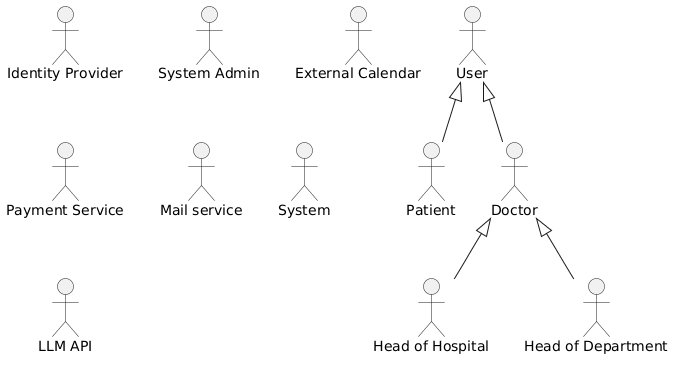
\includegraphics[width=0.8\textwidth]{System_Diagram/Actors.png}
        \captionof{figure}{Actors hierarchy}
    \end{center}
\end{minipage}
\vspace{3em}

\begin{minipage}{\textwidth}
    \subsection{2. Hospital Infrastructure Management}
    This diagram illustrates the interactions for the hospital infrastructure management.
    \begin{center}
        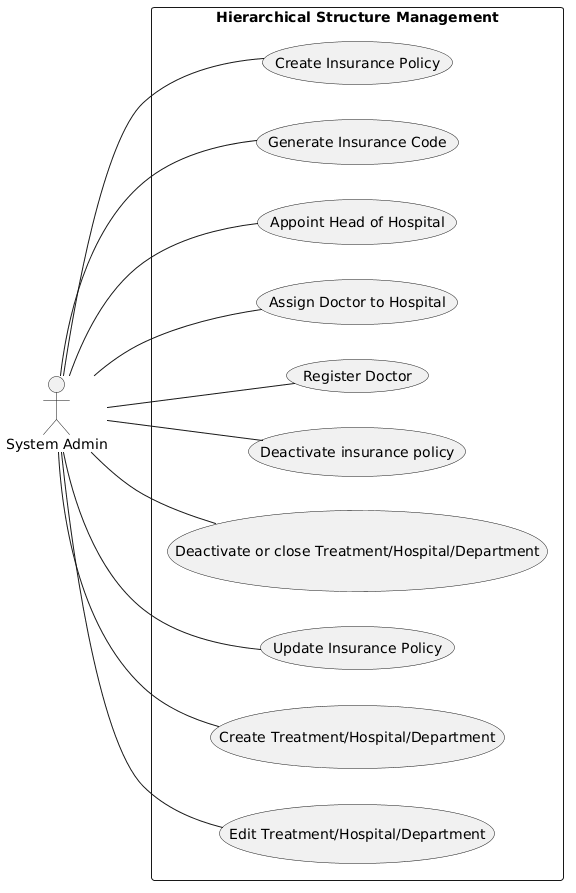
\includegraphics[width=0.8\textwidth]{System_Diagram/HierarchicalManagement.png}
        \captionof{figure}{Hospital infrastructure Management}
    \end{center}
\end{minipage}
\vspace{3em}

\begin{minipage}{\textwidth}
    \subsection{3. Hospital Facility Management}
    This diagram illustrates the interactions for the hospital facility management.
    \begin{center}
        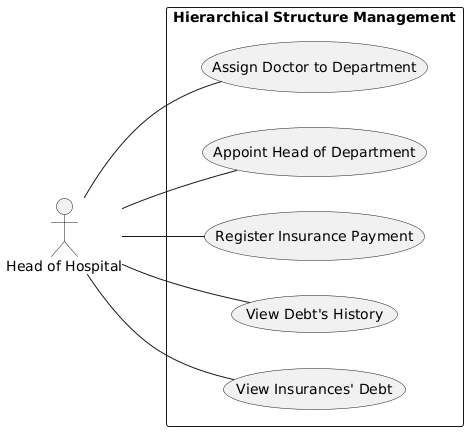
\includegraphics[width=0.8\textwidth]{System_Diagram/HeadOfHospital.png}
        \captionof{figure}{Hospital Facility Management}
    \end{center}
\end{minipage}
\vspace{3em}


\begin{minipage}{\textwidth}
    \subsection{4. Account Management}
    This diagram illustrates the interactions for the hospital structure management.
    \begin{center}
        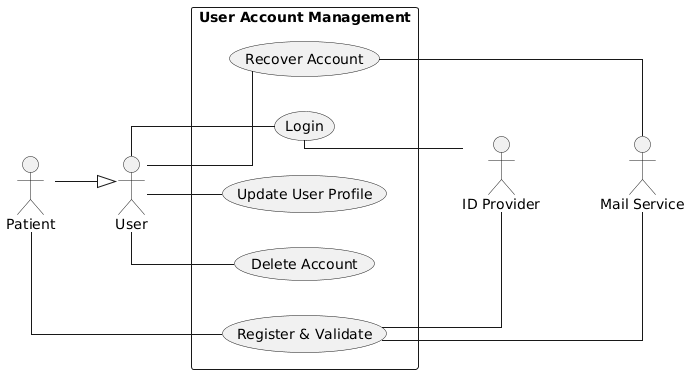
\includegraphics[width=0.8\textwidth]{System_Diagram/AccountManagement.png}
        \captionof{figure}{Account Management}
    \end{center}
\end{minipage}
\vspace{3em}

\begin{minipage}{\textwidth}
    \subsection{5. Appointment and Administration}
    This diagram illustrates the interactions regarding appointments and administration.
    \begin{center}
        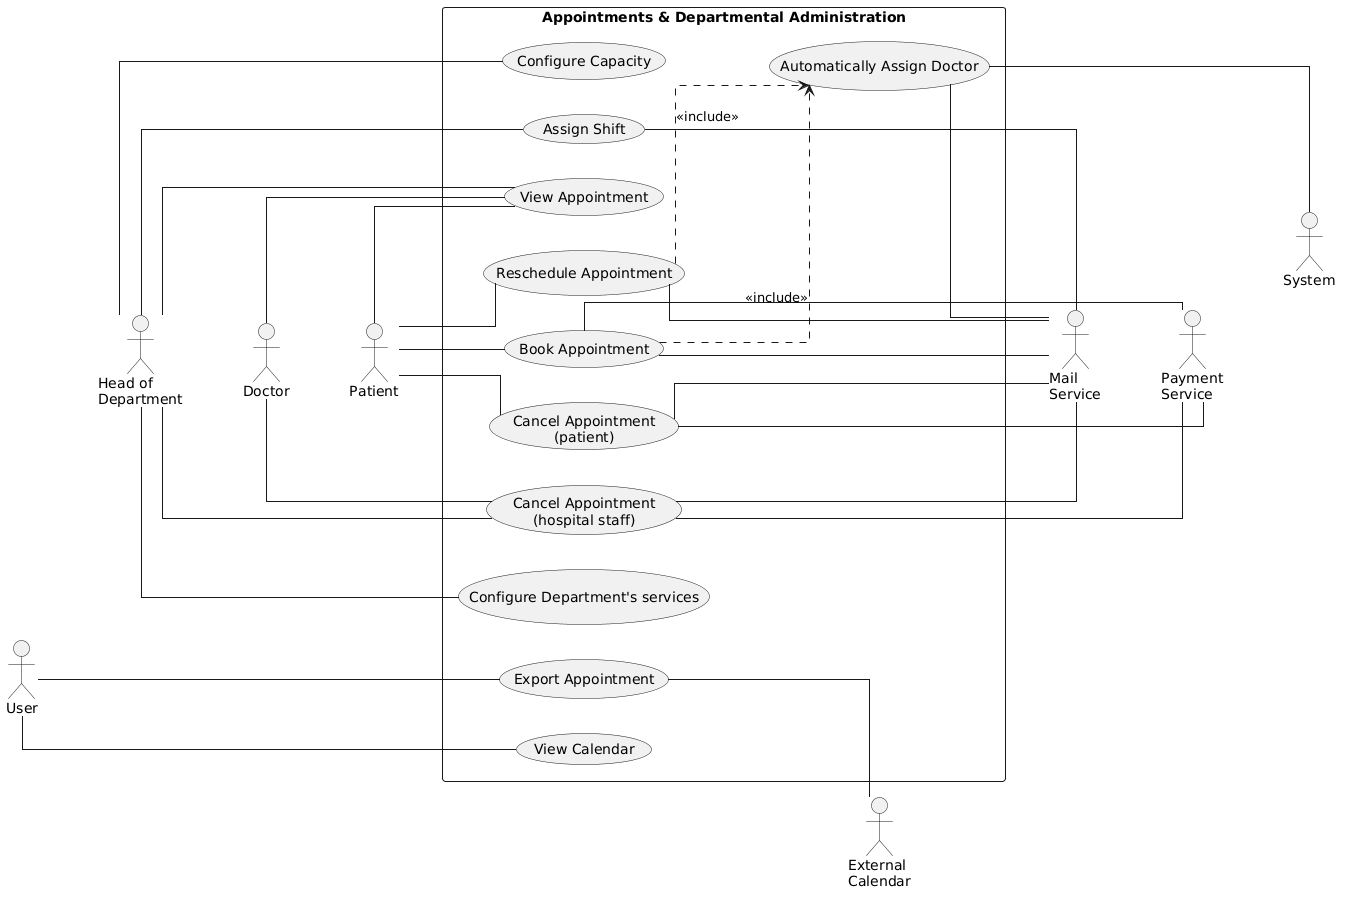
\includegraphics[width=0.8\textwidth]{System_Diagram/AppointmentsAdministration.png}
        \captionof{figure}{Appointment and Administration}
    \end{center}
\end{minipage}
\vspace{3em}

\begin{minipage}{\textwidth}
    \subsection{6. Clinical Operations}
    This diagram illustrates the interactions regarding clinical operations.
    \begin{center}
        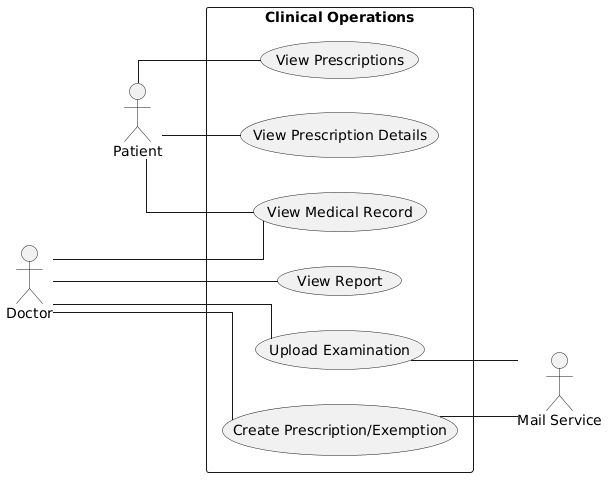
\includegraphics[width=0.8\textwidth]{System_Diagram/ClinicalOp.png}
        \captionof{figure}{Clinical Operations}
    \end{center}
\end{minipage}
\vspace{3em}

\begin{minipage}{\textwidth}
    \subsection{7. Billing }
    This diagram illustrates the interactions regarding payment processing.
    \begin{center}
        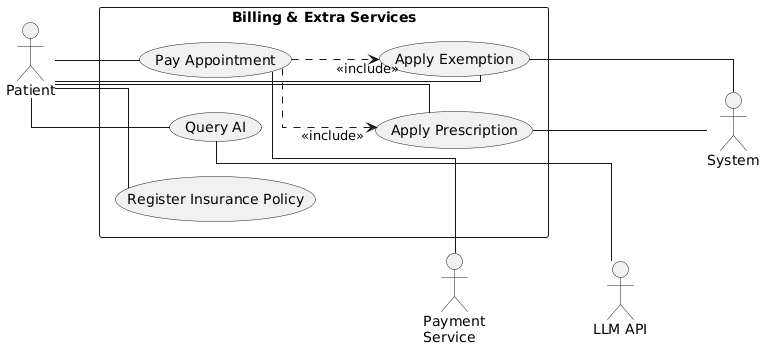
\includegraphics[width=0.8\textwidth]{System_Diagram/Billing.png}
        \captionof{figure}{Billing}
    \end{center}
\end{minipage}
\vspace{3em}



\section{Use Cases}
\phantomsection
\addcontentsline{toc}{subsection}{UC1. Create Treatment / Hospital / Department}
\hypertarget{UC1}{}
\usecaseheader
  {UC1}  % 1: ID
  {Create Treatment / Hospital / Department} % 2: Titolo
  {To allow the System Admin to create basic entities for hospital structures.} % 3: Goal
  {Scope: Hospital structures handling. Level: Primary.} % 4: Scope
  {The user is logged in as a System Admin.} % 5: Preconditions
  {A new Treatment / Hospital / Department is created.} % 6: Success
  {The System remains unchanged. The System returns an error.} % 7: Failed
  {Primary: System Admin. Secondary: Database.} % 8: Actors
  {The System Admin asks the System to create a new Treatment / Hospital / Department.} % 9: Trigger
\begin{ucrequirements}
    FR0.1 & Treatment creation \\ \hline
    FR1.1 & Hospital creation \\ \hline
    FR1.4 & Department creation \\ \hline
    NFR4 & Scalability and capacity \\ \hline   
\end{ucrequirements}
\begin{ucflow}
    1 & The System Admin asks the System to create a new Treatment / Hospital / Department. \\ \hline
    2 & The System Admin fills in the required fields. \\ \hline
    3 & The System Admin saves. \\ \hline
    4 & The System checks if the "name" field is not duplicate. \\ \hline
    5 & The System creates the new Treatment / Hospital / Department in the Database. \\ \hline
    6 & The System returns a success message. \\ \hline
\end{ucflow}

\begin{ucextensions}
    3a & \textbf{The System Admin cancels:}\newline 
         1. The System aborts the creation process.\newline 
         2. Use case ends. \\ \hline
    4a & \textbf{Validity check fails:}\newline 
         1. The System identifies a duplicated name.\newline 
         2. The System returns an error.\newline 
         3. Go to main flow step 2 to perform a correction. \\ \hline
\end{ucextensions}


\phantomsection
\addcontentsline{toc}{subsection}{UC2. Create Insurance Policy}
\hypertarget{UC2}{}
\usecaseheader
  {UC2}  % 1: ID
  {Create Insurance Policy} % 2: Titolo
  {To enable the System Administrator to create new insurance policies shared across all facilities in the healthcare
network.} % 3: Goal
  {Scope: Global Insurance Policy handling. Level: Primary.} % 4: Scope
  {The user is logged in as a System Admin.} % 5: Preconditions
  {A new Insurance Policy is created.} % 6: Success
  {The System remains unchanged. The System returns an error.} % 7: Failed
  {Primary: System Admin. Secondary: Database.} % 8: Actors
  {The System Admin asks the System to create a new Insurance Policy.} % 9: Trigger
\begin{ucrequirements}
    FR9.1 & Create insurance policy \\ \hline
    NFR4 & Scalability and capacity \\ \hline     
\end{ucrequirements}
\begin{ucflow}
    1 & The System Admin asks the System to create a new Insurance Policy. \\ \hline
    2 & The System Admin fills in the required fields. \\ \hline
    3 & The System Admin saves. \\ \hline
    4 & The System checks if the discount percentage is a valid amount. \\ \hline
    5 & The System creates the new Insurance Policy in the Database. \\ \hline
    6 & The System returns a success message. \\ \hline
\end{ucflow}

\begin{ucextensions}
    3a & \textbf{The System Admin cancels:}\newline 
         1. The System aborts the creation process.\newline 
         2. Use case ends. \\ \hline
    4a & \textbf{Validity check fails:}\newline 
         1. The System identifies an invalid amount for the discount percentage.\newline 
         2. The System returns an error.\newline 
         3. Go to main flow step 2 to perform a correction. \\ \hline
\end{ucextensions}


\phantomsection
\addcontentsline{toc}{subsection}{UC3. Create Prescription / Exemption}
\hypertarget{UC3}{}
\usecaseheader
  {UC3}  % 1: ID
  {Create Prescription / Exemption} % 2: Titolo
  {To enable a Doctor to create a new Prescription / Exemption for a specific Patient.} % 3: Goal
  {Scope: Prescriptions / Exemptions. Level: Primary.} % 4: Scope
  {The Doctor is logged into the System.} % 5: Preconditions
  {A new Prescription / Exemption is created and linked to the Patient's profile.} % 6: Success
  {The System remains unchanged. The System returns an error.} % 7: Failed
  {Primary: Doctor. Secondary: Patient, Database, Mail Service.} % 8: Actors
  {The Doctor asks the System to create a new Prescription / Exemption.} % 9: Trigger
\begin{ucrequirements}
    FR29 & Prescription creation \\ \hline
    FR30 & Exemption creation \\ \hline
    NFR4 & Scalability and capacity \\ \hline     
\end{ucrequirements}
\begin{ucflow}
    1 & The Doctor asks the System to create a new Prescription / Exemption. \\ \hline
    2 & The Doctor fills in the required fields, including the selection of the Patient to whom the Prescription / Exemption applies. \\ \hline
    3 & The Doctor saves. \\ \hline
    4 & The System verifies that the selected Patient is valid. \\ \hline    
    5 & The System creates the new Prescription / Exemption in the Database. \\ \hline
    6 & The System returns a success message. \\ \hline
    7 & The Patient is notified via email that the Prescription / Exemption has been linked to their account. \\ \hline
\end{ucflow}

\begin{ucextensions}
    3a & \textbf{The Doctor cancels:}\newline 
         1. The System aborts the creation process.\newline 
         2. Use case ends. \\ \hline
    4a & \textbf{Validity check fails:}\newline 
         1. The System identifies an invalid value for the Patient field.\newline 
         2. The System returns an error.\newline 
         3. Go to main flow step 2 to perform a correction. \\ \hline
\end{ucextensions}


\phantomsection
\addcontentsline{toc}{subsection}{UC4. Upload examination}
\hypertarget{UC4}{}
\usecaseheader
  {UC4}  % 1: ID
  {Upload examination } % 2: Titolo
  {To allow a Doctor to upload and register a completed medical examination, including diagnosis, documents, and notes.} % 3: Goal
  {Scope: Clinical Records Management. Level: Primary.} % 4: Scope
  {A medical examination has been performed and the Doctor is logged into the System..} % 5: Preconditions
  {The examination is successfully uploaded and becomes visible in the Patient’s dashboard.} % 6: Success
  {The System remains unchanged. The System returns an error.} % 7: Failed
  {Primary: Doctor. Secondary: Patient, Database, Mail Service.} % 8: Actors
  {The Doctor asks the System to upload an examination to the Patient clinical record.} % 9: Trigger
\begin{ucrequirements}
    FR33 & Examination upload to Patient clinical record \\ \hline
    NFR4 & Scalability and capacity \\ \hline     
\end{ucrequirements}
\begin{ucflow}
    1 & The Doctor asks the System to upload an examination to the Patient clinical record. \\ \hline
    2 & The Doctor fills in the required fields, including the selection of the Patient to whom the Examination applies. \\ \hline
    3 & The Doctor appends as many attachments as desired \\ \hline
    4 & The Doctor saves. \\ \hline
    5 & The System perform field validations. \\ \hline    
    6 & The System saves the examination record in the Patient clinical record. \\ \hline
    7 & The System returns a success message. \\ \hline
    8 & The Patient is notified via email that a new examination has been uploaded to their record \\ \hline
\end{ucflow}

\begin{ucextensions}
    3a & \textbf{The Doctor cancels:}\newline 
         1. The System aborts the creation process.\newline 
         2. Use case ends. \\ \hline
    5a & \textbf{Validity check fails:}\newline 
         1. The System identifies an invalid value for the Patient field.\newline 
         2. The System returns an error.\newline 
         3. Go to main flow step 2 to perform a correction. \\ \hline
    5b & \textbf{Invalid attachment type:}\newline 
         1. The System identifies an invalid attachment type.\newline 
         2. The System returns an error.\newline 
         3. Go to main flow step 3 to perform a correction. \\ \hline
        
\end{ucextensions}

\phantomsection
\addcontentsline{toc}{subsection}{UC5. Edit Treatment / Hospital / Department}
\hypertarget{UC5}{}
\usecaseheader
  {UC5}  % 1: ID
  {Edit Treatment / Hospital / Department} % 2: Titolo
  {To allow the System Admin to edit basic entities for hospital structure.} % 3: Goal
  {Scope: Hospital structures handling. Level: Primary.} % 4: Scope
  {The user is logged in as a System Admin.} % 5: Preconditions
  {An existing Treatment / Hospital / Department is edited.} % 6: Success
  {The System remains unchanged. The System returns an error.} % 7: Failed
  {Primary: System Admin. Secondary: Database.} % 8: Actors
  {The System Admin asks the System to create a new Treatment / Hospital / Department.} % 9: Trigger
\begin{ucrequirements}
    FR0.2 & Treatment editing \\ \hline
    FR1.2 & Hospital editing \\ \hline
    FR1.5 & Department editing \\ \hline
\end{ucrequirements}
\begin{ucflow}
    1 & The System Admin asks the System to edit an existing Treatment / Hospital / Department. \\ \hline
    2 & The System Admin fills in the required fields. \\ \hline
    3 & The System Admin saves. \\ \hline
    4 & The System checks if the "name" field is not duplicate. \\ \hline
    5 & The System edits the Treatment / Hospital / Department in the Database. \\ \hline
    6 & The System returns a success message. \\ \hline
\end{ucflow}

\begin{ucextensions}
    3a & \textbf{The System Admin cancels:}\newline 
         1. The System aborts the editing process.\newline 
         2. Use case ends. \\ \hline
    4a & \textbf{Validity check fails:}\newline 
         1. The System identifies a duplicated name.\newline 
         2. The System returns an error.\newline 
         3. Go to main flow step 2 to perform a correction. \\ \hline
\end{ucextensions}


\phantomsection
\addcontentsline{toc}{subsection}{UC6. Update Insurance Policy}
\hypertarget{UC6}{}
\usecaseheader
  {UC6}  % 1: ID
  {Update Insurance Policy} % 2: Titolo
  {To enable the System Administrator to edit an existing insurance policies shared across all facilities in the healthcare
network.} % 3: Goal
  {Scope: Global Insurance Policy handling. Level: Primary.} % 4: Scope
  {The user is logged in as a System Admin.} % 5: Preconditions
  {An existing Insurance Policy is edited.} % 6: Success
  {The System remains unchanged. The System returns an error.} % 7: Failed
  {Primary: System Admin. Secondary: Database.} % 8: Actors
  {The System Admin asks the System to edit an existing Insurance Policy.} % 9: Trigger
\begin{ucrequirements}
        FR9.3 & Update insurance policy \\ \hline 
\end{ucrequirements}
\begin{ucflow}
    1 & The System Admin asks the System to update an existing Insurance Policy. \\ \hline
    2 & The System Admin fills in the required fields. \\ \hline
    3 & The System Admin saves. \\ \hline
    4 & The System checks if the discount percentage is a valid amount. \\ \hline
    5 & The System updates the Insurance Policy in the Database. \\ \hline
    6 & The System returns a success message. \\ \hline
\end{ucflow}

\begin{ucextensions}
    3a & \textbf{The System Admin cancels:}\newline 
         1. The System aborts the editing process.\newline 
         2. Use case ends. \\ \hline
    4a & \textbf{Validity check fails:}\newline 
         1. The System identifies an invalid amount for the discount percentage.\newline 
         2. The System returns an error.\newline 
         3. Go to main flow step 2 to perform a correction. \\ \hline
\end{ucextensions}

\phantomsection
\addcontentsline{toc}{subsection}{UC7. Update User Profile}
\hypertarget{UC7}{}
\usecaseheader
  {UC7}  % 1: ID
  {Update User Profile} % 2: Titolo
  {To provide a Registered user with the ability to modify their account information.} % 3: Goal
  {Scope: users account management. Level: Primary.} % 4: Scope
  {The user is logged in.} % 5: Preconditions
  {The account information is successfully updated in the system.} % 6: Success
  {The System remains unchanged. The System returns an error.} % 7: Failed
  {Primary: User. Secondary: Database.} % 8: Actors
  {The authenticated user wants to update their account.} % 9: Trigger
\begin{ucrequirements}
    FR13.2 & Update user profile \\ \hline
\end{ucrequirements}
\begin{ucflow}
    1 & The authenticated user wants to update their account. \\ \hline
    2 & The user edits some fields. \\ \hline
    3 & The user saves. \\ \hline
    4 & The System returns a success message. \\ \hline
\end{ucflow}

\begin{ucextensions}
    3a & \textbf{The user cancels:}\newline 
         1. The System aborts the editing process.\newline 
         2. Use case ends. \\ \hline
\end{ucextensions}


\phantomsection
\addcontentsline{toc}{subsection}{UC8. Deactivate or close Treatment / Hospital / Department}
\hypertarget{UC8}{}
\usecaseheader
  {UC8}  % 1: ID
  {Deactivate or close Treatment / Hospital / Department} % 2: Titolo
  {To allow the System Admin to deactivate or close basic entities for hospital structure.} % 3: Goal
  {Scope: Hospital structures handling. Level: Primary.} % 4: Scope
  {The user is logged in as a System Admin.} % 5: Preconditions
  {An existing Treatment / Hospital / Department is deactivated or closed.} % 6: Success
  {The System remains unchanged. The System returns an error.} % 7: Failed
  {Primary: System Admin. Secondary: Database.} % 8: Actors
  {The System Admin asks the System to deactivate or close a new Treatment / Hospital / Department.} % 9: Trigger
\begin{ucrequirements}
    FR0.3 & Treatment deactivation \\ \hline
    FR1.3 & Hospital closure \\ \hline
    FR1.6 & Department closure \\ \hline
\end{ucrequirements}
\begin{ucflow}
    1 & The System Admin asks the System to deactivate or close an existing Treatment / Hospital / Department. \\ \hline
    2 & The System asks for confirmation. \\ \hline
    3 & The System Admin confirms. \\ \hline
    4 & The System marks the Treatment / Hospital / Department as deactivated or closed. \\ \hline
    5 & The System records date and time of deactivation / closure. \\ \hline
    6 & The System returns a success message. \\ \hline
\end{ucflow}

\begin{ucextensions}
    3a & \textbf{The System Admin cancels:}\newline 
         1. The System aborts the deactivation / closing process.\newline 
         2. Use case ends. \\ \hline
\end{ucextensions}


\phantomsection
\addcontentsline{toc}{subsection}{UC9. Deactivate Insurance Policy}
\hypertarget{UC9}{}
\usecaseheader
  {UC9}  % 1: ID
  {Deactivate Insurance Policy} % 2: Titolo
  {To enable the System Administrator to deactivate an existing insurance policies shared across all facilities in the healthcare
network.} % 3: Goal
  {Scope: Global Insurance Policy handling. Level: Primary.} % 4: Scope
  {The user is logged in as a System Admin.} % 5: Preconditions
  {An existing Insurance Policy is deactivated.} % 6: Success
  {The System remains unchanged. The System returns an error.} % 7: Failed
  {Primary: System Admin. Secondary: Database.} % 8: Actors
  {The System Admin asks the System to deactivate an existing Insurance Policy.} % 9: Trigger
\begin{ucrequirements}
    FR9.4 & Delete insurance policy \\ \hline
\end{ucrequirements}
\begin{ucflow}
    1 & The System Admin asks the System to deactivate an existing Insurance Policy. \\ \hline
    2 & The System asks for confirmation. \\ \hline
    3 & The System Admin confirms. \\ \hline
    4 & The System marks the Insurance Policy as deactivated. \\ \hline
    5 & The System records date and time of deactivation. \\ \hline
    6 & The System returns a success message. \\ \hline
\end{ucflow}

\begin{ucextensions}
    3a & \textbf{The System Admin cancels:}\newline 
         1. The System aborts the editing process.\newline 
         2. Use case ends. \\ \hline
\end{ucextensions}

\phantomsection
\addcontentsline{toc}{subsection}{UC10. Cancel appointment (Patient)}
\hypertarget{UC10}{}
\usecaseheader
  {UC10}  % 1: ID
  {Cancel appointment (Patient)} % 2: Titolo
  {To enable Patient to cancel a booked medical appointment} % 3: Goal
  {Scope: Appointment management. Level: Primary.} % 4: Scope
  {The Patient is logged in.} % 5: Preconditions
  {An existing medical appointment is deleted.} % 6: Success
  {The System remains unchanged. The System returns an error.} % 7: Failed
  {Primary: Patient. Secondary: Database, Payment Service, Mail Service.} % 8: Actors
  {Patient asks the System to cancel a booked appointment.} % 9: Trigger
\begin{ucrequirements}
    FR16.2 & Cancel appointment (Patient) \\ \hline
    \end{ucrequirements}
\begin{ucflow}
    1 & Patient asks the System to cancel a booked appointment. \\ \hline
    2 & The System asks for confirmation. \\ \hline
    3 & The Patient confirms. \\ \hline
    4 & The System performs validity check. \\ \hline
    5 & The System cancels the appointment. \\ \hline
    6 & The Patient is refunded. \\ \hline
    7 & The System returns a success message. \\ \hline
\end{ucflow}

\begin{ucextensions}
    3a & \textbf{The Patient cancels:}\newline 
         1. The System aborts the editing process.\newline 
         2. Use case ends. \\ \hline
    4a & \textbf{Late canceling:}\newline 
         1. The System identifies that the appointment is in less than 48 hours.\newline 
         2. Cancellation is aborted.\newline 
         3. The System returns an error.\newline 
         4. Use case ends. \\ \hline
    6a & \textbf{Appointment not paid:}\newline 
         1. The System checks if the appointment was paid ahead.\newline 
         2. If not, proceed to step 7 (refund is skipped).\\ \hline
\end{ucextensions}

\phantomsection
\addcontentsline{toc}{subsection}{UC11. Cancel appointment (hospital staff)}
\hypertarget{UC11}{}
\usecaseheader
  {UC11}  % 1: ID
  {Cancel appointment (Hospital staff)} % 2: Titolo
  {To enable Doctor / Head of Department to cancel a booked medical appointment} % 3: Goal
  {Scope: Appointment management. Level: Primary.} % 4: Scope
  {The Doctor / Head of Department is logged in.} % 5: Preconditions
  {An existing medical appointment is deleted.} % 6: Success
  {The System remains unchanged. The System returns an error.} % 7: Failed
  {Primary: Doctor / Head of Department. Secondary: Database, Payment Service, Mail Service.} % 8: Actors
  {The Doctor / Head of Department asks the System to cancel a booked appointment.} % 9: Trigger
\begin{ucrequirements}
    FR35.2 & Cancel appointment (Doctor)\\ \hline
    FR36.2 & Cancel appointment (Head of Department) \\ \hline\end{ucrequirements}
\begin{ucflow}
    1 & The Doctor / Head of Department asks the System to cancel a booked appointment. \\ \hline
    2 & The Doctor / Head of Department provides a cancellation reason. \\ \hline
    3 & The Doctor / Head of Department confirms. \\ \hline
    4 & The System performs validity check. \\ \hline
    5 & The System cancels the appointment. \\ \hline
    6 & The Patient is notified via email about the appointment cancellation with the reason. \\ \hline
    7 & The Patient is refunded. \\ \hline
    8 & The System returns a success message. \\ \hline
\end{ucflow}

\begin{ucextensions}
    3a & \textbf{The Doctor / Head of Department cancels:}\newline 
         1. The System aborts the editing process.\newline 
         2. Use case ends. \\ \hline
    7a & \textbf{Appointment not paid:}\newline 
         1. The System checks if the appointment was paid ahead.\newline 
         2. If not, proceed to step 7 (refund is skipped).\\ \hline
\end{ucextensions}

\phantomsection
\addcontentsline{toc}{subsection}{UC12. Register Doctor}
\hypertarget{UC12}{}
\usecaseheader
  {UC12} % 1: ID
  {Register Doctor} % 2: Titolo
  {A System Admin wants to add a new Doctor to the hospital’s digital infrastructure.} % 3: Goal
  {Scope: Hospital structures handling. Level: Primary.} % 4: Scope
  {The user is logged in as a System Admin. The relevant hospital structure already exists.} % 5: Preconditions
  {The Doctor is successfully saved in the Database, and a set of one-time credentials is provided to the System Admin.} % 6: Success
  {The registration is aborted due to invalid data or duplication; no credentials are created.} % 7: Failed
  {Primary: System Admin. Secondary: Database.} % 8: Actors
  {The System Admin asks the System to create a new Doctor account.} % 9: Trigger
\begin{ucrequirements}
    FR1.7 & Doctor registration \\ \hline
\end{ucrequirements}
\begin{ucflow}
    1 & The System Admin asks the System to create a new Doctor account. \\ \hline
    2 & The System Admin fills in the required fields, including Doctor's personal data. \\ \hline
    3 & The System Admin saves. \\ \hline
    4 & The System checks if the "name" field is not duplicate. \\ \hline
    5 & The System creates the new Doctor account in the Database. \\ \hline
    6 & The System returns the new account credentials, which are displayed just once. \\ \hline
\end{ucflow}

\begin{ucextensions}
    3a & \textbf{The System Admin cancels:}\newline 
         1. The System aborts the creation process.\newline 
         2. Use case ends. \\ \hline
    4a & \textbf{Validity check fails:}\newline 
         1. The System identifies duplicated personal data for the Doctor.\newline 
         2. The System returns an error.\newline 
         3. Go to main flow step 2 to perform a correction. \\ \hline
\end{ucextensions}


\phantomsection
\addcontentsline{toc}{subsection}{UC13. Assign Doctor}
\hypertarget{UC13}{}
\usecaseheader
  {UC13} % 1: ID
  {Assign Doctor} % 2: Titolo
  {To enable the System Administrator to assign a Registered Doctor to operate within a specific hospital structure.} % 3: Goal
  {Scope: Hospital structures handling. Level: Primary.} % 4: Scope
  {The user is logged as a System Admin. The specific hospital has been created. The Doctor is registered in the System.} % 5: Preconditions
  {The selected Doctor is successfully assigned to the specified hospital.} % 6: Success
  {Doctor assignment fails. The previous assignment remains unchanged.} % 7: Failed
  {Primary: System Admin. Secondary: Database.} % 8: Actors
  {System Admin wants to assign a Doctor to a specific hospital structure.} % 9: Trigger
\begin{ucrequirements}
    FR1.8 & Doctor assignment \\ \hline
\end{ucrequirements}
\begin{ucflow}
    1 & System Admin wants to assign a Doctor to a specific hospital structure. \\ \hline
    2 & System Admin picks the selected Doctor from the set of registered Doctors. \\ \hline
    3 & System Admin saves. \\ \hline
    4 & The System asks for confirmation. \\ \hline
    5 & System Admin confirms. \\ \hline
    6 & The System performs validity checks. \\ \hline
    7 & The Doctor is assigned to the hospital and the System status is updated. \\ \hline
\end{ucflow}

\begin{ucextensions}
    5a & \textbf{Cancel operation:}\newline 
         1. System Admin cancels.\newline 
         2. No changes are made to the System.\newline 
         3. Use case ends. \\ \hline
    6a & \textbf{Doctor already assigned:}\newline 
         1. The System finds the specified Doctor already assigned.\newline 
         2. The System asks for permission to reassign already assigned Doctor.\newline 
         3. The System Administrator confirms. (If not, the use case ends) \newline
         4. Go to main flow step 6. \\ \hline
\end{ucextensions}

\phantomsection
\addcontentsline{toc}{subsection}{UC14. Appoint Head of Hospital}
\hypertarget{UC14}{}
\usecaseheader
  {UC14} % 1: ID
  {Appoint Head of Hospital} % 2: Titolo
  {To enable the System Administrator to appoint a Registered Doctor to the strategic role of Head of Hospital for a specific facility.} % 3: Goal
  {Scope: Hospital structures handling. Level: Primary.} % 4: Scope
  {The user is logged in as a System Administrator. The specific hospital has been created. The Doctor is already registered in the System.} % 5: Preconditions
  {The selected Doctor is successfully appointed as Head of Hospital.} % 6: Success
  {The appointment fails; the System state remains unchanged and the previous head (if any) remains in place.} % 7: Failed
  {Primary: System Administrator. 
Secondary: Database.} % 8: Actors
  {The System Administrator wants to appoint a Doctor as Head of Hospital.} % 9: Trigger
\begin{ucrequirements}
    FR5 & Strategic role appointment (Head of Hospital) \\ \hline
\end{ucrequirements}
\begin{ucflow}
    1 & The System Administrator wants to appoint a Doctor as Head of Hospital. \\ \hline
    2 & The Admin selects the desired Doctor from the list of Registered Doctors. \\ \hline
    3 & The Admin saves. \\ \hline
    4 & The System prompts the Admin with a confirmation message. \\ \hline
    5 & The Admin confirms. \\ \hline
    6 & The System performs validity checks. \\ \hline
    7 & The Doctor is appointed as Head of Hospital and the System status is updated. \\ \hline
\end{ucflow}

\begin{ucextensions}
    2a & \textbf{Already existing Head of Hospital:}\newline 
         1. The System prompts that there is another Head of Hospital for that structure. \newline 
         2. The System asks if the admin wants to change the Head of Hospital. \newline 
         3. Admin confirms. \newline 
         4. Resume at Main Flow Step 6. \\ \hline
    5a & \textbf{Operation canceled:}\newline 
         1. Admin cancels the operation. \newline 
         2. No changes are made to the Database. \newline 
         3. Use case ends. \\ \hline
    6a & \textbf{Doctor not found:}\newline 
         1. System cannot find the selected Doctor. \newline 
         2. Operation is aborted. \newline 
         3. System returns an error. \newline 
         4. Use case ends. \\ \hline
\end{ucextensions}

\phantomsection
\addcontentsline{toc}{subsection}{UC15. Appoint Head of Department}
\hypertarget{UC15}{}
\usecaseheader
  {UC15} % 1: ID
  {Appoint Head of Department} % 2: Titolo
  {To enable the Head of Hospital to appoint a Registered Doctor to the tactical role of Head of Department within their facility.} % 3: Goal
  {Scope: Hospital structures handling. Level: Primary.} % 4: Scope
  {The user is logged as a Head of Hospital. The specific department has been created. The Doctor is registered in the System.} % 5: Preconditions
  {The selected Doctor is successfully appointed as Head of Department.} % 6: Success
  {Head of Department appointment fails. The System remains unchanged.} % 7: Failed
  {Primary: Head of Hospital. 
Secondary: Database.} % 8: Actors
  {The Head of Hospital wants to appoint a Doctor as Head of Department.} % 9: Trigger
\begin{ucrequirements}
    FR3 & Tactical role appointment (Head of Department) \\ \hline
\end{ucrequirements}
\begin{ucflow}
    1 & The Head of Hospital wants to appoint a Doctor as Head of Department. \\ \hline
    2 & The Head of Hospital picks the selected Doctor from the set of Registered Doctors in their facility. \\ \hline
    3 & The Head of Hospital saves. \\ \hline
    4 & The Head of Hospital is prompted with a confirmation message. \\ \hline
    5 & The Head of Hospital confirms. \\ \hline
    6 & The System performs validity checks. \\ \hline
    7 & The Doctor is appointed as Head of Department and the System status is updated. \\ \hline
\end{ucflow}

\begin{ucextensions}
    2a & \textbf{Already existing Head of Department:}\newline 
         1. The System prompts that there is another Head of Department for that department. \newline 
         2. The System ask if the Head of Hospital wants to change the Head of Department. \newline 
         3. Head of Hospital confirms. \newline 
         4. Resume at Main Flow Step 6. \\ \hline
    5a & \textbf{Operation canceled:}\newline 
         1. Head of Hospital cancels the operation. \newline 
         2. No changes are made to the Database. \newline 
         3. Use case ends. \\ \hline
    6a & \textbf{Doctor not found:}\newline 
         1. System cannot find the selected Doctor. \newline 
         2. Operation is aborted. \newline 
         3. System returns an error. \newline 
         4. Use case ends. \\ \hline
\end{ucextensions}

\phantomsection
\addcontentsline{toc}{subsection}{UC16. Assign Doctor to Department}
\hypertarget{UC16}{}
\usecaseheader
  {UC16} % 1: ID
  {Allocate facility's Doctors} % 2: Titolo
  {To enable the Head of Hospital to allocate operational resources to a specific department within their facility.} % 3: Goal
  {Scope: Hospital structures handling. Level: Primary.} % 4: Scope
  {The user is logged in as a Head of Hospital. The specific departments have been created. The specific Doctors are registered in the System.} % 5: Preconditions
  {The selected Doctors are successfully allocated to the selected department.} % 6: Success
  {The Doctors’ allocation fails; the previous allocation remains unchanged.} % 7: Failed
  {Primary: Head of Hospital. 
Secondary: Database.} % 8: Actors
  {The Head of Hospital wants to allocate Doctors for a specific facility.} % 9: Trigger
\begin{ucrequirements}
    FR4 & Facility Doctors allocation \\ \hline
\end{ucrequirements}
\begin{ucflow}
    1 & The Head of Hospital wants to allocate Doctors for a specific facility. \\ \hline
    2 & The Head of Hospital picks the selected Doctors from the set of Registered Doctors within the System. \\ \hline
    3 & The Head of Hospital saves the selection. \\ \hline
    4 & The System performs validity checks. \\ \hline
    5 & The Doctors are allocated to the department and the System status is updated. \\ \hline
\end{ucflow}

\begin{ucextensions}
    4a & \textbf{Doctors already allocated:}\newline 
         1. The System identifies that the specified Doctors are already allocated to another department. \newline 
         2. The System asks for permission to reassign the already allocated Doctors. \newline 
         3. The Head of Hospital confirms (if not, the use case ends). \newline 
         4. Resume at Main Flow Step 6. \\ \hline
\end{ucextensions}

\phantomsection
\addcontentsline{toc}{subsection}{UC17. Configure Department's services}
\hypertarget{UC17}{}
\usecaseheader
  {UC17} % 1: ID
  {Configure Department's services} % 2: Titolo
  {To enable the Head of Department to configure and update the list of medical treatments offered by their specific department.} % 3: Goal
  {Scope: Managing the global hospital catalog. Level: Primary.} % 4: Scope
  {The hospital and department have been created, and the global catalog has been populated.} % 5: Preconditions
  {The offered treatments for the specific department are successfully updated in the System.} % 6: Success
  {The changes are not saved; the department's treatment offerings remain in their previous state.} % 7: Failed
  {Primary: Head of Department. 
Secondary: Database, Global Treatment Catalog.} % 8: Actors
  {The Head of Department wants to configure the list of medical treatments offered for their department.} % 9: Trigger
\begin{ucrequirements}
    FR5 & Departmental service configuration \\ \hline
\end{ucrequirements}

\begin{ucflow}
    1 & The Head of Department wants to configure the list of medical treatments offered for their department. \\ \hline
    2 & The System displays all available treatments retrieved from the global catalog. \\ \hline
    3 & The Head of Department disables or enables a specific treatment. \\ \hline
    4 & The Head of Department clicks saves. \\ \hline
    5 & The System performs validity checks. \\ \hline
    6 & The System updates the department records and confirms the changes to the user. \\ \hline
\end{ucflow}

\begin{ucextensions}
    5a & \textbf{Data validation fails:}\newline 
         1. The System cannot find selected treatment in the Database. \newline 
         2. Operation is aborted. \newline 
         3. The System prompts an error message. \newline 
         4. Use case ends. \\ \hline
\end{ucextensions}

\phantomsection
\addcontentsline{toc}{subsection}{UC18. View Insurances' Debts}
\hypertarget{UC18}{}
\usecaseheader
  {UC18} % 1: ID
  {View Insurances' Debts} % 2: Titolo
  {To enable the Head of Hospital to view and monitor the outstanding financial debt owed by insurance companies to their facility.} % 3: Goal
  {Scope: Managing insurance. Level: Primary.} % 4: Scope
  {The user is logged in with Head of Hospital privileges.} % 5: Preconditions
  {The Head of Hospital successfully views the current debt breakdown.} % 6: Success
  {The System fails to retrieve financial records; the Head of Hospital is notified of the data unavailability.} % 7: Failed
  {Primary: Head of Hospital. 
Secondary: Database.} % 8: Actors
  {The Head of Hospital wants to monitor the outstanding debt owned by insurance companies to their facility.} % 9: Trigger
\begin{ucrequirements}
    FR6.1 & Insurance debt dashboard \\ \hline
\end{ucrequirements}

\begin{ucflow}
    1 & The Head of Hospital wants to monitor the outstanding debt owned by insurance companies to their facility. \\ \hline
    2 & The System displays a list of debt amounts categorized by each individual insurance company. \\ \hline
    3 & The Head of Hospital reviews the high-level financial summary. \\ \hline
\end{ucflow}

\begin{ucextensions}
    1a & \textbf{Data not found:}\newline 
         1. The System fails to retrieve insurance data. \newline 
         2. The Head of Hospital is prompted with an error message. \newline 
         3. Use case ends. \\ \hline
    2a & \textbf{View historical records:}\newline 
         1. The Head of Hospital wants to monitor historical records. \newline 
         2. The System displays a detailed historical debt record. \\ \hline
\end{ucextensions}


\phantomsection
\addcontentsline{toc}{subsection}{UC19. Insurance Debt History}
\hypertarget{UC19}{}
\usecaseheader
  {UC19}  % 1: ID
  {Insurance Debt History} % 2: Titolo
  {To enable the Head of Hospital to view the detailed information of a specific insurance company’s debt history regarding their facility.} % 3: Goal
  {Scope: Managing insurance. Level: Primary.} % 4: Scope
  {The user is logged in as Head of Hospital, the insurance company has some insurance policy registered in the System.} % 5: Preconditions
  {The System successfully retrieves and displays the debt history for the specific insurance company.} % 6: Success
  {The System is unable to display information and returns an error.} % 7: Failed
  {Primary: Head of Hospital. Secondary: Database.} % 8: Actors
  {The Head of Hospital wants to see the debt history for a specific insurance company.} % 9: Trigger
\begin{ucrequirements}
    FR6.2 & Insurance Debt History \\ \hline
\end{ucrequirements}
\begin{ucflow}
    1 & The Head of Hospital selects a specific insurance company to view its debt history. \\ \hline
    2 & The System validates the user's access rights for this specific action. \\ \hline
    3 & The System queries the Database to retrieve the current outstanding debt. \\ \hline
    4 & The System queries the Database to retrieve previous debt settlements along with their associated dates and amounts. \\ \hline
    5 & The System displays the comprehensive debt history to the Head of Hospital. \\ \hline
\end{ucflow}

\begin{ucextensions}
    2a & \textbf{Access validation fails:}\newline 
         1. The System identifies that the user lacks the specific rights to view this detailed record.\newline 
         2. The System prompts an error.\newline 
         3. The view process is aborted. Use case ends. \\ \hline
    3a & \textbf{Entity not found:}\newline 
         1. The System is unable to locate the insurance company in the Database.\newline 
         2. The System prompts an error message explaining that the entity is no longer available.\newline 
         3. Use case ends. \\ \hline
    4a & \textbf{No previous debt history:}\newline
         1. The System finds no past settlements for the selected insurance company.\newline
         2. The System displays an error. \newline
         3. Use case ends. \\ \hline
         
\end{ucextensions}

\phantomsection
\addcontentsline{toc}{subsection}{UC20. Register insurance payment}
\hypertarget{UC20}{}
\usecaseheader
  {UC20} % 1: ID
  {Register insurance payment} % 2: Titolo
  {To enable the Head of Hospital to manually settle and clear the outstanding financial balance owed by a specific insurance company to their facility.} % 3: Goal
  {Scope: Managing insurance. Level: Primary.} % 4: Scope
  {The user is logged in as the Head of Hospital. The hospital exists, an outstanding debt is present, and the insurance company has paid out the debt.} % 5: Preconditions
  {The outstanding debt is marked as settled, and the transaction is recorded in the System.} % 6: Success
  {The settlement process is cancelled or fails; the debt remains unchanged.} % 7: Failed
  {Primary: Head of Hospital. 
Secondary: Database.} % 8: Actors
  {The Head of Hospital wants to settle the outstanding debt for a specific insurance company.} % 9: Trigger
\begin{ucrequirements}
    FR7 & Manual settlement of insurance debt \\ \hline
\end{ucrequirements}

\begin{ucflow}
    1 & The Head of Hospital wants to settle the outstanding debt for a specific insurance company. \\ \hline
    2 & The Head of Hospital fills in the payment data. \\ \hline
    3 & The Head of Hospital saves. \\ \hline
    4 & The System validates the input fields. \\ \hline
    5 & The System displays a confirmation alert showing the exact amount being settled. \\ \hline
    6 & The Head of Hospital confirms. \\ \hline
    7 & The System updates the Database to reflect the settled status and adjusts the total debt. \\ \hline
    8 & The System provides a success notification. \\ \hline
\end{ucflow}

\begin{ucextensions}
    4a & \textbf{Validity check fails:}\newline 
         1. The System identifies an invalid field for the payment details. \newline 
         2. The System displays an error message . \newline 
         3. Resume at Main Flow Step 2. \\ \hline
    6a & \textbf{Head of Hospital cancels:}\newline 
         1. No changes are made to the Database. \newline 
         2. The settlement process is immediately terminated. \newline 
         3. Use case ends. \\ \hline
\end{ucextensions}

\phantomsection
\addcontentsline{toc}{subsection}{UC21. Departmental capacity configuration}
\hypertarget{UC21}{}
\usecaseheader
  {UC21} % 1: ID
  {Departmental operational management} % 2: Titolo
  {To enable the Head of Department to configure the operational capacity of the department.} % 3: Goal
  {Scope: Hospital structures handling. Level: Primary.} % 4: Scope
  {The user is logged in as a Head of Department.} % 5: Preconditions
  {The operational capacity is successfully updated.} % 6: Success
  {The operational capacity remains unchanged.} % 7: Failed
  {Primary: Head of Department. 
Secondary: Database} % 8: Actors
  {The Head of Department wants to configure operational capacity.} % 9: Trigger
\begin{ucrequirements}
    FR8.1 & Department capacity configuration \\ \hline
\end{ucrequirements}
\begin{ucflow}
        1 & The Head of Department wants to configure operational capacity (number and type of rooms). \\ \hline 
        2 & The Head of Department updates the desired fields and saves. \\ \hline 
        3 & The System validates input fields.\\ \hline 
        4 & The System updates the Database to reflect the new operational capacity. \\ \hline
        5 & The System provides a success notification. \\ \hline
\end{ucflow}

\begin{ucextensions}
    3a & \textbf{Validity check fails:}\newline 
         1. The System identifies an invalid field for the operational capacity. \newline 
         2. The System displays an error message highlighting the invalid field. \newline 
         3. Resume at Main Flow Step 2. \\ \hline
\end{ucextensions}

\phantomsection
\addcontentsline{toc}{subsection}{UC22. Generate Insurance Policy code}
\hypertarget{UC22}{}
\usecaseheader
  {UC22} % 1: ID
  {Generate Insurance Policy code} % 2: Titolo
  {To provide the System Administrator the ability to generate the insurance policy code.} % 3: Goal
  {Scope: Insurance policies management. Level: Primary.} % 4: Scope
  {The insurance policy has been created and the Patient is registered in the System.} % 5: Preconditions
  {The unique code is successfully created.} % 6: Success
  {The unique code is not created.} % 7: Failed
  {Primary: System Admin. 
Secondary: Database.} % 8: Actors
  {The System Administrator wants to generate a unique insurance code for a specific policy.} % 9: Trigger
\begin{ucrequirements}
    FR10 & Simulated Insurance code generation \\ \hline
\end{ucrequirements}

\begin{ucflow}
    1 & The System Administrator wants to generate a unique insurance code for a specific policy. \\ \hline
    2 & The System generate a code. \\ \hline
\end{ucflow}

\begin{ucextensions}
    2a & \textbf{System error during generation:}\newline 
         1. The System encounters a Database or internal error and cannot generate the code. \newline 
         2. The System displays an error message prompting to try again. \newline 
         3. Use case ends. \\ \hline
\end{ucextensions}

\phantomsection
\addcontentsline{toc}{subsection}{UC23. User registration and validation}
\hypertarget{UC23}{}
\usecaseheader
  {UC23} % 1: ID
  {User registration and validation} % 2: Titolo
  {To allow an Unregistered Patient to create and validate an account within the System} % 3: Goal
  {Scope: Users account management. Level: Primary Task.} % 4: Scope
  {The Patient is not authenticated and does not have an active account.} % 5: Preconditions
  {A new account is registered in the System and successfully validated.} % 6: Success
  {No new account is created, or the account remains unverified; the user is prompted with an error message.} % 7: Failed
  {Primary: Patient. Secondary: Database, Mail Service, Identity Provider (SPID/CIE).} % 8: Actors
  {The Unregistered Patient wants to register in the System.} % 9: Trigger
\begin{ucrequirements}
    FR11.1 & User registration \\ \hline
    FR11.2 & User validation \\ \hline
    NFR0 & Security and privacy \\ \hline
    NFR6 & SPID/CIE-based registration and authentication \\ \hline
    NFR7 & Login validity period \\ \hline
\end{ucrequirements}

\begin{ucflow}
    1 & The System asks the Unregistered Patient to insert their email and personal information. \\ \hline
    2 & The Patient fills in the required information. \\ \hline
    3 & The Unregistered Patient submits. \\ \hline
    4 & The System validates the input fields. \\ \hline
    5 & The Patient is prompted to create a password. \\ \hline
    6 & The Patient submits a password. \\ \hline
    7 & The System checks password security (complexity and strength). \\ \hline
    8 & The System creates a new unverified account in the Database. \\ \hline
    9 & The System sends a verification token to the provided email address via the Mail Service. \\ \hline
    10 & The User accesses their mailbox and clicks on the validation link. \\ \hline
    11 & The System retrieves the validation token sent with the request. \\ \hline
    12 & The System checks for token validity and matching records in the Database. \\ \hline
    13 & The System marks the account as verified and active. \\ \hline
    14 & The System automatically logs the user in and redirects them to the home page. \\ \hline
\end{ucflow}

\begin{ucextensions}
    4a & \textbf{Duplicated fiscal code:}\newline 
         1. The System identifies a duplicated fiscal code. \newline 
         2. The Patient is prompted with an error message highlighting the invalid field. \newline 
         3. Resume at Main Flow Step 2. \\ \hline
    4b & \textbf{Email already taken:}\newline 
         1. The System finds another account already associated with the provided email. \newline 
         2. The Patient is prompted with an error message suggesting to log in or reset the password. \newline 
         3. Use case ends. \\ \hline
    6a & \textbf{Password security check fails:}\newline 
         1. The System identifies the provided password as unsafe or too simple. \newline 
         2. The System prompts an error message with security requirements. \newline 
         3. Resume at Main Flow Step 5. \\ \hline
    11a & \textbf{Invalid or Expired validation token:}\newline 
         1. The System identifies that the token from the email link is invalid or has expired.\newline 
         2. The Patient is prompted with an error message and asked if they want to receive a new validation email.\newline 
         3. The Patient either confirms (go to Main flow step 9) or declines (use case ends). \\ \hline
\end{ucextensions}

\begin{ucsubvariations}
    2a & \textbf{SPID or CIE register:}\newline 
         1. The User selects to register using a National Digital Identity Provider (SPID/CIE).\newline 
         2. Authentication is performed by the external authority, which returns a secure token.\newline 
         3. The System maps the token to the corresponding user account.\newline
         4. Use case ends. \\ \hline
\end{ucsubvariations}

\phantomsection
\addcontentsline{toc}{subsection}{UC24. User Login}
\hypertarget{UC24}{}
\usecaseheader
  {UC24} % 1: ID
  {User Login} % 2: Titolo
  {To allow a registered user to securely log into their account.} % 3: Goal
  {Scope: Account management. Level: Primary Task.} % 4: Scope
  {The user has a registered and validated account in the System.} % 5: Preconditions
  {The user successfully logs in and is redirected to their dashboard.} % 6: Success
  {The login fails, and the user is prompted with an error message.} % 7: Failed
  {Primary: User. Secondary: Database, Identity Provider (SPID/CIE).} % 8: Actors
  {The user wants to log into the System.} % 9: Trigger
\begin{ucrequirements}
    FR11.3 & User login \\ \hline
    NFR0 & Security and privacy \\ \hline
    NFR6 & SPID/CIE-based registration and authentication \\ \hline
    NFR7 & Login validity period \\ \hline
\end{ucrequirements}

\begin{ucflow}
    1 & The User inputs their registered email and password. \\ \hline
    2 & The System verifies the provided credentials against the Database. \\ \hline
    3 & The user successfully logs in. \\ \hline
\end{ucflow}

\begin{ucextensions}
    2a & \textbf{Invalid Credentials:}\newline 
         1. The System identifies that the provided email or password is incorrect. \newline 
         2. The System displays an error message. \newline
         3. Resume at Main Flow Step 1. \\ \hline
    3a & \textbf{Mandatory Password Change:}\newline 
         1. The System detects that the User (e.g., a newly registered Doctor) is logging in for the first time using a System-generated default password. \newline 
         2. The User is prompted to update their credentials through the \hyperlink{UC26}{Account recovery} use case. \newline
         3. Use case ends. \\ \hline
\end{ucextensions}


\begin{ucsubvariations}
    1a & \textbf{SPID or CIE login:}\newline 
         1. The User selects to log in using a National Digital Identity Provider (SPID/CIE).\newline 
         2. Authentication is performed by the external authority, which returns a secure token.\newline 
         3. The System maps the token to the corresponding user account.\newline
         4. Resume at Main Flow Step 3. \\ \hline
\end{ucsubvariations}

\phantomsection
\addcontentsline{toc}{subsection}{UC25. Automated Doctor Assignment}
\hypertarget{UC25}{}
\usecaseheader
  {UC25} % 1: ID
  {Automated Doctor Assignment} % 2: Titolo
  {To automatically assign the most suitable Doctor to a newly requested appointment based on specialty and continuity of care.} % 3: Goal
  {Scope: Doctor assignment. Level: Subfunction.} % 4: Scope
  {The calling use case has provided the examination type, requested date, hospital, and available room.} % 5: Preconditions
  {A suitable Doctor is successfully assigned to the appointment.} % 6: Success
  {No Doctor is assigned; the System notifies the Head of Department of the failure.} % 7: Failed
  {Primary: System. 
Secondary: Patient, Database, Mail Service, Head of Department.} % 8: Actors
  {The use case is triggered automatically when a Patient is booking or rescheduling an appointment.} % 9: Trigger
\begin{ucrequirements}
    FR12 & Automated Doctor assignment\\ \hline
    NFR1 & Algorithm performance\\ \hline
\end{ucrequirements}

\begin{ucflow}
    1 & The use case is triggered automatically when a Patient is booking or rescheduling an appointment \\ \hline
    2 & The System filters for Doctors whose specialty matches the requested examination type. \\ \hline
    3 & The System filters for Doctors that have already visited the Patient. \\ \hline
    4 & The System picks the Doctor with the earliest availability closest to the requested date, provided they are available within a 30-day window. \\ \hline
\end{ucflow}

\begin{ucextensions}
    2a & \textbf{No Doctor found with required specialty:}\newline 
         1. The System sends a notification to the Head of Department. \newline 
         2. The System returns an error to the calling use case. \newline 
         3. Use case ends. \\ \hline
    3a & \textbf{No Doctor found who has previously visited the Patient:}\newline 
         1. The System bypasses the continuity filter from Step 2 and considers all Doctors from Step 1. \newline 
         2. Resume at Main Flow Step 4. \\ \hline
    4a & \textbf{No past Doctor available within 30 days:}\newline 
         1. The System bypasses the continuity filter and considers all Doctors from Step 1. \newline 
         2. The System picks the Doctor with the earliest availability closest to the requested date. \newline 
         3. If still no Doctor is found, proceed to Step 4b. \\ \hline
    4b & \textbf{No available Doctor found:}\newline 
         1. The System sends a notification to the Head of Department reporting the error. \newline 
         2. The System returns an error to the calling use case. \newline 
         3. Use case ends. \\ \hline
\end{ucextensions}

\phantomsection
\addcontentsline{toc}{subsection}{UC26. Account recovery}
\hypertarget{UC26}{}
\usecaseheader
  {UC26} % 1: ID
  {Account recovery} % 2: Titolo
  {To provide the user with a way to recover their account access by resetting their password.} % 3: Goal
  {Scope: users account management. Level: Primary.} % 4: Scope
  {The user has a registered account in the System.} % 5: Preconditions
  {The account password is successfully changed.} % 6: Success
  {The password is not changed; the account remains inaccessible via the old credentials.} % 7: Failed
  {Primary: User. 
Secondary: Database, Mail Service.} % 8: Actors
  {The user wants to recover their account access.} % 9: Trigger
\begin{ucrequirements}
    FR14& Account recovery\\ \hline
\end{ucrequirements}

\begin{ucflow}
    1 & The user wants to recover their account access. \\ \hline
    2 & The user enters the email and submits. \\ \hline
    3 & The System validates the email address. \\ \hline
    4 & The System sends an email containing a secure, time-limited, password reset link. \\ \hline
    5 & The System displays a confirmation message. \\ \hline
    6 & The user clicks the link in their email. \\ \hline
    7 & The user inputs a new password and confirms. \\ \hline
    8 & The System checks the password security and complexity. \\ \hline
    9 & The user's password is updated and saved securely in the System. \\ \hline
\end{ucflow}

\begin{ucextensions}
    3a & \textbf{Email not in the Database:}\newline 
         1. The System identifies that the email does not belong to any Registered User. \newline 
         2. The System fails silently (no mail is sent) to protect user privacy. \newline 
         3. Use case ends. \\ \hline
    3b & \textbf{Wrong email format:}\newline 
         1. The System identifies an invalid email format. \newline 
         2. An error message is displayed. \newline 
         3. Resume at Main Flow Step 1. \\ \hline
    6a & \textbf{Invalid or expired token:}\newline 
         1. If the reset link is invalid or has expired, the System displays an error message. \newline 
         2. Use case ends. \\ \hline
    8a & \textbf{Password security check fails:}\newline 
         1. The System identifies the provided password as unsafe or weak. \newline 
         2. The System prompts an error message. \newline 
         3. Resume at Main Flow Step 7. \\ \hline
\end{ucextensions}

\phantomsection
\addcontentsline{toc}{subsection}{UC27. Appointment booking}
\hypertarget{UC27}{}
\usecaseheader
  {UC27} % 1: ID
  {Appointment booking} % 2: Titolo
  {To provide a logged-in Patient a way to book a medical visit.} % 3: Goal
  {Scope: Appointment management. Level: Primary.} % 4: Scope
  {The Patient is logged into the System.} % 5: Preconditions
  {An appointment (comprising date, time, hospital, department, and Doctor) is successfully booked.} % 6: Success
  {No appointment is booked; the System remains unchanged.} % 7: Failed
  {Primary: Patient. 
Secondary: Database, Mail Service.} % 8: Actors
  {The Patient wants to book an appointment.} % 9: Trigger
\begin{ucrequirements}
    FR15 & Appointment booking\\ \hline
    NFR1 & Algorithm performance\\ \hline
    NFR4 & Scalability and capacity\\ \hline
    NFR5 & Accessibility\\ \hline
    NFR8 & Concurrency and data integrity\\ \hline
\end{ucrequirements}

\begin{ucflow}
    1 & The Patient selects the desired examination and, optionally, a preferred hospital and a target future date. \\ \hline
    2 & The Patient submits the search request. \\ \hline
    3 & The System selects all periods in which at least one correct examination room is available. \\ \hline
    4 & \textbf{Include: \hyperlink{FR12}{FR12 Automated Doctor assignment.}} The System retrieves a suitable Doctor and date and time of the appointment. \\ \hline
    5 & The System presents the proposed appointment details (date, time, hospital, department, and Doctor) to the Patient. \\ \hline
    6 & The Patient confirms. \\ \hline
    7 & The System saves the appointment in the Database. \\ \hline
    8 & The System sends an email notification to the Patient. \\ \hline
\end{ucflow}

\begin{ucextensions}
    2a & \textbf{Examination not available in the preferred hospital:}\newline 
         1. The System displays an alert stating the examination is unavailable at the selected hospital. \newline 
         2. The System automatically selects the closest hospital to the Patient's registered address that offers the selected examination. \newline 
         3. Resume at Main Flow Step 3. \\ \hline
    2b & \textbf{No preferred hospital:}\newline 
         1. The System automatically selects the closest hospital to the Patient's registered address that offers the selected examination. \newline 
         2. Resume at Main Flow Step 3. \\ \hline
    2c & \textbf{No preferred date:}\newline 
         1. The System automatically defaults to the current date as the search starting point. \newline 
         2. Resume at Main Flow Step 3. \\ \hline
    3a & \textbf{No room available found within 30 days:}\newline 
         1. The System displays an error message asking the Patient to select another hospital or date range. \newline 
         2. Resume at Main Flow Step 1. \\ \hline
    4a & \textbf{No suitable appointment is found:}\newline 
         1. The System displays an error message asking the Patient to select another hospital or date range. \newline 
         2. Resume at Main Flow Step 1. \\ \hline
    6a & \textbf{The Patient cancels:}\newline 
         1. No action is taken and the System remains unchanged. \newline 
         2. Use case ends. \\ \hline
\end{ucextensions}

\phantomsection
\addcontentsline{toc}{subsection}{UC28. Appointment View}
\usecaseheader
  {UC28} % 1: ID
  {Appointment View} % 2: Titolo
  {To provide a Patient / Doctor / Head of Department a way to consult booked medical visits.} % 3: Goal
  {Scope: Appointment management. Level: Primary.} % 4: Scope
  {The user is logged into the System as a Patient / Doctor / Head of Department.} % 5: Preconditions
  {The System successfully retrieves and displays the detailed information of the appointment.} % 6: Success
  {The System is unable to display the details and returns an error.} % 7: Failed
  {Primary: Patient / Doctor / Head of Department. Secondary: Database.} % 8: Actors
  {The Patient / Doctor / Head of Department wants to see the details of an appointment they are entitled to see.} % 9: Trigger

\begin{ucrequirements}
    FR16.1 & View appointment (Patient) \\ \hline
    FR35.1 & View appointment (Doctor)\\ \hline
    FR36.1 & View appointment (Head of Department)\\ \hline
\end{ucrequirements}

\begin{ucflow}
    1 & The Patient / Doctor / Head of Department wants to see the details of an appointment they are entitled to see. \\ \hline
    2 & The System checks the user's access rights for that specific appointment. \\ \hline
    3 & The System retrieves the appointment details from the Database. \\ \hline
    4 & The System displays the detailed information of the appointment to the user. \\ \hline
\end{ucflow}

\begin{ucextensions}
    2a & \textbf{Access validation fails:}\newline 
         1. The System identifies that the user lacks the rights to view this appointment (e.g., a Patient trying to view an appointment not linked to their account).\newline 
         2. The System returns an error.\newline 
         3. Use case ends. \\ \hline
    3a & \textbf{Appointment not found:}\newline 
         1. The System is unable to locate the appointment in the Database.\newline 
         2. The System returns an error.\newline 
         3. Use case ends. \\ \hline
\end{ucextensions}

\phantomsection
\addcontentsline{toc}{subsection}{UC29. Appointment rescheduling}
\hypertarget{UC29}{}
\usecaseheader
  {UC29} % 1: ID
  {Appointment Rescheduling} % 2: Titolo
  {To allow a logged-in Patient to reschedule an existing appointment to a new available time slot, provided they give at least 48 hours of notice.} % 3: Goal
  {Scope: Appointment management. Level: Primary.} % 4: Scope
  {The Patient is logged into the System and has a booked future appointment.} % 5: Preconditions
  {The appointment is successfully rescheduled to a new date, time, and assigned Doctor.} % 6: Success
  {The appointment remains unchanged. The System prompts an error (e.g., < 48 hours notice, no slots available).} % 7: Failed
  {Primary: Patient. Secondary: Database, Mail Service.} % 8: Actors
  {The Patient wants to reschedule a specific medical appointment.} % 9: Trigger
\begin{ucrequirements}
    FR16.3 & Reschedule Appointment\\ \hline
\end{ucrequirements}

\begin{ucflow}
    1 & The Patient wants to reschedule a specific medical appointment. \\ \hline
    2 & The System verifies that the scheduled appointment is at least 48 hours away. \\ \hline
    3 & The System prompts the Patient to select a new target future date. \\ \hline
    4 & The Patient submits the search request for the new date. \\ \hline
    5 & The System selects all periods in which at least one correct examination room is available. \\ \hline
    6 & \textbf{Include: \hyperlink{FR12}{FR12 Automated Doctor assignment.}} The System retrieves a suitable Doctor, and date and time of the appointment based on the new request. \\ \hline
    7 & The System presents the newly proposed appointment details (date, time, and assigned Doctor) to the Patient. \\ \hline
    8 & The Patient accepts. \\ \hline
    9 & The System updates the appointment record in the Database with the new details. \\ \hline
    10 & The System sends an email notification to the Patient confirming the new schedule. \\ \hline
\end{ucflow}


\begin{ucextensions}
    2a & \textbf{Less than 48 hours notice:}\newline 
         1. The System identifies that the appointment is less than 48 hours away. \newline 
         2. The System blocks the action and prompts an error message stating that rescheduling is no longer allowed. \newline 
         3. Use case ends. \\ \hline
    3a & \textbf{No preferred date selected:}\newline 
         1. The System automatically defaults to the current date as the search starting point. \newline 
         2. Resume at Main Flow Step 5. \\ \hline
    5a & \textbf{No room available found within 30 days:}\newline 
         1. The System displays an error message asking the Patient to select another date range. \newline 
         2. Resume at Main Flow Step 3. \\ \hline
    6a & \textbf{No suitable appointment is found:}\newline 
         1. The System displays an error message asking the Patient to select another date range. \newline 
         2. Resume at Main Flow Step 3. \\ \hline
    8a & \textbf{The Patient clicks on the “Cancel” button:}\newline 
         1. No action is taken and the original appointment remains unchanged. \newline 
         2. Use case ends. \\ \hline
\end{ucextensions}

\phantomsection
\addcontentsline{toc}{subsection}{UC30. Internal calendar integration}
\hypertarget{UC30}{}
\usecaseheader
  {UC30} % 1: ID
  {Internal calendar integration} % 2: Titolo
  {To provide a centralized view where users can view all scheduled medical appointments within the application.} % 3: Goal
  {Scope: Appointment Management. Level: Primary.} % 4: Scope
  {The user is authenticated and has an active account.} % 5: Preconditions
  {The System successfully renders a calendar interface populated with the user’s specific appointment data.} % 6: Success
  {The calendar fails to load or appointments are not visible; the user receives an error message.} % 7: Failed
  {Primary: User. 
Secondary: Database.} % 8: Actors
  {The user wants to consult their calendar.} % 9: Trigger
\begin{ucrequirements}
    FR17 & Internal calendar integration\\ \hline
\end{ucrequirements}


\begin{ucflow}
    1 & The user wants to consult their calendar. \\ \hline
    2 & The System displays the user's scheduled appointments in a calendar view, showing basic information. \\ \hline
\end{ucflow}

\begin{ucextensions}
    2a & \textbf{No appointments found:}\newline 
         1. The System doesn’t find appointments to populate the calendar page. \newline 
         2. The System displays an error message. \newline 
         3. Use case ends \\ \hline
    2b & \textbf{User changes view:}\newline 
         1. The User selects a different time scale (Daily, Weekly, or Monthly). \newline 
         2. The System re-formats the displayed data according to the selected scale. \\ \hline
\end{ucextensions}

\phantomsection
\addcontentsline{toc}{subsection}{UC31. Appointment export}
\hypertarget{UC31}{}
\usecaseheader
  {UC31} % 1: ID
  {Appointment export} % 2: Titolo
  {To provide users with a dynamic synchronization link that displays their medical appointments within external calendar applications (Google, Apple, Outlook).} % 3: Goal
  {Scope: External Integration. Level: Primary.} % 4: Scope
  {The user is authenticated and has at least one scheduled or historical appointment record.} % 5: Preconditions
  {A unique, secure URL is generated and provided to the user for external calendar synchronization.} % 6: Success
  {Calendar export fails; the user is notified of the error.} % 7: Failed
  {Primary: User. 
Secondary: External Calendar Provider (e.g., Google Calendar Service).} % 8: Actors
  {The user wants to export their calendar with an external application.} % 9: Trigger
\begin{ucrequirements}
    FR18 & Appointment Export\\ \hline
\end{ucrequirements}

\begin{ucflow}
    1 & The user wants to export their calendar with an external application. \\ \hline
    2 & The System generates a unique, non-guessable URL containing a secure access token. \\ \hline
    3 & The System presents the URL to the user. \\ \hline
    4 & The User uses the URL to import the calendar into their external application. \\ \hline
\end{ucflow}


\begin{ucextensions}
    4a & \textbf{Token Expired/Invalid:}\newline 
         1. The System receives a request from an external application with an invalid or expired token. \newline 
         2. The System returns a synchronization error. \newline 
         3. Use case ends. \\ \hline
\end{ucextensions}

\phantomsection
\addcontentsline{toc}{subsection}{UC32. Payment management}
\hypertarget{UC32}{}
\usecaseheader
  {UC32} % 1: ID
  {Payment management} % 2: Titolo
  {To provide a secure, real-time financial transaction to pay upfront for medical services.} % 3: Goal
  {Scope: Billing and Payment management. Level: Primary.} % 4: Scope
  {The Patient is logged in and has booked a medical appointment.} % 5: Preconditions
  {A payment authorization is received, a transaction ID is logged, and the appointment is marked as paid} % 6: Success
  {The payment fails and the System remains unchanged} % 7: Failed
  {Primary: Patient. 
Secondary: Payment Gateway (e.g., Stripe, PayPal, Adyen), Database.} % 8: Actors
  {The user wants to pay a booked appointment.} % 9: Trigger
\begin{ucrequirements}
    FR19 & Payment management\\ \hline
\end{ucrequirements}

\begin{ucflow}
    1 & The System retrieves the base price for the selected medical service. \\ \hline
    2 & \textbf{Include: \hyperlink{UC33}{Exemption application during payment.}} The System calculates and applies health exemptions to the price. \\ \hline
    3 & \textbf{Include: \hyperlink{UC34}{Insurance application.}} The System calculates and applies any valid insurance coverage to the price. \\ \hline
    4 & The user is presented with a payment summary showing the final amount. \\ \hline
    5 & The User selects a payment method (Credit Card, Google Pay, or Apple Pay). \\ \hline
    6 & The User enters credentials for the selected payment method. \\ \hline
    7 & The System logs the transaction ID, along with applied insurance or exemption deductions, and updates the appointment status. \\ \hline
    8 & The System displays a payment confirmation message to the user. \\ \hline
\end{ucflow}


\begin{ucextensions}
    7a & \textbf{Transaction Declined:}\newline 
         1. The Gateway returns a declined error. \newline 
         2. The User is prompted with the error message. \newline 
         3. Use case ends. \\ \hline
    7b & \textbf{Session Timeout:}\newline 
         1. The User abandons the payment page or the gateway connection drops. \newline 
         2. The System notifies the user of the session failure. \newline 
         3. Use case ends. \\ \hline
\end{ucextensions}

\phantomsection
\addcontentsline{toc}{subsection}{UC33. Exemption application during payment}
\hypertarget{UC33}{}
\usecaseheader
  {UC33} % 1: ID
  {Exemption application during payment} % 2: Titolo
  {To automatically calculate and apply discounts based on exemptions that apply to the Patient’s profile.} % 3: Goal
  {Scope: Billing and Payment management. Level: Subfunction.} % 4: Scope
  {The Patient is logged in, has initiated a payment flow, and the initial price is known.} % 5: Preconditions
  {The total cost is correctly reduced by the applicable percentage based on the Patient's exemptions.} % 6: Success
  {The System defaults to the full price; no discounts are applied.} % 7: Failed
  {Primary: System. 
Secondary: Patient, Database.} % 8: Actors
  {The use case is triggered automatically when a Patient wants to pay an examination. (\textbf{\hyperlink{UC32}{UC32}})} % 9: Trigger

\begin{ucrequirements}
    FR20 & Exemption application during payment\\ \hline
\end{ucrequirements}

\begin{ucflow}
    1 & The System identifies the specific treatment associated with the requested appointment. \\ \hline
    2 & The System verifies the validity and applicability of each found exemption against the selected treatment for the specific Patient. \\ \hline
    3 & The System calculates the cumulative discount and applies it to the base price. \\ \hline
    4 & The System returns the final discounted price and specific discount details to the calling use case. \\ \hline
\end{ucflow}


\begin{ucextensions}
    2a & \textbf{No Exemptions registered:}\newline 
         1. No applicable exemption is found for the Patient or the specific treatment. \newline 
         2. The System applies the full price (0\% discount). \newline 
         3. Resume at Main Flow Step 4. \\ \hline
    2b & \textbf{Expired Exemption:}\newline 
         1. The System finds an exemption that has passed its validity date. \newline 
         2. The discount from that specific exemption is not applied. \newline 
         3. Resume at Main Flow Step 4. \\ \hline
    3a & \textbf{Price goes to 0 or below:}\newline 
         1. After applying the exemptions, the resulting price is calculated as $\leq 0$. \newline 
         2. The System sets the final discounted price to exactly 0. \newline 
         3. Resume at Main Flow Step 4. \\ \hline
\end{ucextensions}

\phantomsection
\addcontentsline{toc}{subsection}{UC34. Insurance application during payment}
\hypertarget{UC34}{}
\usecaseheader
  {UC34} % 1: ID
  {Insurance application during payment} % 2: Titolo
  {To automatically calculate and apply discounts based on insurance policies that apply to the Patient’s profile.} % 3: Goal
  {Scope: Billing and Payment management. Level: Subfunction.} % 4: Scope
  {The Patient is logged in, has initiated a payment flow, and the initial price is known.} % 5: Preconditions
  {The total cost is correctly reduced by the applicable percentage based on the insurance coverage.} % 6: Success
  {The System defaults to the full price; no insurance discount is applied.} % 7: Failed
  {Primary: System. 
Secondary: Patient, Database.} % 8: Actors
  {The use case is triggered automatically when a Patient wants to pay an examination. (\textbf{\hyperlink{UC32}{UC32}}).} % 9: Trigger
\begin{ucrequirements}
    FR21 & Insurance application during payment\\ \hline
\end{ucrequirements}
\begin{ucflow}
    1 & The System identifies the specific treatment associated with the requested appointment. \\ \hline
    2 & The System verifies the validity and applicability of each active insurance policy against the selected treatment for the Patient. \\ \hline
    3 & The System calculates the cumulative discount and applies it to the base price. \\ \hline
    4 & The System returns the final discounted price and specific coverage details to the calling use case. \\ \hline
\end{ucflow}


\begin{ucextensions}
    2a & \textbf{No Insurance policy registered:}\newline 
         1. No suitable or active insurance policy is found for the Patient. \newline 
         2. The System applies the full price. \newline 
         3. Resume at Main Flow Step 4. \\ \hline
    2b & \textbf{Expired Insurance policy:}\newline 
         1. The System finds a policy that has passed its validity date. \newline 
         2. The discount from that policy is not applied to the transaction. \newline 
         3. Resume at Main Flow Step 4. \\ \hline
    3a & \textbf{Price goes to 0 or below:}\newline 
         1. After applying the insurance discount, the resulting price is calculated as $\leq 0$. \newline 
         2. The System sets the final price to exactly 0. \newline 
         3. Resume at Main Flow Step 4. \\ \hline
\end{ucextensions}

\phantomsection
\addcontentsline{toc}{subsection}{UC35. Automatic appointment booking from prescription}
\hypertarget{UC35}{}
\usecaseheader
  {UC35} % 1: ID
  {Automatic appointment booking from prescription} % 2: Titolo
  {To automatically initiate the booking process from the prescriptions page.} % 3: Goal
  {Scope: Appointment Management. Level: Primary.} % 4: Scope
  {The Patient is authenticated and has at least one active digital prescription stored in the System.} % 5: Preconditions
  {The System extracts the relevant prescription data initiates the booking process with pre-filled information about the treatment.} % 6: Success
  {The initiation fails.} % 7: Failed
  {Primary: Patient. 
Secondary: Database.} % 8: Actors
  {Patient wants to directly book an appointment for a specific prescription.} % 9: Trigger
\begin{ucrequirements}
    FR22 & Automatic appointment booking from prescription\\ \hline
    NFR1 & Algorithm performance \\ \hline
\end{ucrequirements}
\begin{ucflow}
    1 & Patient wants to directly book an appointment for a specific prescription.. \\ \hline
    2 & The System checks whether the prescription has already been used and verifies its validity period to ensure it has not expired. \\ \hline
    3 & The System reads the treatment category from the prescription data. \\ \hline
    4 & The System initiates the appointment booking process with the treatment field pre-filled. \\ \hline
    5 & The System tags the prescription as fulfilled, blocking other appointments related to the same prescription. \\ \hline
\end{ucflow}


\begin{ucextensions}
    2a & \textbf{Prescription Already Used:}\newline 
         1. The System detects that the prescription has already been fulfilled by a previous booking. \newline 
         2. The Patient is prompted with an error message. \newline 
         3. Use case ends. \\ \hline
    2b & \textbf{Expired Prescription:}\newline 
         1. The System identifies that the prescription is expired. \newline 
         2. The Patient is prompted with an error message. \newline 
         3. Use case ends. \\ \hline
    4a & \textbf{Redirect Failure:}\newline 
         1. The System fails to redirect the Patient to the book appointment tab. \newline 
         2. The Patient is prompted with an error message. \newline 
         3. Use case ends. \\ \hline
\end{ucextensions}

\phantomsection
\addcontentsline{toc}{subsection}{UC36. Patient insurance registration via unique code}
\hypertarget{UC36}{}
\usecaseheader
  {UC36} % 1: ID
  {Patient insurance registration via unique code} % 2: Titolo
  {To enable users to securely link their private insurance coverage to their account profile using a provider-issued identification code.} % 3: Goal
  {Scope: Patient Profile Management. Level: Primary.} % 4: Scope
  {The Patient is logged-in. The Patient has a valid insurance policy code.} % 5: Preconditions
  {The policy is successfully linked to the user's profile for future use in billing, typically through \textbf{\hyperlink{UC34}{Insurance application during payment}}.} % 6: Success
  {The unique code is unrecognized, expired, or already associated with a different primary account.} % 7: Failed
  {Primary: Patient. 
Secondary: Database.} % 8: Actors
  {The Patient wants to link an existing insurance policy to their hospital profile using their policy code.} % 9: Trigger
\begin{ucrequirements}
    FR23 & Patient insurance registration via unique code\\ \hline
\end{ucrequirements}
\begin{ucflow}
    1 & The Patient wants to link an existing insurance policy to their hospital profile using their policy code.\\ \hline
    2 & The Patient enters their unique insurance code. \\ \hline
    3 & The System validates the insurance code. \\ \hline
    4 & The System displays a summary of the retrieved policy for the Patient to confirm. \\ \hline
    5 & The Patient confirms that the displayed insurance information is correct. \\ \hline
    6 & The System links the insurance policy to the Patient's profile. \\ \hline
\end{ucflow}

\begin{ucextensions}
    2a & \textbf{Invalid Code:}\newline 
         1. The System finds no match for the provided code. \newline 
         2. The System displays an error message. \newline 
         3. Use case ends. \\ \hline
    2b & \textbf{Duplicate Code:}\newline
         1. The System detects that the code is already linked to another active User ID \newline
         2. The System displays an error message. \newline 
         3. Use case ends. \\ \hline
    2c & \textbf{Expired Policy Record:}\newline 
         1. The System finds the code, but the Database indicates that the policy coverage ended in the past. \newline 
         2. The System prevents the insurance registration. \newline 
         3. The Patient is notified to update their policy. \newline 
         4. Use case ends. \\ \hline
    4a & \textbf{User Cancels:}\newline 
         1. The Patient sees the summary and realizes it refers to the wrong insurance plan. \newline 
         2. The Patient wants to cancel. \newline 
         3. The System discards the lookup results and returns the Patient to the dashboard. \newline 
         4. Use case ends. \\ \hline
\end{ucextensions}

\phantomsection
\addcontentsline{toc}{subsection}{UC37. AI Assistant}
\hypertarget{UC37}{}
\usecaseheader
  {UC37} % 1: ID
  {AI Assistant} % 2: Titolo
  {To provide users with an intelligent, conversational interface that simplifies navigation and assists in completing complex tasks such as booking or insurance registration.} % 3: Goal
  {Scope: User Support. Level: Primary.} % 4: Scope
  {The Patient is authenticated.} % 5: Preconditions
  {The user receives accurate, context-specific answers or successfully completes a task following the AI Assistant's guidance.} % 6: Success
  {The AI Assistant fails to interpret the user's intent or provides information that contradicts System rules.} % 7: Failed
  {Primary: Patient. 
Secondary: AI Large Language Model API, Database.} % 8: Actors
  {The user needs to perform an action and doesn't know how or where to do it.} % 9: Trigger
\begin{ucrequirements}
    FR24 & AI assistant\\ \hline
\end{ucrequirements}

\begin{ucflow}
    1 & The user needs to perform an action and doesn't know how or where to do it. \\ \hline
    2 & The System initializes the AI Chat Interface and greets the Patient, potentially offering a proactive tip based on the current page. \\ \hline
    3 & The Patient inputs a natural language query. \\ \hline
    4 & The System retrieves the Patient's user context. \\ \hline
    5 & The AI Assistant processes the query by cross-referencing the internal knowledge base with the Patient's context. \\ \hline
    6 & The AI Assistant explains the situation and provides a step-by-step resolution. \\ \hline
    7 & The Patient selects the redirection. \\ \hline
\end{ucflow}

\begin{ucextensions}
    4a & \textbf{Ambiguous Query:}\newline 
         1. The AI Assistant cannot confidently identify the Patient's intent. \newline 
         2. The System provides a list of ``Did you mean...?'' options. \newline 
         3. Resume at Main Flow Step 2. \\ \hline
    5a & \textbf{Policy Limitation or Privacy Restriction:}\newline 
         1. The Patient asks for information that the AI Assistant is not authorized to share. \newline 
         2. The AI Assistant politely declines the request. \newline 
         3. Resume at Main Flow Step 2. \\ \hline
\end{ucextensions}


\phantomsection
\addcontentsline{toc}{subsection}{UC38. Prescription consultation}
\hypertarget{UC38}{}
\usecaseheader
{UC38} % 1: ID
{Prescription consultation} % 2: Titolo
{To allow users to view a list of prescriptions issued to them by healthcare providers.} % 3: Goal
{Scope: Patient Portal. Level: Primary.} % 4: Scope
{The user is logged into their account.} % 5: Preconditions
{The user successfully views the list of prescriptions and can identify their status and provider.} % 6: Success
{The System fails to retrieve prescription data; an error message is displayed.} % 7: Failed
{Primary: Patient. Secondary: Database} % 8: Actors
{The User wants to see their prescriptions.} % 9: Trigger
\begin{ucrequirements}
    FR25 & Prescription consultation\\ \hline
    NFR0 & Security and Privacy\\ \hline
    NFR5 & Accessibility \\ \hline
\end{ucrequirements}
\begin{ucflow}
1 & The User wants to see their prescriptions. \\ \hline
2 & The System retrieves all prescriptions associated with the User's ID from the database. \\ \hline
3 & The System displays a list of prescriptions showing high-level information (Date, Provider, Medication/Treatment name). \\ \hline
\end{ucflow}


\begin{ucextensions}
2a & \textbf{No Records Available:}\newline
1. The System identifies that the user has no issued prescriptions. \newline
2. The System displays an error message. \newline
3. Use case ends. \\ \hline
\end{ucextensions}


\phantomsection
\addcontentsline{toc}{subsection}{UC39. Detailed prescription access}
\hypertarget{UC39}{}
\usecaseheader
{UC39} % 1: ID
{Detailed prescription access} % 2: Titolo
{To allow a Patient to view the comprehensive details of a specific medical prescription.} % 3: Goal
{Scope: Patient prescription management. Level: Primary.} % 4: Scope
{The user is logged in as a Patient. At least one prescription is associated with the Patient’s profile.} % 5: Preconditions
{The Patient successfully views the full details of the selected prescription.} % 6: Success
{The prescription details are not displayed, and the Patient remains on the prescription list.} % 7: Failed
{Primary: Patient. Secondary: Database.} % 8: Actors
{The Patient wants to see details for a specific prescription assigned to them.} % 9: Trigger
\begin{ucrequirements}
    FR26 & Detailed Prescription access\\ \hline
    NFR0 & Security and privacy \\ \hline
\end{ucrequirements}
\begin{ucflow}
    1 & The Patient wants to see details for a specific prescription assigned to them \\ \hline
    2 & The System displays a list of the Patient's prescriptions. \\ \hline
    3 & The Patient selects a specific prescription from the list. \\ \hline
    4 & The System retrieves the prescription data from the Database. \\ \hline
    5 & The System displays the treatment name, prescribing Doctor, issue date, expiration date, priority level, and any associated notes. \\ \hline
\end{ucflow}

\begin{ucextensions}
3a & \textbf{Data retrieval error:}\newline
1. The System fails to fetch details from the Database.\newline
2. An error message is displayed to the Patient.\newline
3. The Patient is redirected back to the prescription list. \\ \hline
\end{ucextensions}

\phantomsection
\addcontentsline{toc}{subsection}{UC40. Medical record access (Patient)}
\hypertarget{UC40}{}
\usecaseheader
{UC40} % 1: ID
{Patient medical record access (Patient)} % 2: Titolo
{To enable a Patient to access their medical records and organize them using various filters and sorting criteria.} % 3: Goal
{Scope: Patient medical history. Level: Primary.} % 4: Scope
{The user is logged in as a Patient. The System has verified that the user is only accessing records linked to their specific ID.} % 5: Preconditions
{The Patient views their filtered/sorted medical records and exam results.} % 6: Success
{The Patient cannot access the records or sees an empty list due to a System error.} % 7: Failed
{Primary: Patient. Secondary: Database.} % 8: Actors
{The Patient wants to access their medical records.} % 9: Trigger

\begin{ucflow}
1 & The Patient wants to access their medical records. \\ \hline
2 & The System retrieves and displays all medical records and exam results for the authenticated Patient. \\ \hline
3 & Patient chooses to sort the records. \\ \hline
4 & Patient selects a sorting criterion (type, date/time, Doctor, or location). \\ \hline
5 & The System reorders the records based on the selected parameter. \\ \hline
6 & Patient selects an individual record or result to consult. \\ \hline
7 & The System displays the full content of the selected record. \\ \hline
\end{ucflow}

\begin{ucrequirements}
    FR27 & Patient medical records and result access\\ \hline
    NFR0 & Security and privacy \\ \hline
    NFR1 & Algorithm performance \\ \hline
\end{ucrequirements}
\begin{ucextensions}
1a & \textbf{Access Violation Attempt:}\newline
1. The System detects an attempt to access records not belonging to the logged-in ID.\newline
2. Access is denied and a security warning is logged.\newline
3. The use cases ends. \\ \hline
3a & \textbf{No records found:}\newline
1. The System finds no records matching the Patient's ID.\newline
2. The System displays an error message. \\ \hline
\end{ucextensions}

\phantomsection
\addcontentsline{toc}{subsection}{UC41. Account Deletion}
\hypertarget{UC41}{}
\usecaseheader
  {UC41} % 1: ID
  {Account Deletion} % 2: Titolo
  {To allow users to permanently delete their HealthMaxxin account, ensuring the complete removal of their personal data from the platform.} % 3: Goal
  {Scope: Users account management. Level: Primary.} % 4: Scope
  {The user account exists and the user is logged in.} % 5: Preconditions
  {The user account and all associated authentication and personal data are deleted.} % 6: Success
  {The deletion request is aborted and the account remains unchanged.} % 7: Failed
  {Primary: User. 
Secondary: Database, Mail Service.} % 8: Actors
  {The user want to delete their account.} % 9: Trigger
\begin{ucrequirements}
    FR28 & Account Deletion \\ \hline
    NFR0 & Security and privacy \\ \hline
\end{ucrequirements}
\begin{ucflow}
    1 & The user deletes their account. \\ \hline
    2 & The System prompts the user with a confirmation message asking whether they really want to delete their account. \\ \hline
    3 & The user confirms. \\ \hline
    4 & The System deletes the account and personal data, keeping a local copy for 30 days. \\ \hline
    5 & The System automatically sends a confirmation email to the user's registered email address after the successful deletion of the account. \\ \hline
\end{ucflow}



\begin{ucextensions}
    2a & \textbf{Deletion Aborted:}\newline 
         1. The user cancels during the confirmation step. \newline 
         2. The System aborts the deletion request. \newline 
         3. No changes are made to the account or personal data. \newline 
         4. Use case ends. \\ \hline
\end{ucextensions}

\phantomsection
\addcontentsline{toc}{subsection}{UC42. Medical record access (Doctor)}
\hypertarget{UC42}{}
\usecaseheader
  {UC42} % 1: ID
  {Medical record access (Doctor)} % 2: Titolo
  {To allow a Doctor to retrieve a Patient's clinical history by either manually entering their Fiscal Code or scanning their Sanitary Card barcode.} % 3: Goal
  {Scope: Accessing Patient Clinical History. Level: Primary Task.} % 4: Scope
  {The Patient is registered in the System.} % 5: Preconditions
  {The Doctor successfully retrieves and views the Patient's relevant clinical history.} % 6: Success
  {No records are found, the input is invalid, or access is restricted; the System shows an error and no data is retrieved.} % 7: Failed
  {Primary: Doctor. Secondary: Database.} % 8: Actors
  {The Doctor wants to search for clinical records.} % 9: Trigger
\begin{ucrequirements}
    FR31 & Patient medical record access via manual ID entry \\ \hline
    FR32 & Patient medical record access via barcode scan \\ \hline
    NFR0 & Security and privacy \\ \hline
    NFR1 & Algorithm performance \\ \hline
\end{ucrequirements}
\begin{ucflow}
    1 & The Doctor wants to search for clinical records. \\ \hline
    2 & The Doctor inputs the Patient's Fiscal Code manually. \\ \hline
    3 & The System validates the format of the input. \\ \hline
    4 & The System searches the Database for matching Patient records. \\ \hline
    5 & The System retrieves only the clinical information relevant to the booked visit (the Patient's full history is restricted due to privacy concerns). \\ \hline
    6 & The Doctor views the retrieved clinical information. \\ \hline
\end{ucflow}

\begin{ucsubvariations}
    2a & \textbf{Barcode Scan Input:}\newline 
         1. The Doctor scans the barcode from the Patient's Sanitary Card instead of typing manually.\newline 
         2. The System processes and decodes the barcode to extract the Fiscal Code.\newline 
         3. Resume at Main Flow Step 3. \\ \hline
\end{ucsubvariations}

\begin{ucextensions}
    2a.a & \textbf{Barcode Not Readable:}\newline 
         1. During a barcode scan attempt, the System fails to read or decode the barcode.\newline 
         2. The System returns an error message.\newline 
         3. The Doctor is prompted to enter the Patient information manually.\newline 
         4. Resume at Main Flow Step 2. \\ \hline
    2a & \textbf{Invalid Input Format:}\newline 
         1. The System detects that the entered or scanned Fiscal Code has an invalid format. \newline 
         2. The System displays an error message. \newline 
         3. The System prompts the Doctor to correct the input. \newline 
         4. Resume at Main Flow Step 2. \\ \hline
    3a & \textbf{Patient Not Found:}\newline 
         1. The System does not find any matching Patient records. \newline 
         2. The System returns an error indicating that the Patient is not present in the System. \newline 
         3. Use case ends. \\ \hline
    4a & \textbf{No Relevant Record Found:}\newline 
         1. The System detects that the Patient has no clinical records relevant to the current context or previous visits with the Doctor. \newline 
         2. The System returns an error indicating that no clinical records are available. \newline 
         3. Use case ends. \\ \hline
    4b & \textbf{Access Restricted Due to Privacy:}\newline 
         1. The System detects that access to the Patient's clinical history is restricted due to privacy settings. \newline 
         2. The System returns an authorization error indicating that the Doctor cannot access the Patient's clinical information. \newline 
         3. Use case ends. \\ \hline
\end{ucextensions}

\phantomsection
\addcontentsline{toc}{subsection}{UC43. Doctor chronological report}
\hypertarget{UC43}{}
\usecaseheader
  {UC43} % 1: ID
  {Doctor chronological report} % 2: Titolo
  {To allow a Doctor to view a chronological report of their performed examinations from the last year for review and clinical decision-making.} % 3: Goal
  {Scope: Doctor Examination History Reporting. Level: Primary.} % 4: Scope
  {The Doctor is authenticated in the System and at least one examination or visit record exists for the Doctor in the last year.} % 5: Preconditions
  {The Doctor successfully views the chronological report of examinations up to the last year.} % 6: Success
  {The report cannot be generated due to a System error or data retrieval failure.} % 7: Failed
  {Primary: Doctor.
Secondary: Database.} % 8: Actors
  {The use case is triggered when the Doctor wants to view the chronological report from their dashboard.} % 9: Trigger

\begin{ucrequirements}
    FR34 & Doctor chronological report \\ \hline   
\end{ucrequirements}

\begin{ucflow}
    1 & The Doctor wants to view the chronological report. \\ \hline
    2 & The System retrieves the Doctor's examinations from the past year. \\ \hline
    3 & The System shows a chronological list of the Doctor's performed visits from the past year. \\ \hline
    4 & The Doctor can filter the list for a more detailed view. \\ \hline
\end{ucflow}

\begin{ucextensions}
    2a & \textbf{No Examination Records Found:}\newline 
         1. The System finds no examination records for the Doctor from the past year. \newline 
         2. The System displays an empty report or a message indicating that no records are available. \newline 
         3. Use case ends. \\ \hline
\end{ucextensions}


\phantomsection
\addcontentsline{toc}{subsection}{UC44. Assign Doctor shift}
\usecaseheader
  {UC44} % 1: ID
  {Assign Doctor shift} % 2: Titolo
  {To enable the Head of Department to specify shift patterns for Doctors.} % 3: Goal
  {Scope: Hospital structures handling. Level: Primary.} % 4: Scope
  {The user is logged in as a Head of Department. The Doctors are registered in the System and assigned to the department.} % 5: Preconditions
  {The shift patterns for Doctors are successfully updated.} % 6: Success
  {The System remains unchanged; shift patterns stay as they were.} % 7: Failed
  {Primary: Head of Department. 
Secondary: Database, Mail Service.} % 8: Actors
  {The Head of Department wants to specify shift patterns for Doctors.} % 9: Trigger
\begin{ucrequirements}
    FR8.2 & Doctor shift assignment \\ \hline
\end{ucrequirements}
\begin{ucflow}
    1 & The Head of Department wants to specify shift patterns for Doctors. \\ \hline
    2 & The Head of Department selects a specific Doctor. \\ \hline
    3 & The Head of Department enters the new shift pattern for the selected Doctor. \\ \hline
    4 & The Head of Department saves. \\ \hline
    5 & The System performs validity checks. \\ \hline
    6 & The shift pattern is updated and a notification is sent to the Doctor via the Mail Service. \\ \hline
\end{ucflow}

\begin{ucextensions}
    5a & \textbf{Shift pattern invalid:}\newline 
         1. The System identifies the shift pattern as invalid (e.g., overlapping shifts). \newline 
         2. The System returns an error. \newline 
         3. Resume at Main Flow Step 3. \\ \hline
\end{ucextensions}



\section{Activity Diagram}

% --- BUNDLE 1 ---
\begin{minipage}{\textwidth}
    \subsection{1. Book Appointment}
    Here there's the entire flow of the booking of an appointment.
    \begin{center}
        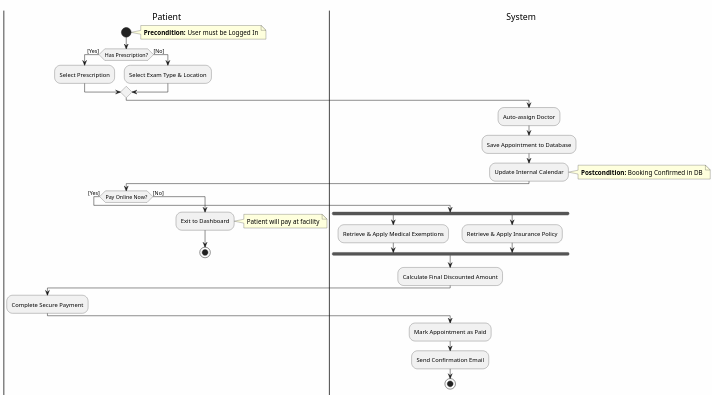
\includegraphics[width=0.8\textwidth]{Activity_Diagram/BookAppointments.png}
        \captionof{figure}{Activity Diagram for Book Appointment}
    \end{center}
    \begin{itemize}
        \item \textbf{Using:}
        \hyperlink{UC25}{Automated Doctor assignment}, 
        \hyperlink{UC27}{Appointment booking}, 
        \hyperlink{UC32}{Payment management}, \hyperlink{UC33}{Exemption application during payment},
        \hyperlink{UC34}{Insurance application during payment},
        \hyperlink{UC35}{Automatic appointment booking from prescription}
    \end{itemize}
\end{minipage}
\vspace{3em}

% --- BUNDLE 2 ---
\begin{minipage}{\textwidth}
    \subsection{2. Calendar Management}
    Here there's the entire flow of the management of a calendar.
    \begin{center}
        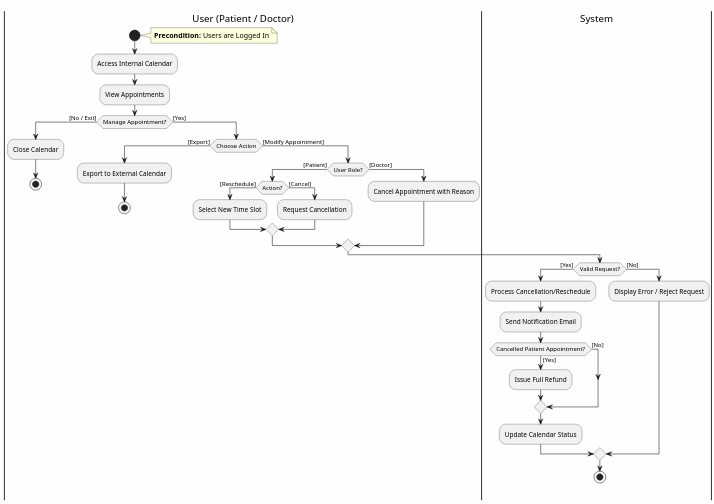
\includegraphics[width=0.8\textwidth]{Activity_Diagram/CalandarManagement.png}
        \captionof{figure}{Activity Diagram for Calendar Management}
    \end{center}
    \begin{itemize}
        \item \textbf{Using:}
        \hyperlink{UC28}{Patient appointment view},
        \hyperlink{UC10}{Patient appointment cancellation},
        \hyperlink{UC29}{Patient appointment rescheduling},
        \hyperlink{UC30}{Internal calendar integration},
        \hyperlink{UC45}{HoD appointment view}, \hyperlink{UC11}{Hospital staff appointment cancellation}
    \end{itemize}
\end{minipage}
\vspace{3em}

% --- BUNDLE 3 ---
\begin{minipage}{\textwidth}
    \subsection{3. Admin Actions}
    Here the flow of all the admin's possible actions.
    \begin{center}
        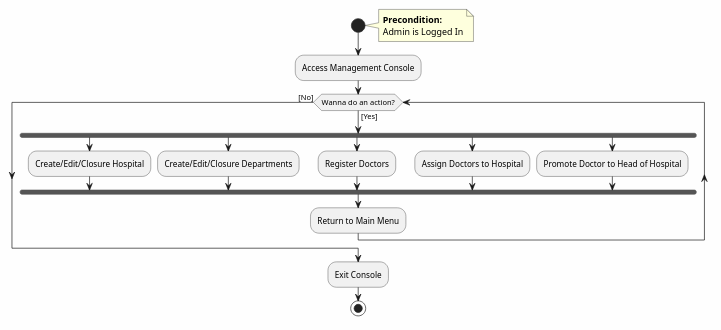
\includegraphics[width=0.8\textwidth]{Activity_Diagram/AdminActions.png}
        \captionof{figure}{Activity Diagram for Admin Actions}
    \end{center}
    \begin{itemize}
        \item \textbf{Using:}
        \hyperlink{UC1}{Hospital and Department creation},
        \hyperlink{UC5}{Hospital and Department edit},
        \hyperlink{UC8}{Hospital and Department closure},
        \hyperlink{UC12}{Doctor registration},
        \hyperlink{UC13}{Doctor assignment to a hospital},
        \hyperlink{UC14}{Promote Doctor to HoH}
    \end{itemize}
\end{minipage}
\vspace{3em}

% --- BUNDLE 4 ---
\begin{minipage}{\textwidth}
    \subsection{4. Head of Hospital Actions}
    Here there's the entire flow of all the Head of Hospital's possible actions.
    \begin{center}
        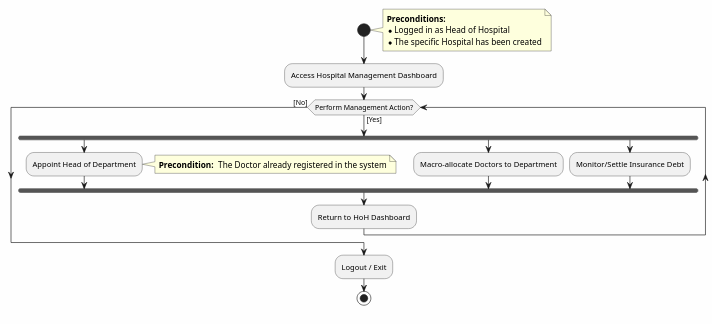
\includegraphics[width=0.8\textwidth]{Activity_Diagram/HeadOfHospitalActions.png}
        \captionof{figure}{Activity Diagram for Head of Hospital Actions}
    \end{center}
    \begin{itemize}
        \item \textbf{Using:} 
        \hyperlink{UC15}{Appoint HoD}, 
        \hyperlink{UC16}{Macro-allocate Doctors to Deparments},
        \hyperlink{UC18}{Insurance debt tracking and reporting},
        \hyperlink{UC19}{Insurance debt History},
        \hyperlink{UC20}{Manual settlement of insurance debt}
    \end{itemize}
\end{minipage}
\vspace{3em}

% --- BUNDLE 5 ---
\begin{minipage}{\textwidth}
    \subsection{5. Head of Department Actions}
    Here there's the entire flow of all the Head of Department's possible actions.
    \begin{center}
        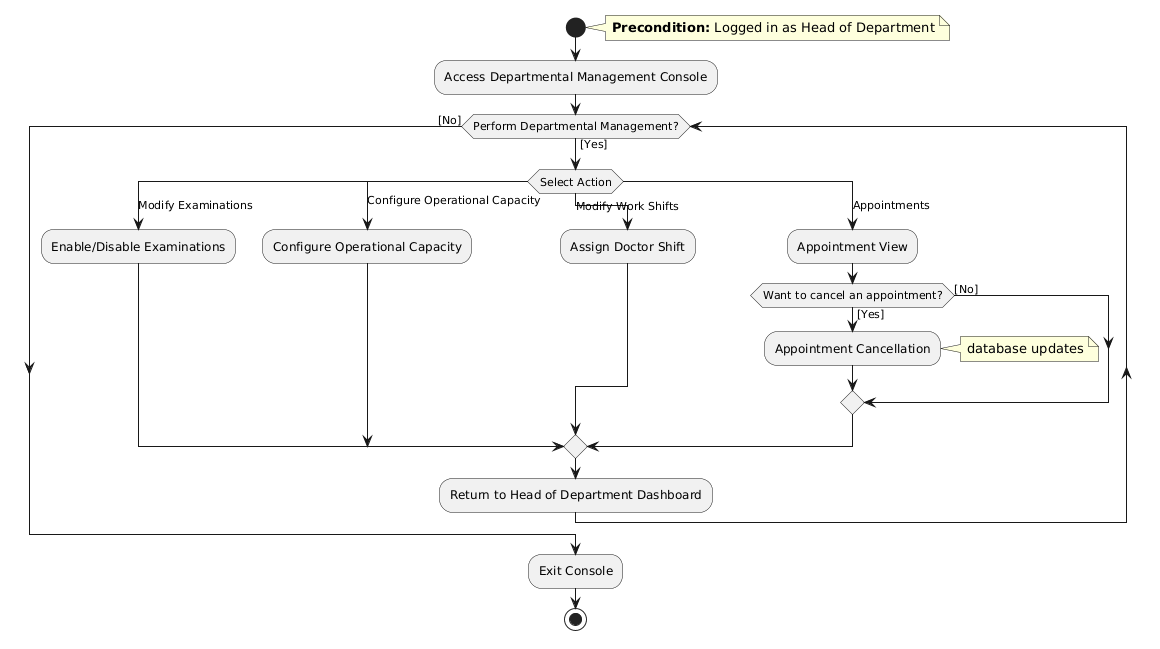
\includegraphics[width=0.8\textwidth]{Activity_Diagram/HeadOfDepartmentActions.png}
        \captionof{figure}{Activity Diagram for Head of Department Actions}
    \end{center}
    \begin{itemize}
        \item \textbf{Using:} 
        \hyperlink{UC17}{Enable/Disable Examinations},
        \hyperlink{UC21}{Configure Operational Capacity},
        \hyperlink{UC44}{Assign Doctor Shift},
        \hyperlink{UC28}{Appointment View},
        \hyperlink{UC11}{Appointment Cancellation}
    \end{itemize}
\end{minipage}
\vspace{3em}

% --- BUNDLE 6 ---
\begin{minipage}{\textwidth}
    \subsection{6. Doctor Operations}
    Here's the flow of the Doctor's action to manage the their Patients' account (exemptions/examinations/prescriptions).
    \begin{center}
        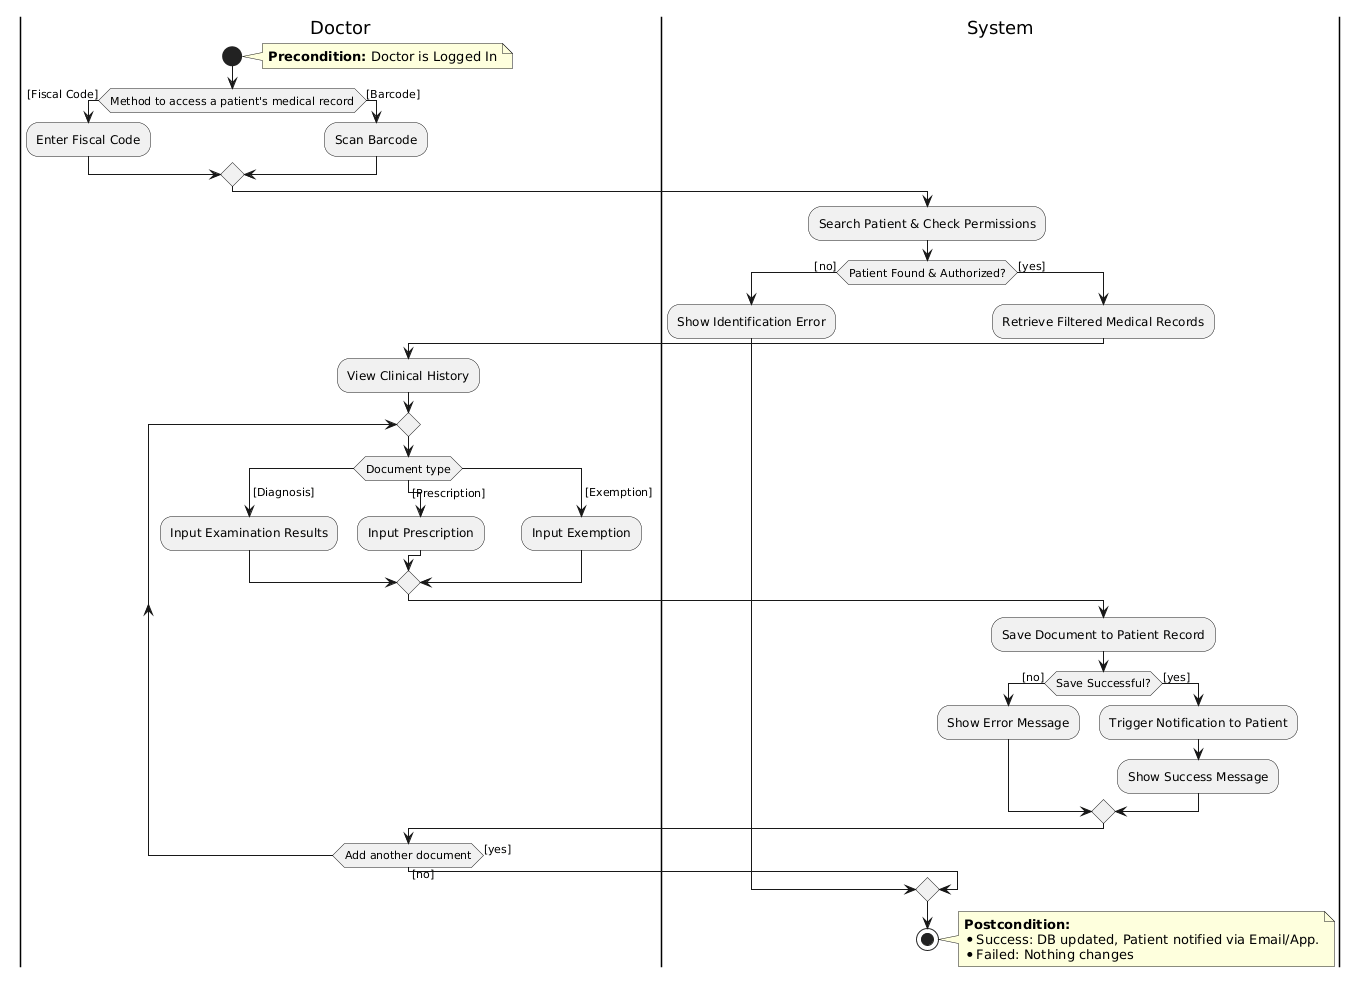
\includegraphics[width=0.8\textwidth]{Activity_Diagram/DoctorOperations.png}
        \captionof{figure}{Activity Diagram for Doctor Operations}
    \end{center}
    \begin{itemize}
        \item \textbf{Using:} 
        \hyperlink{UC42}{Access Medical Record via CF or Scan},
        \hyperlink{UC3}{Insert Prescription},
        \hyperlink{UC4}{Insert Diagnosis},
        \hyperlink{UC3}{Insert Exemption}
    \end{itemize}
\end{minipage}

% --- BUNDLE 7 ---
\begin{minipage}{\textwidth}
    \subsection{7. Account Lifecycle}
    Here's the activity flow of all the action related to the creation/management/deletion of an user account (which can be Doctors or Patients).
    \begin{center}
        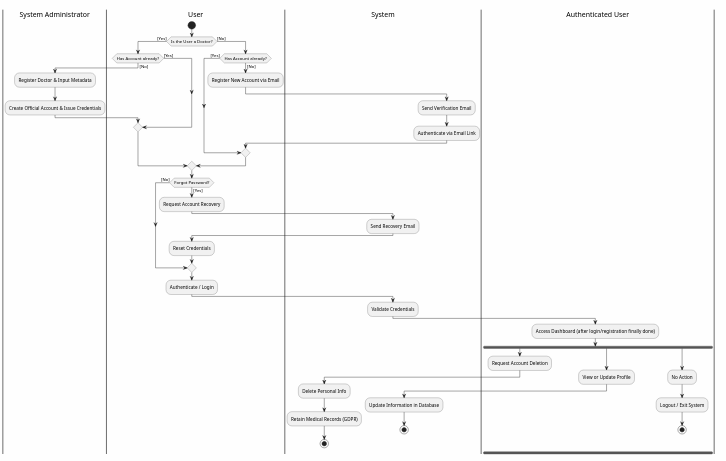
\includegraphics[width=0.8\textwidth]{Activity_Diagram/AccountLifecycle.png}
        \captionof{figure}{Activity Diagram for Account Lifecycle}
    \end{center}
    \begin{itemize}
        \item \textbf{Using:}
        \hyperlink{UC12}{Doctor Registration},
        \hyperlink{UC23}{User Registration and Authentication via Email},
        \hyperlink{UC26}{Password Recover},
        \hyperlink{UC24}{Login},
        \hyperlink{UC41}{Delete Account},
        \hyperlink{UC7}{Update Account}
    \end{itemize}
\end{minipage}

\section{Sequence Diagram}

% --- BUNDLE 1 ---
\begin{minipage}{\textwidth}
    \subsection{1. Reschedule Appointment}
    Here there's the sequence diagram of the reschedule of an appointment.
    \begin{center}
        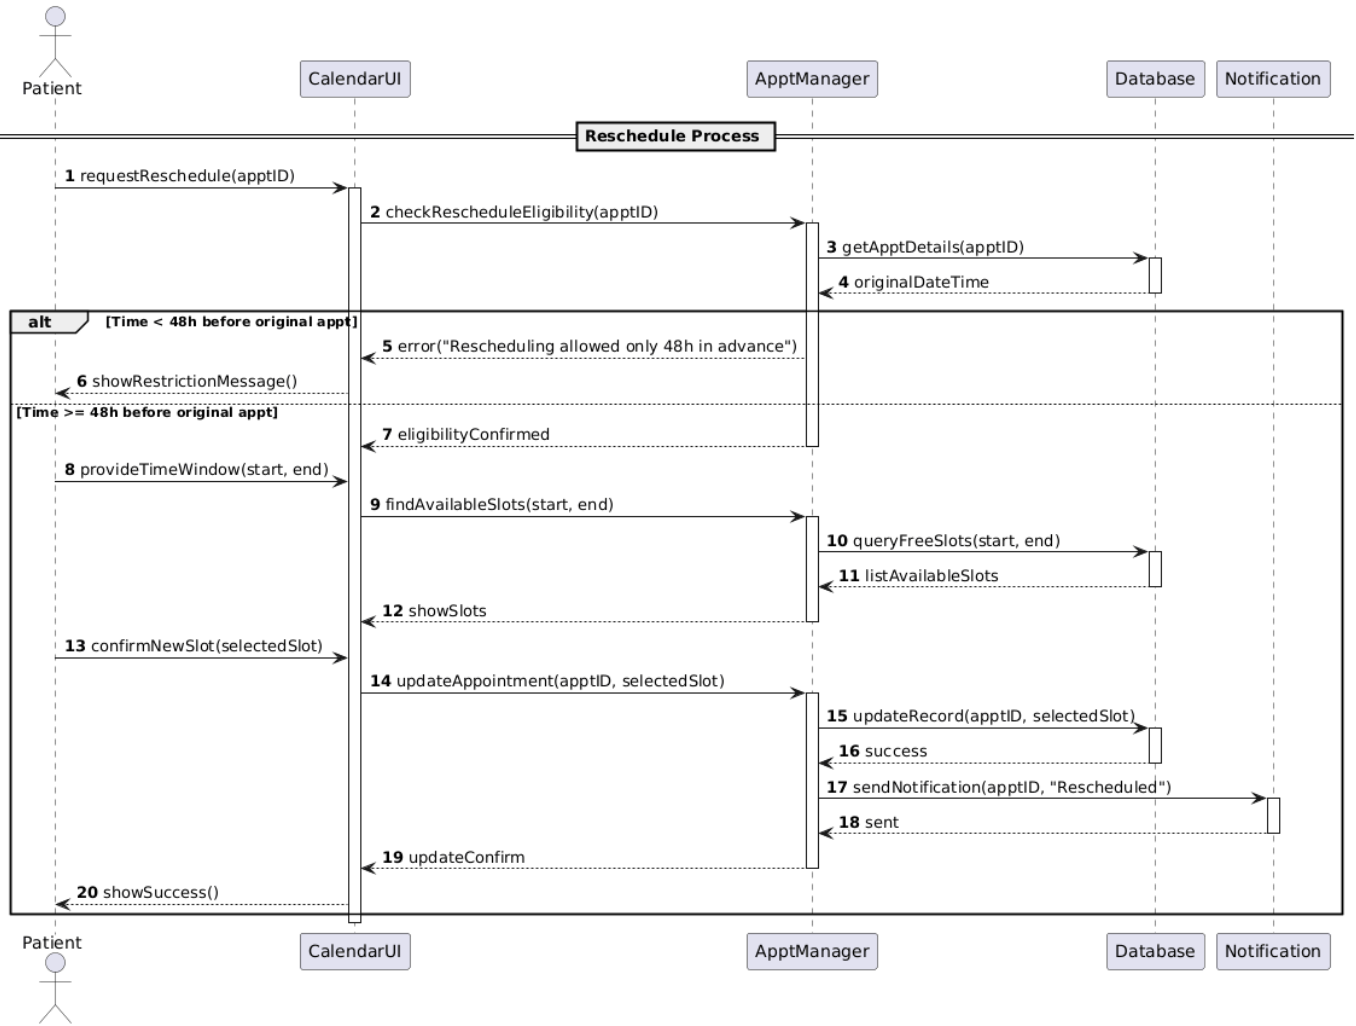
\includegraphics[width=0.8\textwidth]{Sequence_Diagram/RescheduleAppointment.png}
        \captionof{figure}{Sequence Diagram for Reschedule Appointment}
    \end{center}
    \begin{itemize}
        \item \textbf{Using:} 
        \hyperlink{UC29}{Patient Appointment Rescheduling}
    \end{itemize}
\end{minipage}
\vspace{3em}

% --- BUNDLE 2 ---
\begin{minipage}{\textwidth}
    \subsection{2. Cancel Appointment}
    Here is the sequence diagram of the cancel of an appointment, from both Patient or hospital staff point of view.
    \begin{center}
        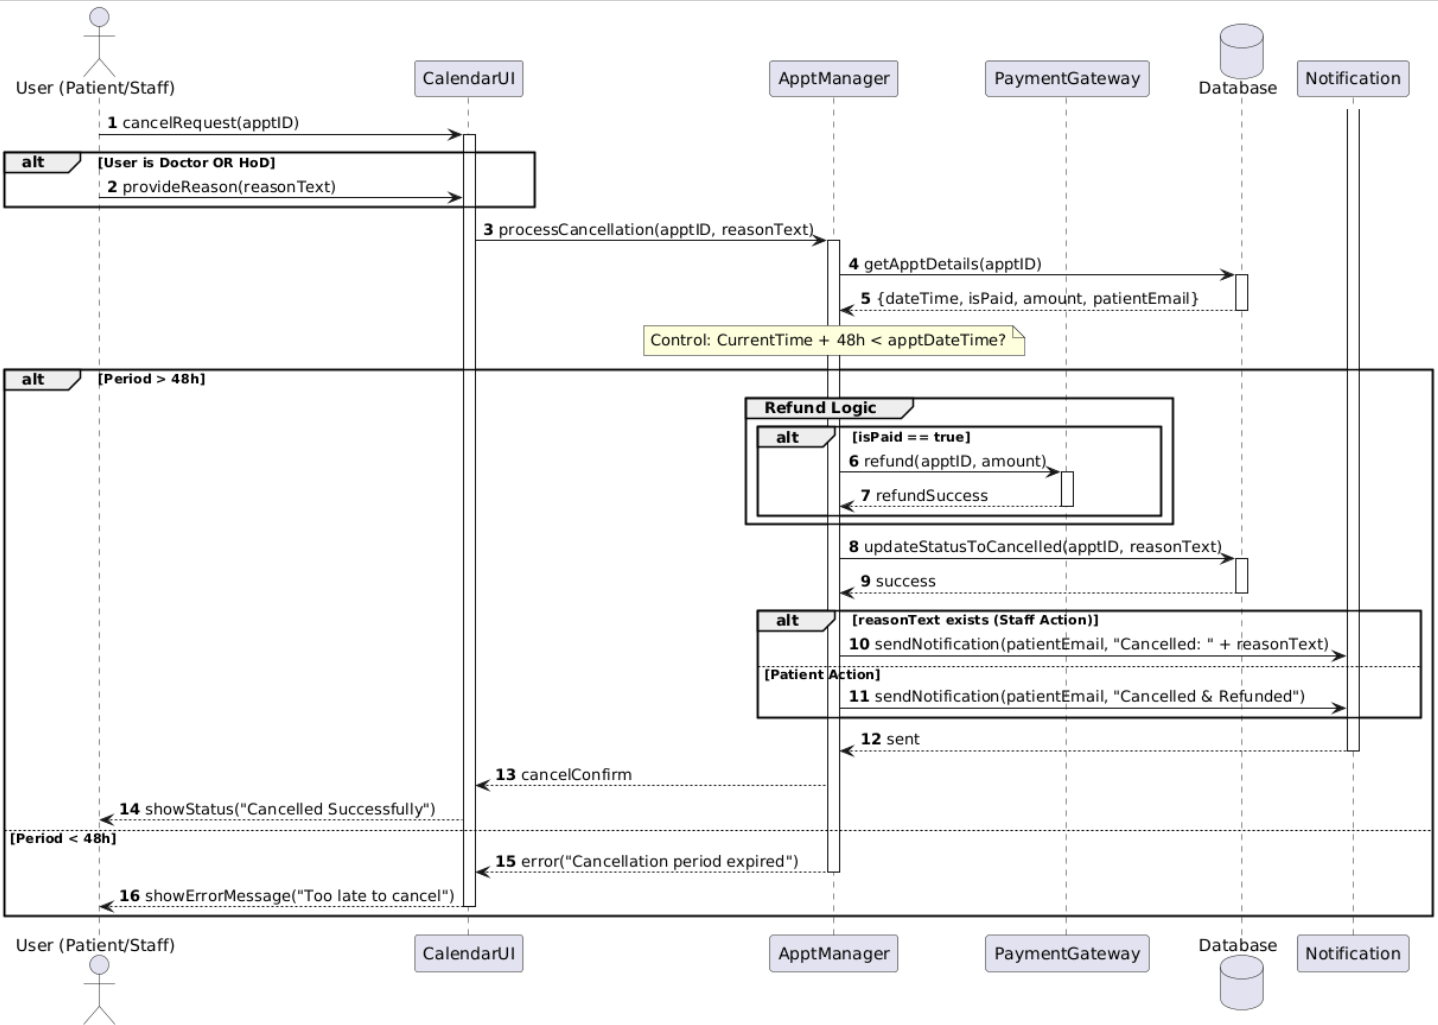
\includegraphics[width=0.8\textwidth]{Sequence_Diagram/CancelAppointment.png}
        \captionof{figure}{Sequence Diagram for Cancel Appointment}
    \end{center}
    \begin{itemize}
        \item \textbf{Using:} 
        \hyperlink{UC10}{Patient cancel appointment},
        \hyperlink{UC11}{Hospital staff cancel appointment}
    \end{itemize}
\end{minipage}
\vspace{3em}

% --- BUNDLE 3 ---
\begin{minipage}{\textwidth}
    \subsection{3. Doctor Upload Document}
    Here is the sequence activity related to the upload of documents by Doctor into the Patient's medical record.
    \begin{center}
        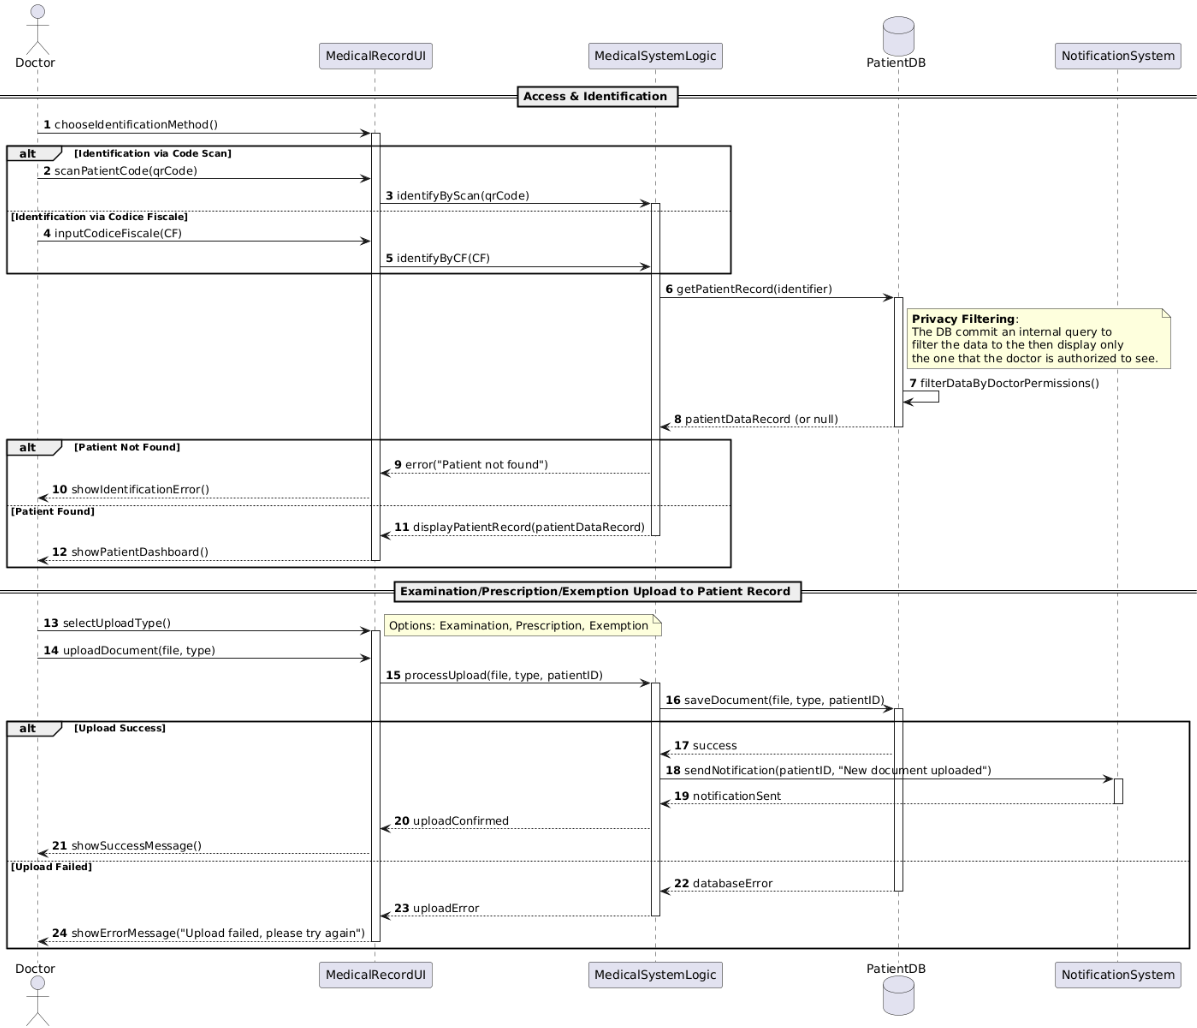
\includegraphics[width=0.8\textwidth]{Sequence_Diagram/DoctorUploadDocument.png}
        \captionof{figure}{Sequence Diagram for Doctor Upload Document}
    \end{center}
    \begin{itemize}
        \item \textbf{Using:} 
        \hyperlink{UC42}{Access Medical Record via CF or Scan},
        \hyperlink{UC3}{Insert Prescription},
        \hyperlink{UC4}{Insert Diagnosis},
        \hyperlink{UC3}{Insert Exemption}
    \end{itemize}
\end{minipage}
\vspace{3em}

% --- BUNDLE 4 ---
\begin{minipage}{\textwidth}
    \subsection{4. Registration User}
    Here is the sequence diagram about the registration of an user (that can be either a Doctor or a Patient).
    \begin{center}
        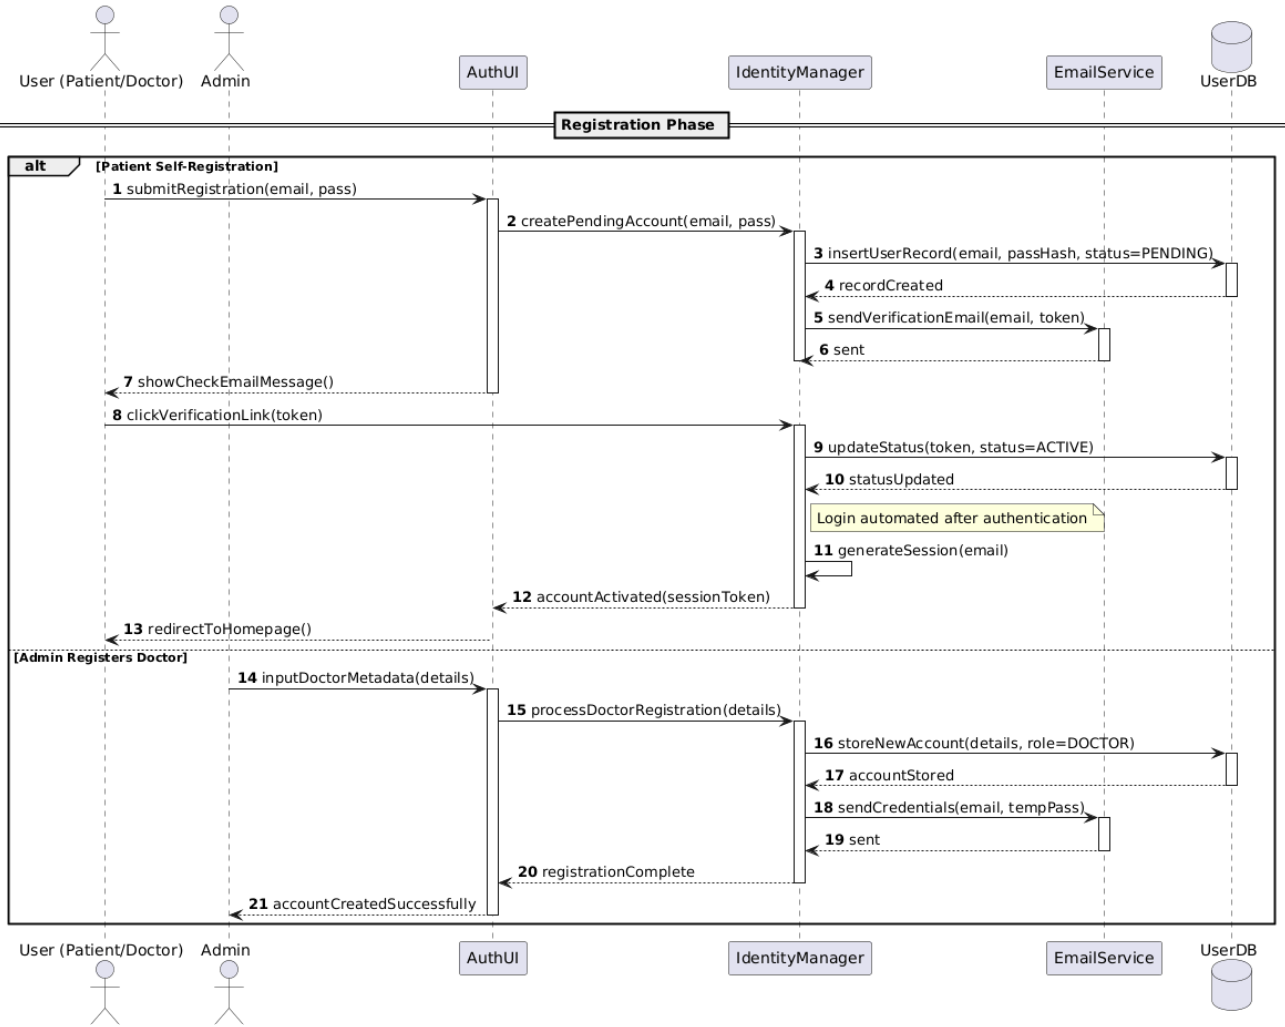
\includegraphics[width=0.8\textwidth]{Sequence_Diagram/RegistrationUser.png}
        \captionof{figure}{Sequence Diagram for Registration User}
    \end{center}
    \begin{itemize}
        \item \textbf{Using:} 
        \hyperlink{UC12}{Doctor Registration},
        \hyperlink{UC23}{User Registration and Authentication via Email}
    \end{itemize}
\end{minipage}
\vspace{3em}


% --- BUNDLE 5 ---
\begin{minipage}{\textwidth}
    \subsection{5. Book Appointment}
    Here the sequence diagram about the book of an appointment by a Patient.
    \begin{center}
        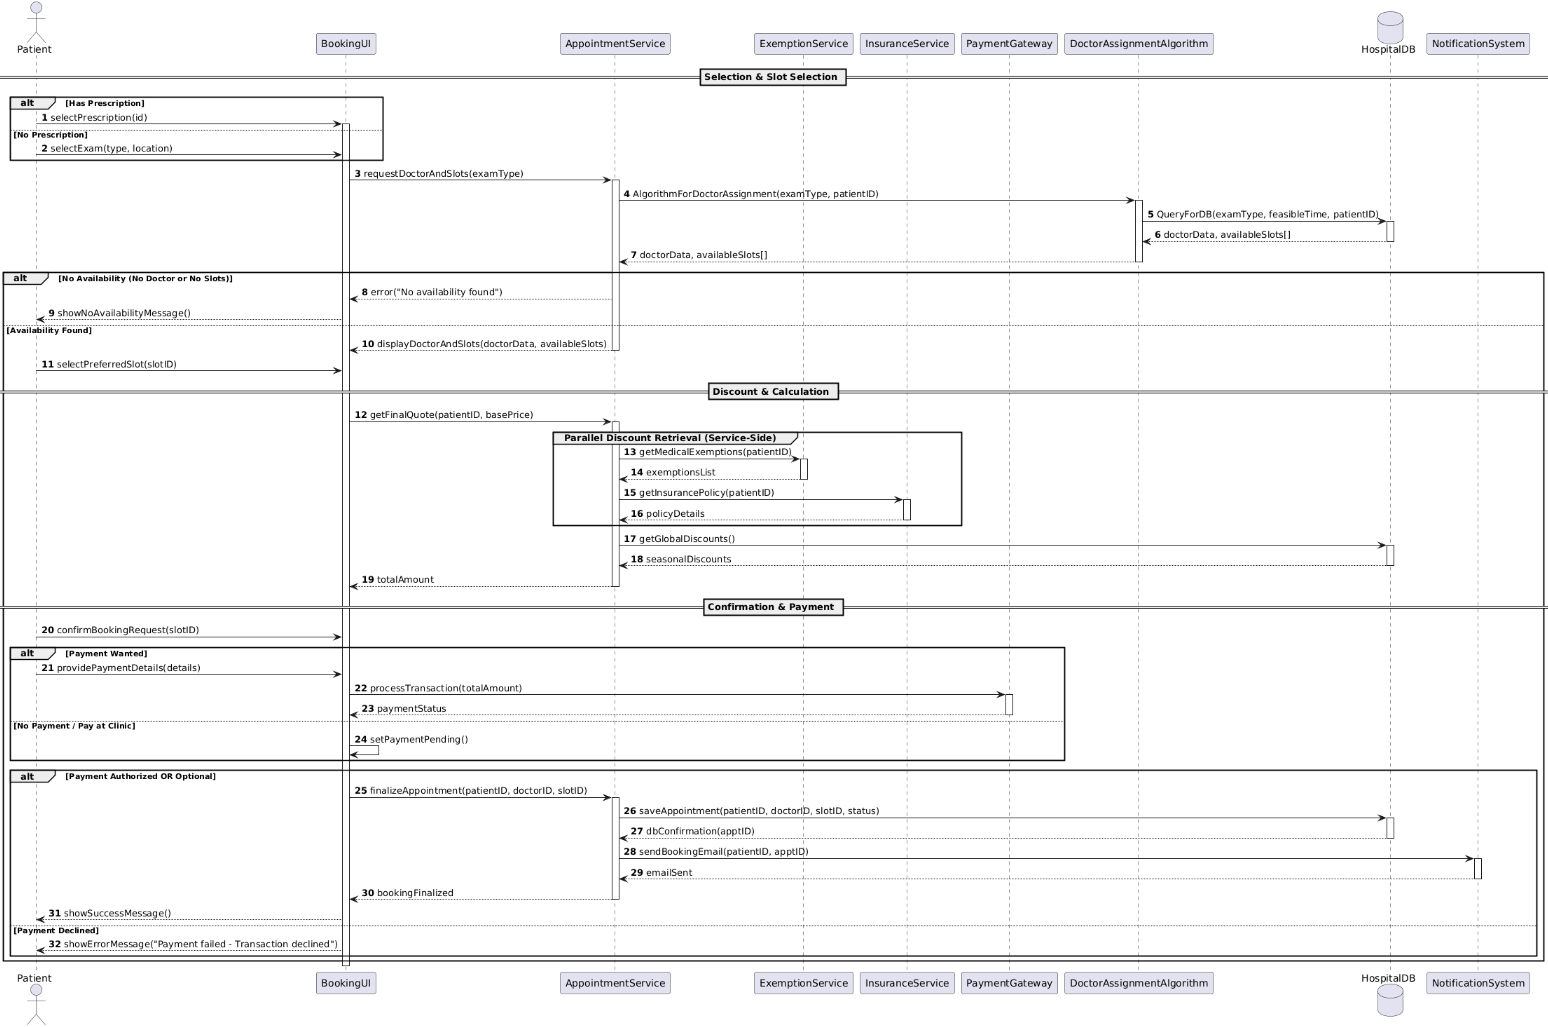
\includegraphics[width=0.8\textwidth]{Sequence_Diagram/BookAppointment.png}
        \captionof{figure}{Sequence Diagram for Book Appointment}
    \end{center}
    \begin{itemize}
        \item \textbf{Using:} 
        \hyperlink{UC25}{Automated Doctor assignment}, 
        \hyperlink{UC27}{Appointment booking}, 
        \hyperlink{UC32}{Payment management}, \hyperlink{UC33}{Exemption application during payment},
        \hyperlink{UC34}{Insurance application during payment},
        \hyperlink{UC35}{Automatic appointment booking from prescription}
    \end{itemize}
\end{minipage}
\vspace{3em}


% --- BUNDLE 6 ---
\begin{minipage}{\textwidth}
    \subsection{6. Account Login and Password Recovery}
    Here is the sequence diagram about the password recovery, that need the context of the user login, so we decided to implement them in a unique sequence diagram.
    \begin{center}
        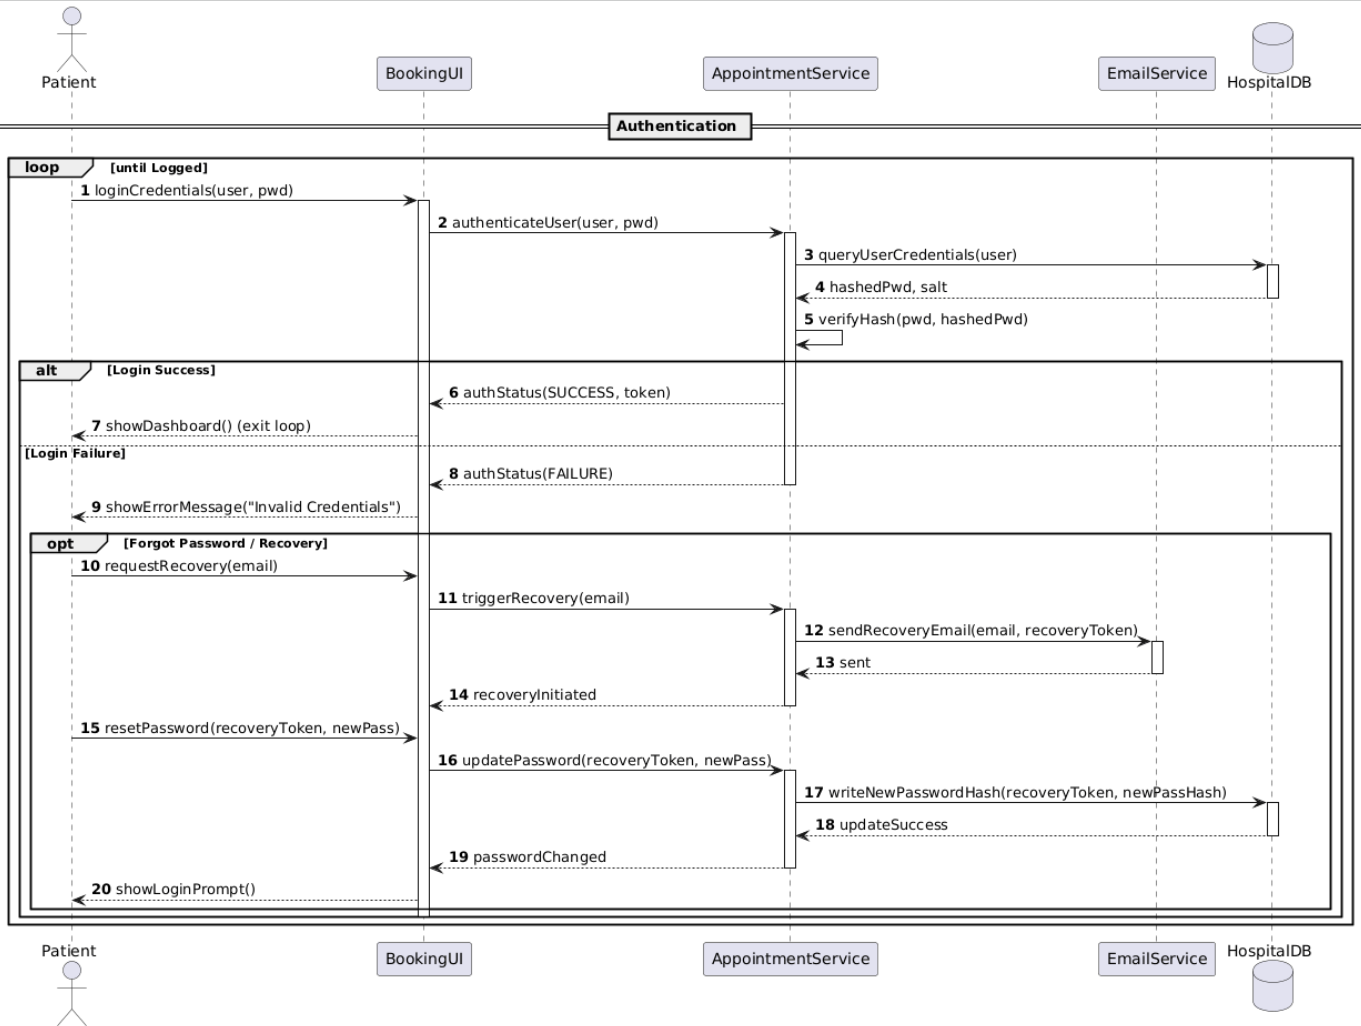
\includegraphics[width=0.8\textwidth]{Sequence_Diagram/LoginUserAndRecovery.png}
        \captionof{figure}{Sequence Diagram for Login and Password Recovery}
    \end{center}
    \begin{itemize}
        \item \textbf{Using:} 
        \hyperlink{UC26}{Password Recover},
        \hyperlink{UC24}{Login}
    \end{itemize}
\end{minipage}
\vspace{3em}


% --- BUNDLE 7 ---
\begin{minipage}{\textwidth}
    \subsection{7. Account Management}
    Here the sequence diagram about the operations related to the edit and deletion of an user account (that can be either a Doctor or a Patient).
    \begin{center}
        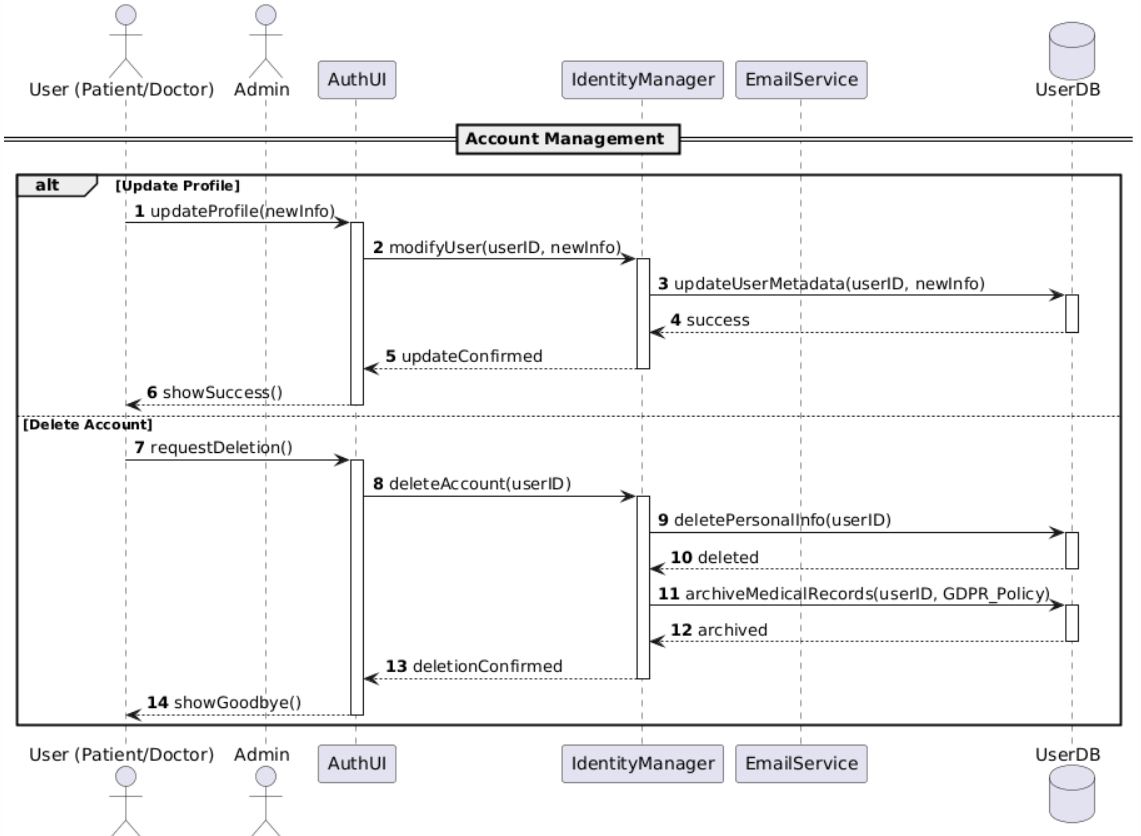
\includegraphics[width=0.8\textwidth]{Sequence_Diagram/AccountManagement.png}
        \captionof{figure}{Sequence Diagram for Account Management Operations}
    \end{center}
    \begin{itemize}
        \item \textbf{Using:} 
        \hyperlink{UC41}{Delete Account},
        \hyperlink{UC7}{Update Account}
    \end{itemize}
\end{minipage}
\vspace{3em}


\section{Class Diagram}
For readability purposes, the class diagram has been attached separately as a PDF document.

\subsection{1. HealthMaxxinSystem}\label{sec:1-healthmaxxinsystem}

\textbf{Description}

The central singleton class representing the entire HealthMaxxing platform. It acts as the top-level container and entry point for the system, tying together the major subsystems: the hospital network, the user base, the treatment catalog, and insurance policies. Its existence ensures that all components operate within a single, coherent system context.

\textbf{Attributes}

\begin{center}
\small
\renewcommand{\arraystretch}{1.35}
\begin{tabularx}{\textwidth}{|>{\raggedright\arraybackslash}p{3.4cm}|>{\raggedright\arraybackslash}p{3.3cm}|Y|}
\hline
\rowcolor{gray!20}
\textbf{Attribute} & \textbf{Type} & \textbf{Description} \\ \hline
\texttt{systemName} & String & The display name of the platform \\ \hline
\texttt{version} & String & The current running version of the software \\ \hline
\end{tabularx}
\end{center}

\textbf{Relationships}

\begin{itemize}
    \item Contains (1-to-1) one \texttt{SystemAdmin, User, Hospital, TreatmentCatalog, InsurancePolicy and mail Service} as the core components of the system
\end{itemize}

\par\medskip\hrule\medskip

\subsection{2. User}\label{sec:2-user}

\textbf{Description}

The base class for all human actors who interact with the HealthMaxxing platform (excluding \texttt{SystemAdmin}, which is a separate administrative entity). It encapsulates the shared identity and authentication data common to all user roles, patients, doctors, department heads, and hospital heads. Every user has a unique account, can authenticate, and can manage their own profile. 

\textbf{Attributes}

\begin{center}
\small
\renewcommand{\arraystretch}{1.35}
\begin{tabularx}{\textwidth}{|>{\raggedright\arraybackslash}p{3.4cm}|>{\raggedright\arraybackslash}p{3.3cm}|Y|}
\hline
\rowcolor{gray!20}
\textbf{Attribute} & \textbf{Type} & \textbf{Description} \\ \hline
\texttt{id} & String & Unique identifier for the user \\ \hline
\texttt{firstName} & String & The user's first name \\ \hline
\texttt{lastName} & String & The user's last name \\ \hline
\texttt{email} & String & The user's email address, used for login and notifications \\ \hline
\texttt{fiscalCode} & String & Italian tax code, used as a universal health identifier \\ \hline
\texttt{passwordHash} & String & Hashed version of the user's password \\ \hline
\texttt{isVerified} & Boolean & Whether the user's email address has been verified \\ \hline
\texttt{createdAt} & DateTime & Timestamp of account creation \\ \hline
\end{tabularx}
\end{center}

\textbf{Methods}

\begin{center}
\small
\renewcommand{\arraystretch}{1.35}
\begin{tabularx}{\textwidth}{|M|Y|}
\hline
\rowcolor{gray!20}
\textbf{Method} & \textbf{Description} \\ \hline
\texttt{login()} & Authenticates the user and initiates a session \\ \hline
\texttt{logout()} & Terminates the active session \\ \hline
\texttt{viewProfile()} & Returns the user's profile information \\ \hline
\texttt{updateProfile()} & Allows the user to modify their personal details \\ \hline
\texttt{requestPasswordReset()} & Triggers a password reset flow (email with temporary credentials) \\ \hline
\texttt{deleteAccount()} & Permanently removes the user account from the system \\ \hline
\end{tabularx}
\end{center}

\textbf{Relationships}

\begin{itemize}
    \item Superclass of \texttt{Patient}, \texttt{Doctor}, \texttt{HeadOfDepartment}, and \texttt{HeadOfHospital}
    \item Owns exactly one \texttt{Calendar}
    \item May have zero or one \texttt{TemporaryPassword} at any given time
    \item Is notified by \texttt{MailService} for account-related events
\end{itemize}

\par\medskip\hrule\medskip

\subsection{3. Patient}\label{sec:3-patient}

\textbf{Description}


A specialization of \texttt{User} representing individuals who seek and receive medical care within the system. Patients are the primary consumers of healthcare services: they book appointments for treatments, manage their insurance coverage, and accumulate a health history.

\textbf{Attributes}

\begin{center}
\small
\renewcommand{\arraystretch}{1.35}
\begin{tabularx}{\textwidth}{|>{\raggedright\arraybackslash}p{3.4cm}|>{\raggedright\arraybackslash}p{3.3cm}|Y|}
\hline
\rowcolor{gray!20}
\textbf{Attribute} & \textbf{Type} & \textbf{Description} \\ \hline
\texttt{address} & String & The patient's residential address \\ \hline
\texttt{dateOfBirth} & Date & The patient's date of birth \\ \hline
\end{tabularx}
\end{center}

\emph{(Inherits all attributes from \texttt{User})}

\textbf{Methods}

\begin{center}
\small
\renewcommand{\arraystretch}{1.35}
\begin{tabularx}{\textwidth}{|M|Y|}
\hline
\rowcolor{gray!20}
\textbf{Method} & \textbf{Description} \\ \hline
\texttt{bookAppointment()} & Creates a new appointment request for a treatment \\ \hline
\texttt{cancelAppointment()} & Cancels an existing appointment \\ \hline
\texttt{rescheduleAppointment()} & Moves an existing appointment to a new date/time \\ \hline
\texttt{registerInsurance(code: String)} & Links an insurance policy to the patient's profile using a unique code \\ \hline
\end{tabularx}
\end{center}

\textbf{Relationships}

\begin{itemize}
    \item Is assisted by exactly one \texttt{AiAssistant}
    \item Is the "Booked By" party for \texttt{Appointment} (1 patient to 0..N appointments)
    \item Receives \texttt{Prescription} records (issued to 0..N)
    \item Holds \texttt{Exemption} records (belongs to 0..N)
    \item Holds \texttt{Examination} records (issued to 0..N)
    \item Linked to \texttt{InsurancePolicyRecord} entries (0..N)
\end{itemize}

\par\medskip\hrule\medskip

\subsection{4. Doctor}\label{sec:4-doctor}

\textbf{Description}

A specialization of \texttt{User} representing licensed medical professionals registered in the system. Doctors are the primary healthcare providers: they conduct appointments, issue prescriptions and exemptions, upload examination results, and access patient records. They are assigned to one or more departments and operate according to scheduled shifts. Doctors form the basis for the more privileged \texttt{HeadOfDepartment} and \texttt{HeadOfHospital} roles.

\textbf{Attributes}

\begin{center}
\small
\renewcommand{\arraystretch}{1.35}
\begin{tabularx}{\textwidth}{|>{\raggedright\arraybackslash}p{3.4cm}|>{\raggedright\arraybackslash}p{3.3cm}|Y|}
\hline
\rowcolor{gray!20}
\textbf{Attribute} & \textbf{Type} & \textbf{Description} \\ \hline
\texttt{specialty} & String & The medical specialty of the doctor (e.g., Cardiology, Radiology) \\ \hline
\end{tabularx}
\end{center}

\emph{(Inherits all attributes from \texttt{User})}

\textbf{Methods}

\begin{center}
\small
\renewcommand{\arraystretch}{1.35}
\begin{tabularx}{\textwidth}{|M|Y|}
\hline
\rowcolor{gray!20}
\textbf{Method} & \textbf{Description} \\ \hline
\texttt{viewAppointments()} & Retrieves the list of appointments assigned to this doctor \\ \hline
\texttt{cancelAppointment(reason: String)} & Cancels an appointment and records the reason \\ \hline
\texttt{createPrescription()} & Issues a new prescription for a patient \\ \hline
\texttt{createExemption()} & Issues a new exemption record for a patient \\ \hline
\texttt{accessPatientRecord(fiscalCode: String)} & Looks up a patient's full medical history using their fiscal code \\ \hline
\texttt{uploadExamination()} & Attaches examination results to a patient's record \\ \hline
\texttt{viewChronologicalReport()} & Generates a chronological view of all clinical activities \\ \hline
\end{tabularx}
\end{center}

\textbf{Relationships}

\begin{itemize}
    \item Works at a \texttt{Department} (0..1 department at a time)
    \item Assigned to \texttt{Appointment} records (0..N)
    \item Issues \texttt{Prescription} records (0..N)
    \item Creates \texttt{Exemption} records (0..N)
    \item Schedules follow a \texttt{Shift} pattern (0..N)
    \item Is notified by \texttt{MailService} for shift changes and credentials
\end{itemize}

\par\medskip\hrule\medskip

\subsection{5. HeadOfDepartment}\label{sec:5-headofdepartment}

\textbf{Description}

A specialization of \texttt{Doctor} with additional administrative authority scoped to a single department. The Head of Department oversees the operational management of their unit: they configure capacity, define treatment offerings, manage doctor assignments, and maintain shift patterns. They also have visibility into all appointments occurring within their department and can intervene by cancelling them when necessary.

\textbf{Methods}

\begin{center}
\small
\renewcommand{\arraystretch}{1.35}
\begin{tabularx}{\textwidth}{|M|Y|}
\hline
\rowcolor{gray!20}
\textbf{Method} & \textbf{Description} \\ \hline
\texttt{assignDoctorToDepartment()} & Assigns a doctor to work within this department \\ \hline
\texttt{updateDepartmentTreatments()} & Modifies the list of treatments offered by the department \\ \hline
\texttt{configureDepartmentCapacity()} & Sets or updates the maximum patient capacity for the department \\ \hline
\texttt{setShiftPattern(doctor: Doctor)} & Defines or updates the work shift schedule for a specific doctor \\ \hline
\texttt{viewDepartmentAppointments()} & Retrieves all appointments booked within the department \\ \hline
\texttt{cancelDepartmentAppointment(reason: String)} & Cancels an appointment at the department level with a stated reason \\ \hline
\end{tabularx}
\end{center}

\emph{(Inherits all attributes and methods from \texttt{Doctor} and \texttt{User})}

\textbf{Relationships}

\begin{itemize}
    \item Manages exactly one \texttt{Department} (1-to-1)
    \item Manages doctor schedules via \texttt{Shift} associations
\end{itemize}

\par\medskip\hrule\medskip

\subsection{6. HeadOfHospital}\label{sec:6-headofhospital}

\textbf{Description}

A specialization of \texttt{Doctor} with the highest level of administrative authority within a specific hospital. The Head of Hospital oversees the appointment and allocation of staff at the departmental and hospital-wide level. They are also the key actor in financial management, having visibility into insurance-related debts and the ability to settle outstanding balances with insurance companies.

\textbf{Methods}

\begin{center}
\small
\renewcommand{\arraystretch}{1.35}
\begin{tabularx}{\textwidth}{|M|Y|}
\hline
\rowcolor{gray!20}
\textbf{Method} & \textbf{Description} \\ \hline
\texttt{appointHeadOfDepartment(doctor: Doctor, dept: Department)} & Designates a doctor as the Head of a specific department \\ \hline
\texttt{allocateDoctors(doctors: List<Doctor>, dept: Department)} & Assigns a group of doctors to a department \\ \hline
\texttt{viewInsuranceDebt()} & Displays the outstanding debt owed by insurance companies \\ \hline
\texttt{settleInsuranceDebt(company: InsuranceCompany, amount: Decimal)} & Records a partial or full debt settlement with an insurance company \\ \hline
\end{tabularx}
\end{center}

\emph{(Inherits all attributes and methods from \texttt{Doctor} and \texttt{User})}

\textbf{Relationships}

\begin{itemize}
    \item Manages exactly one \texttt{Hospital} (1-to-1)
    \item Interacts with \texttt{OutstandingDebt} to monitor and settle insurance balances
\end{itemize}

\par\medskip\hrule\medskip

\subsection{7. SystemAdmin}\label{sec:7-systemadmin}

\textbf{Description}

A privileged, platform-level administrator who sits outside the \texttt{User} hierarchy. The System Admin is responsible for the configuration and lifecycle management of the entire platform infrastructure: creating and closing hospitals and departments, registering doctors, and managing insurance policies and treatments globally. This role is typically held by platform operators rather than healthcare professionals and has no patient-facing responsibilities. It has its own separate authentication mechanism.

\textbf{Attributes}

\begin{center}
\small
\renewcommand{\arraystretch}{1.35}
\begin{tabularx}{\textwidth}{|>{\raggedright\arraybackslash}p{3.4cm}|>{\raggedright\arraybackslash}p{3.3cm}|Y|}
\hline
\rowcolor{gray!20}
\textbf{Attribute} & \textbf{Type} & \textbf{Description} \\ \hline
\texttt{id} & UUID & Unique identifier for the admin account \\ \hline
\texttt{username} & String & The login username \\ \hline
\texttt{passwordHash} & String & Hashed password for admin authentication \\ \hline
\end{tabularx}
\end{center}

\textbf{Methods}

\begin{center}
\small
\renewcommand{\arraystretch}{1.35}
\begin{tabularx}{\textwidth}{|M|Y|}
\hline
\rowcolor{gray!20}
\textbf{Method} & \textbf{Description} \\ \hline
\texttt{createHospital()} & Registers a new hospital in the system \\ \hline
\texttt{editHospital()} & Updates hospital details \\ \hline
\texttt{closeHospital()} & Marks a hospital as closed and inactive \\ \hline
\texttt{createDepartment()} & Creates a new department within a hospital \\ \hline
\texttt{editDepartment()} & Modifies department attributes \\ \hline
\texttt{closeDepartment()} & Deactivates a department \\ \hline
\texttt{registerDoctor()} & Adds a new doctor to the platform \\ \hline
\texttt{assignDoctorToHospital()} & Associates a doctor with a specific hospital \\ \hline
\texttt{appointHeadOfHospital(doctor: Doctor, hospital: Hospital)} & Designates a doctor as the Head of a Hospital \\ \hline
\texttt{createInsurancePolicy()} & Adds a new insurance policy to the system \\ \hline
\texttt{editInsurancePolicy()} & Updates an existing insurance policy \\ \hline
\texttt{deactivateInsurancePolicy()} & Disables an insurance policy \\ \hline
\texttt{generateInsuranceCode(policy: InsurancePolicy, patient: Patient)} & Generates a unique insurance code linking a policy to a patient \\ \hline
\texttt{createTreatment()} & Adds a new treatment to the global catalog \\ \hline
\texttt{editTreatment()} & Modifies an existing treatment \\ \hline
\texttt{deactivateTreatment()} & Removes a treatment from active availability \\ \hline
\texttt{adminLogin()} & Authenticates the system administrator \\ \hline
\texttt{adminLogout()} & Terminates the admin session \\ \hline
\end{tabularx}
\end{center}

\textbf{Relationships}

\begin{itemize}
    \item Operates at the \texttt{HealthMaxxinSystem} level (1-to-1)
    \item Manages \texttt{Hospital}, \texttt{Department}, \texttt{Doctor}, \texttt{InsurancePolicy}, and \texttt{Treatment} lifecycle
\end{itemize}

\par\medskip\hrule\medskip

\subsection{8. Hospital}\label{sec:8-hospital}

\textbf{Description}

Represents a physical hospital facility registered within the platform. A hospital is the top-level organizational unit in the care delivery hierarchy, containing multiple departments and employing doctors. Its status lifecycle (active/closed) is managed by the \texttt{SystemAdmin}. Each hospital is headed by a \texttt{HeadOfHospital} and can accumulate insurance-related debt tracked via \texttt{OutstandingDebt}.

\textbf{Attributes}

\begin{center}
\small
\renewcommand{\arraystretch}{1.35}
\begin{tabularx}{\textwidth}{|>{\raggedright\arraybackslash}p{3.4cm}|>{\raggedright\arraybackslash}p{3.3cm}|Y|}
\hline
\rowcolor{gray!20}
\textbf{Attribute} & \textbf{Type} & \textbf{Description} \\ \hline
\texttt{id} & UUID & Unique identifier \\ \hline
\texttt{name} & String & Official name of the hospital \\ \hline
\texttt{address} & String & Physical address of the facility \\ \hline
\texttt{status} & HospitalStatus & Current operational status (e.g., ACTIVE, CLOSED) \\ \hline
\texttt{createdAt} & DateTime & Timestamp of registration in the system \\ \hline
\end{tabularx}
\end{center}

\textbf{Methods}

\begin{center}
\small
\renewcommand{\arraystretch}{1.35}
\begin{tabularx}{\textwidth}{|M|Y|}
\hline
\rowcolor{gray!20}
\textbf{Method} & \textbf{Description} \\ \hline
\texttt{close()} & Transitions the hospital to a closed state \\ \hline
\end{tabularx}
\end{center}

\textbf{Relationships}

\begin{itemize}
    \item Contains 1..N \texttt{Department} entities
    \item Managed by exactly one \texttt{HeadOfHospital}
    \item Owes debt tracked by \texttt{OutstandingDebt}
\end{itemize}

\par\medskip\hrule\medskip

\subsection{9. Department}\label{sec:9-department}

\textbf{Description}

Represents a specialized medical unit within a hospital (e.g., Cardiology, Oncology, Radiology). A department defines what treatments it offers, how many patients it can handle (capacity), and which doctors are working within it. Its operational state is managed through status flags, and it can be closed when no longer active. Departments are the direct context in which appointments and clinical activities take place.

\textbf{Attributes}

\begin{center}
\small
\renewcommand{\arraystretch}{1.35}
\begin{tabularx}{\textwidth}{|>{\raggedright\arraybackslash}p{3.4cm}|>{\raggedright\arraybackslash}p{3.3cm}|Y|}
\hline
\rowcolor{gray!20}
\textbf{Attribute} & \textbf{Type} & \textbf{Description} \\ \hline
\texttt{id} & UUID & Unique identifier \\ \hline
\texttt{name} & String & Name of the department (e.g., "Cardiology") \\ \hline
\texttt{capacity} & Integer & Maximum number of patients/appointments the department can handle \\ \hline
\texttt{status} & DepartmentStatus & Current operational status (e.g., ACTIVE, CLOSED) \\ \hline
\texttt{createdAt} & DateTime & Timestamp of creation \\ \hline
\end{tabularx}
\end{center}

\textbf{Methods}

\begin{center}
\small
\renewcommand{\arraystretch}{1.35}
\begin{tabularx}{\textwidth}{|M|Y|}
\hline
\rowcolor{gray!20}
\textbf{Method} & \textbf{Description} \\ \hline
\texttt{close()} & Transitions the department to a closed/inactive state \\ \hline
\end{tabularx}
\end{center}

\textbf{Relationships}

\begin{itemize}
    \item Belongs to exactly one \texttt{Hospital}
    \item Managed by exactly one \texttt{HeadOfDepartment}
    \item Offers 0..N \texttt{Treatment} types
    \item Houses 0..N \texttt{Doctor} workers
    \item Is the site of 0..N \texttt{Appointment} records
\end{itemize}

\par\medskip\hrule\medskip

\subsection{10. Shift}\label{sec:10-shift}

\textbf{Description}

Defines a recurring working time block for a specific doctor. A shift is characterized by a day of the week and a time window, and is valid within a defined date range. This allows the system to model part-time schedules, rotations, and temporary duty assignments. The validity check ensures the system only considers shifts that fall within their active period when computing doctor availability for appointment booking.

\textbf{Attributes}

\begin{center}
\small
\renewcommand{\arraystretch}{1.35}
\begin{tabularx}{\textwidth}{|>{\raggedright\arraybackslash}p{3.4cm}|>{\raggedright\arraybackslash}p{3.3cm}|Y|}
\hline
\rowcolor{gray!20}
\textbf{Attribute} & \textbf{Type} & \textbf{Description} \\ \hline
\texttt{id} & UUID & Unique identifier \\ \hline
\texttt{startTime} & Time & The time the shift begins \\ \hline
\texttt{endTime} & Time & The time the shift ends \\ \hline
\texttt{dayOfWeek} & DayOfWeek & The day of the week this shift applies to \\ \hline
\texttt{validFrom} & Date & Start date of this shift's validity period \\ \hline
\texttt{validUntil} & Date & End date of this shift's validity period \\ \hline
\end{tabularx}
\end{center}

\textbf{Methods}

\begin{center}
\small
\renewcommand{\arraystretch}{1.35}
\begin{tabularx}{\textwidth}{|M|Y|}
\hline
\rowcolor{gray!20}
\textbf{Method} & \textbf{Description} \\ \hline
\texttt{isValid()} & Returns true if the current date falls within the validFrom–validUntil range \\ \hline
\end{tabularx}
\end{center}

\textbf{Relationships}

\begin{itemize}
    \item Schedules 0..N \texttt{Doctor} working patterns (each doctor has 0..N shifts)
    \item Set by \texttt{HeadOfDepartment} via \texttt{setShiftPattern()}
\end{itemize}

\par\medskip\hrule\medskip

\subsection{11. Calendar}\label{sec:11-calendar}

\textbf{Description}

A personal scheduling container owned by each \texttt{User}. It aggregates all appointments associated with that user and provides a secure export mechanism for integration with external calendar applications (e.g., Google Calendar, iCal). The export is token-protected and time-limited to prevent unauthorized access.

\textbf{Attributes}

\begin{center}
\small
\renewcommand{\arraystretch}{1.35}
\begin{tabularx}{\textwidth}{|>{\raggedright\arraybackslash}p{3.4cm}|>{\raggedright\arraybackslash}p{3.3cm}|Y|}
\hline
\rowcolor{gray!20}
\textbf{Attribute} & \textbf{Type} & \textbf{Description} \\ \hline
\texttt{id} & UUID & Unique identifier \\ \hline
\texttt{exportToken} & String & A secure token for external calendar export/sync \\ \hline
\texttt{tokenExpiresAt} & DateTime & Expiry timestamp of the export token \\ \hline
\end{tabularx}
\end{center}

\textbf{Methods}

\begin{center}
\small
\renewcommand{\arraystretch}{1.35}
\begin{tabularx}{\textwidth}{|M|Y|}
\hline
\rowcolor{gray!20}
\textbf{Method} & \textbf{Description} \\ \hline
\texttt{generateExportToken()} & Creates or refreshes the export token with a new expiry date \\ \hline
\texttt{getAppointments()} & Returns the list of all appointments associated with this calendar \\ \hline
\end{tabularx}
\end{center}

\textbf{Relationships}

\begin{itemize}
    \item Owned by exactly one \texttt{User} (1-to-1)
    \item Displays 0..N \texttt{Appointment} records
\end{itemize}

\par\medskip\hrule\medskip

\subsection{12. TemporaryPassword}\label{sec:12-temporarypassword}

\textbf{Description}

A short-lived credential object generated during the password reset flow or when a new doctor account is created by the \texttt{SystemAdmin}. It ensures that users can gain initial or recovery access to the system without exposing their permanent password. The system enforces expiry to minimize the security window of exposure.

\textbf{Attributes}

\begin{center}
\small
\renewcommand{\arraystretch}{1.35}
\begin{tabularx}{\textwidth}{|>{\raggedright\arraybackslash}p{3.4cm}|>{\raggedright\arraybackslash}p{3.3cm}|Y|}
\hline
\rowcolor{gray!20}
\textbf{Attribute} & \textbf{Type} & \textbf{Description} \\ \hline
\texttt{value} & String & The plaintext or hashed temporary password value \\ \hline
\texttt{createdAt} & DateTime & Timestamp when the temporary password was generated \\ \hline
\texttt{expiresAt} & DateTime & Timestamp after which the password is no longer valid \\ \hline
\end{tabularx}
\end{center}

\textbf{Methods}

\begin{center}
\small
\renewcommand{\arraystretch}{1.35}
\begin{tabularx}{\textwidth}{|M|Y|}
\hline
\rowcolor{gray!20}
\textbf{Method} & \textbf{Description} \\ \hline
\texttt{isExpired()} & Returns true if the current time has passed \texttt{expiresAt} \\ \hline
\end{tabularx}
\end{center}

\textbf{Relationships}

\begin{itemize}
    \item Belongs to zero or one \texttt{User} (a user either has an active temporary password or does not)
\end{itemize}

\par\medskip\hrule\medskip

\subsection{13. Appointment}\label{sec:13-appointment}

\textbf{Description}

The central transactional object of the system, representing a scheduled encounter between a patient and a doctor for a specific treatment in a department. An appointment has a well-defined lifecycle (e.g., PENDING, CONFIRMED, CANCELLED, COMPLETED) and can be created, rescheduled, or cancelled by various actors. Cancellation always requires a reason for audit purposes. Each appointment is associated with a \texttt{Payment}.

\textbf{Attributes}

\begin{center}
\small
\renewcommand{\arraystretch}{1.35}
\begin{tabularx}{\textwidth}{|>{\raggedright\arraybackslash}p{3.4cm}|>{\raggedright\arraybackslash}p{3.3cm}|Y|}
\hline
\rowcolor{gray!20}
\textbf{Attribute} & \textbf{Type} & \textbf{Description} \\ \hline
\texttt{id} & UUID & Unique identifier \\ \hline
\texttt{date} & Date & The scheduled date of the appointment \\ \hline
\texttt{time} & Time & The scheduled time of the appointment \\ \hline
\texttt{status} & AppointmentStatus & Current status (e.g., PENDING, CONFIRMED, CANCELLED, COMPLETED) \\ \hline
\texttt{cancellationReason} & String & The reason provided when the appointment is cancelled \\ \hline
\texttt{createdAt} & DateTime & Timestamp of creation \\ \hline
\end{tabularx}
\end{center}

\textbf{Methods}

\begin{center}
\small
\renewcommand{\arraystretch}{1.35}
\begin{tabularx}{\textwidth}{|M|Y|}
\hline
\rowcolor{gray!20}
\textbf{Method} & \textbf{Description} \\ \hline
\texttt{create()} & Initializes and persists a new appointment \\ \hline
\texttt{reschedule(newDate: Date)} & Moves the appointment to a new date \\ \hline
\texttt{cancel(reason: String)} & Cancels the appointment and stores the reason \\ \hline
\end{tabularx}
\end{center}

\textbf{Relationships}

\begin{itemize}
    \item Booked by exactly one \texttt{Patient}
    \item Assigned to exactly one \texttt{Doctor}
    \item Located at exactly one \texttt{Hospital} (within a \texttt{Department})
    \item Paid via 0..1 \texttt{Payment} records
    \item Displayed in the user's \texttt{Calendar}
    \item Triggers notifications via \texttt{MailService} (confirmation, cancellation, rescheduling)
\end{itemize}

\par\medskip\hrule\medskip

\subsection{14. Payment}\label{sec:14-payment}

\textbf{Description}

Records the financial transaction associated with a single appointment. The payment model supports a layered discount structure: a base price is defined by the treatment, which can be reduced by applicable exemptions and/or insurance coverage, yielding a final amount. The class supports multiple payment methods and tracks transaction status (e.g., PENDING, COMPLETED, REFUNDED). Refunds are handled for appointments that are cancelled after payment.

\textbf{Attributes}

\begin{center}
\small
\renewcommand{\arraystretch}{1.35}
\begin{tabularx}{\textwidth}{|>{\raggedright\arraybackslash}p{3.4cm}|>{\raggedright\arraybackslash}p{3.3cm}|Y|}
\hline
\rowcolor{gray!20}
\textbf{Attribute} & \textbf{Type} & \textbf{Description} \\ \hline
\texttt{id} & UUID & Unique identifier \\ \hline
\texttt{basePrice} & Decimal & The original cost of the treatment before discounts \\ \hline
\texttt{exemptionDiscount} & Decimal & Amount deducted due to applied exemptions \\ \hline
\texttt{insuranceDiscount} & Decimal & Amount covered by insurance policies \\ \hline
\texttt{finalAmount} & Decimal & The net amount charged to the patient \\ \hline
\texttt{paymentMethod} & PaymentMethod & The method used (e.g., CREDIT\_CARD, BANK\_TRANSFER) \\ \hline
\texttt{paidAt} & DateTime & Timestamp when payment was completed \\ \hline
\texttt{status} & PaymentStatus & Current payment state (e.g., PENDING, PAID, REFUNDED) \\ \hline
\texttt{transactionId} & String & External transaction reference for reconciliation \\ \hline
\end{tabularx}
\end{center}

\textbf{Methods}

\begin{center}
\small
\renewcommand{\arraystretch}{1.35}
\begin{tabularx}{\textwidth}{|M|Y|}
\hline
\rowcolor{gray!20}
\textbf{Method} & \textbf{Description} \\ \hline
\texttt{process()} & Executes the payment transaction \\ \hline
\texttt{refund()} & Reverses the payment and issues a refund \\ \hline
\texttt{applyExemptions(exemptions: List<Exemption>)} & Calculates and applies exemption discounts to the base price \\ \hline
\texttt{applyInsurance(policies: List<InsurancePolicy>)} & Calculates and applies insurance coverage discounts \\ \hline
\end{tabularx}
\end{center}

\textbf{Relationships}

\begin{itemize}
    \item Associated with one \texttt{Appointment} (via "Paid via")
    \item Uses 0..N \texttt{Exemption} records for discount calculation
    \item Uses 0..N \texttt{InsurancePolicy} records for coverage calculation
\end{itemize}

\par\medskip\hrule\medskip

\subsection{15. Treatment}\label{sec:15-treatment}

\textbf{Description}

Represents a specific medical procedure or service that can be offered by departments and booked by patients as appointments. Each treatment has a defined base price, a required room type, and the type of medical professional needed to perform it. Treatments can be deactivated to remove them from availability without deleting their historical records, preserving audit integrity.

\textbf{Attributes}

\begin{center}
\small
\renewcommand{\arraystretch}{1.35}
\begin{tabularx}{\textwidth}{|>{\raggedright\arraybackslash}p{3.4cm}|>{\raggedright\arraybackslash}p{3.3cm}|Y|}
\hline
\rowcolor{gray!20}
\textbf{Attribute} & \textbf{Type} & \textbf{Description} \\ \hline
\texttt{id} & UUID & Unique identifier \\ \hline
\texttt{name} & String & Name of the treatment (e.g., "ECG", "Blood Test") \\ \hline
\texttt{roomType} & String & Type of room required (e.g., "Operating Room", "Consultation Room") \\ \hline
\texttt{specializedFigure} & String & The medical role required to perform the treatment \\ \hline
\texttt{basePrice} & Decimal & The standard cost of the treatment \\ \hline
\texttt{isActive} & Boolean & Whether the treatment is currently available for booking \\ \hline
\texttt{deactivatedAt} & DateTime & Timestamp of deactivation, if applicable \\ \hline
\end{tabularx}
\end{center}

\textbf{Methods}

\begin{center}
\small
\renewcommand{\arraystretch}{1.35}
\begin{tabularx}{\textwidth}{|M|Y|}
\hline
\rowcolor{gray!20}
\textbf{Method} & \textbf{Description} \\ \hline
\texttt{activate()} & Re-enables a previously deactivated treatment \\ \hline
\texttt{deactivate()} & Marks the treatment as inactive and records the deactivation time \\ \hline
\end{tabularx}
\end{center}

\textbf{Relationships}

\begin{itemize}
    \item Catalogued in one \texttt{TreatmentCatalog} (via "Catalogs")
    \item Offered by 0..N \texttt{Department} entities
    \item Referenced by \texttt{Prescription} (prescribes 0..N treatments)
    \item Referenced by \texttt{Exemption} (applicable to specific treatments)
\end{itemize}

\par\medskip\hrule\medskip

\subsection{16. TreatmentCatalog}\label{sec:16-treatmentcatalog}

\textbf{Description}

A registry that aggregates all treatments defined in the system. The catalog serves as the authoritative source of available medical services, providing methods to query active treatments and manage their lifecycle. It acts as an intermediary between the \texttt{SystemAdmin} (who manages the global treatment list) and the departments that offer subsets of those treatments.

\textbf{Attributes}

\begin{center}
\small
\renewcommand{\arraystretch}{1.35}
\begin{tabularx}{\textwidth}{|>{\raggedright\arraybackslash}p{3.4cm}|>{\raggedright\arraybackslash}p{3.3cm}|Y|}
\hline
\rowcolor{gray!20}
\textbf{Attribute} & \textbf{Type} & \textbf{Description} \\ \hline
\texttt{id} & UUID & Unique identifier \\ \hline
\end{tabularx}
\end{center}

\textbf{Methods}

\begin{center}
\small
\renewcommand{\arraystretch}{1.35}
\begin{tabularx}{\textwidth}{|M|Y|}
\hline
\rowcolor{gray!20}
\textbf{Method} & \textbf{Description} \\ \hline
\texttt{addTreatment()} & Registers a new treatment in the catalog \\ \hline
\texttt{getActiveTreatments()} & Returns all treatments where \texttt{isActive = true} \\ \hline
\texttt{deactivateTreatment(treatment: Treatment)} & Deactivates a specific treatment within the catalog \\ \hline
\end{tabularx}
\end{center}

\textbf{Relationships}

\begin{itemize}
    \item Catalogs 1..N \texttt{Treatment} entries
    \item Associated with the \texttt{HealthMaxxinSystem} at a global level
\end{itemize}

\par\medskip\hrule\medskip

\subsection{17. Prescription}\label{sec:17-prescription}

\textbf{Description}

A formal medical document issued by a doctor to a patient, authorizing the patient to receive a specific treatment or medication. Prescriptions have a validity window and a fulfillment flag, enabling the system to track whether they have been acted upon. Expired or already-fulfilled prescriptions are distinguishable, preventing misuse.

\textbf{Attributes}

\begin{center}
\small
\renewcommand{\arraystretch}{1.35}
\begin{tabularx}{\textwidth}{|>{\raggedright\arraybackslash}p{3.4cm}|>{\raggedright\arraybackslash}p{3.3cm}|Y|}
\hline
\rowcolor{gray!20}
\textbf{Attribute} & \textbf{Type} & \textbf{Description} \\ \hline
\texttt{id} & UUID & Unique identifier \\ \hline
\texttt{issueDate} & Date & The date the prescription was created \\ \hline
\texttt{expirationDate} & Date & The date after which the prescription is no longer valid \\ \hline
\texttt{isFulfilled} & Boolean & Whether the prescription has been used/acted upon \\ \hline
\texttt{notes} & String & Optional clinical notes from the issuing doctor \\ \hline
\end{tabularx}
\end{center}

\textbf{Methods}

\begin{center}
\small
\renewcommand{\arraystretch}{1.35}
\begin{tabularx}{\textwidth}{|M|Y|}
\hline
\rowcolor{gray!20}
\textbf{Method} & \textbf{Description} \\ \hline
\texttt{markFulfilled()} & Sets \texttt{isFulfilled} to true once the prescription has been used \\ \hline
\texttt{isExpired()} & Returns true if the current date is past \texttt{expirationDate} \\ \hline
\end{tabularx}
\end{center}

\textbf{Relationships}

\begin{itemize}
    \item Issued to exactly one \texttt{Patient}
    \item Issued by exactly one \texttt{Doctor}
    \item Prescribes 1..N \texttt{Treatment} entries
    \item Triggers a notification to the patient via \texttt{MailService}
\end{itemize}

\par\medskip\hrule\medskip

\subsection{18. Exemption}\label{sec:18-exemption}

\textbf{Description}

Represents a discount entitlement granted to a patient. An exemption reduces the cost of applicable treatments by a defined percentage and is valid for a specific time period.

\textbf{Attributes}

\begin{center}
\small
\renewcommand{\arraystretch}{1.35}
\begin{tabularx}{\textwidth}{|>{\raggedright\arraybackslash}p{3.4cm}|>{\raggedright\arraybackslash}p{3.3cm}|Y|}
\hline
\rowcolor{gray!20}
\textbf{Attribute} & \textbf{Type} & \textbf{Description} \\ \hline
\texttt{id} & UUID & Unique identifier \\ \hline
\texttt{discountPercentage} & Decimal & The percentage reduction applied to the base price \\ \hline
\texttt{validFrom} & Date & Start date of the exemption's validity \\ \hline
\texttt{validUntil} & Date & End date of the exemption's validity \\ \hline
\texttt{notes} & String & Clinical or administrative notes about the exemption \\ \hline
\texttt{applicableTreatments} & List\textless{}Treatment\textgreater{} & The set of treatments to which this exemption applies \\ \hline
\end{tabularx}
\end{center}

\textbf{Methods}

\begin{center}
\small
\renewcommand{\arraystretch}{1.35}
\begin{tabularx}{\textwidth}{|M|Y|}
\hline
\rowcolor{gray!20}
\textbf{Method} & \textbf{Description} \\ \hline
\texttt{isValid()} & Returns true if the current date falls within the validity window \\ \hline
\texttt{applyDiscount(basePrice: Decimal)} & Computes and returns the discounted price after applying the exemption percentage \\ \hline
\end{tabularx}
\end{center}

\textbf{Relationships}

\begin{itemize}
    \item Belongs to exactly one \texttt{Patient}
    \item Created by exactly one \texttt{Doctor}
    \item Applicable to 1..N \texttt{Treatment} types
    \item Used by \texttt{Payment} to calculate the \texttt{exemptionDiscount}
    \item Triggers a notification to the patient via \texttt{MailService}
\end{itemize}

\par\medskip\hrule\medskip

\subsection{19. InsurancePolicy}\label{sec:19-insurancepolicy}

\textbf{Description}

Represents a health insurance product offered by an external insurance company, registered in the system by the \texttt{SystemAdmin}. A policy defines the coverage conditions and the discount percentage it provides on treatments. Policies can be linked to individual patients via \texttt{InsurancePolicyRecord} entries, allowing the system to automatically apply insurance discounts during payment. Policies can be deactivated to prevent new linkages while preserving historical records.

\textbf{Attributes}

\begin{center}
\small
\renewcommand{\arraystretch}{1.35}
\begin{tabularx}{\textwidth}{|>{\raggedright\arraybackslash}p{3.4cm}|>{\raggedright\arraybackslash}p{3.3cm}|Y|}
\hline
\rowcolor{gray!20}
\textbf{Attribute} & \textbf{Type} & \textbf{Description} \\ \hline
\texttt{id} & UUID & Unique identifier \\ \hline
\texttt{name} & String & Display name of the insurance product \\ \hline
\texttt{uniqueIdentifier} & String & A system-wide unique reference code for the policy \\ \hline
\texttt{coverageConditions} & String & Description of the conditions under which coverage applies \\ \hline
\texttt{discountPercentage} & Decimal & The percentage of treatment costs covered by this policy \\ \hline
\texttt{isActive} & Boolean & Whether the policy is currently available for new enrolments \\ \hline
\texttt{companyName} & String & The name of the insurance company offering this policy \\ \hline
\end{tabularx}
\end{center}

\textbf{Methods}

\begin{center}
\small
\renewcommand{\arraystretch}{1.35}
\begin{tabularx}{\textwidth}{|M|Y|}
\hline
\rowcolor{gray!20}
\textbf{Method} & \textbf{Description} \\ \hline
\texttt{deactivate()} & Marks the policy as inactive \\ \hline
\texttt{generateCode()} & Generates a new unique enrolment code for linking the policy to a patient \\ \hline
\end{tabularx}
\end{center}

\textbf{Relationships}

\begin{itemize}
    \item Records 1..N \texttt{InsurancePolicyRecord} entries (one per patient linked)
    \item Owed to an \texttt{OutstandingDebt} tracking the balance owed by the insurance company
    \item Offers coverage across 0..N \texttt{Department}-\texttt{Treatment} combinations
    \item Used by \texttt{Payment} to calculate the \texttt{insuranceDiscount}
\end{itemize}

\par\medskip\hrule\medskip

\subsection{20. InsurancePolicyRecord}\label{sec:20-insurancepolicyrecord}

\textbf{Description}

A join entity that captures the specific instance of an insurance policy being linked to a patient. It records when the policy was registered, whether it has been consumed (used for a payment), and the total financial amount it covered. This provides a granular audit trail of insurance usage per patient and per policy.

\textbf{Attributes}

\begin{center}
\small
\renewcommand{\arraystretch}{1.35}
\begin{tabularx}{\textwidth}{|>{\raggedright\arraybackslash}p{3.4cm}|>{\raggedright\arraybackslash}p{3.3cm}|Y|}
\hline
\rowcolor{gray!20}
\textbf{Attribute} & \textbf{Type} & \textbf{Description} \\ \hline
\texttt{id} & UUID & Unique identifier \\ \hline
\texttt{uniqueCode} & String & The unique code used by the patient to register this policy \\ \hline
\texttt{linkedAt} & DateTime & Timestamp when the patient registered the policy \\ \hline
\texttt{consumedAt} & DateTime & Timestamp when the insurance was applied to a payment \\ \hline
\texttt{totalAmountCovered} & Decimal & The cumulative monetary amount covered by this policy record \\ \hline
\end{tabularx}
\end{center}

\textbf{Relationships}

\begin{itemize}
    \item Records the use of exactly one \texttt{InsurancePolicy}
    \item Belongs to one \texttt{Patient}
    \item Forms part of the history tracked by \texttt{OutstandingDebt}
\end{itemize}

\par\medskip\hrule\medskip

\subsection{21. OutstandingDebt}\label{sec:21-outstandingdebt}

\textbf{Description}

Tracks the running financial debt that an insurance company owes to the hospital system as a result of insurance discounts applied to patient payments. As insurance covers portions of appointment costs, a debt accumulates against the insurance company. The Head of Hospital monitors this balance and can record settlements. A full history of insurance policy records is accessible for reconciliation purposes.

\textbf{Attributes}

\begin{center}
\small
\renewcommand{\arraystretch}{1.35}
\begin{tabularx}{\textwidth}{|>{\raggedright\arraybackslash}p{3.4cm}|>{\raggedright\arraybackslash}p{3.3cm}|Y|}
\hline
\rowcolor{gray!20}
\textbf{Attribute} & \textbf{Type} & \textbf{Description} \\ \hline
\texttt{id} & UUID & Unique identifier \\ \hline
\texttt{totalBalance} & Decimal & The current total amount owed by the insurance company \\ \hline
\texttt{lastUpdated} & DateTime & Timestamp of the most recent balance update \\ \hline
\texttt{companyName} & String & The name of the insurance company that owes the debt \\ \hline
\end{tabularx}
\end{center}

\textbf{Methods}

\begin{center}
\small
\renewcommand{\arraystretch}{1.35}
\begin{tabularx}{\textwidth}{|M|Y|}
\hline
\rowcolor{gray!20}
\textbf{Method} & \textbf{Description} \\ \hline
\texttt{settle(amount: Decimal)} & Records a (partial or full) payment from the insurance company, reducing the balance \\ \hline
\texttt{getHistory()} & Returns the list of all \texttt{InsurancePolicyRecord} entries that contributed to this debt \\ \hline
\end{tabularx}
\end{center}

\textbf{Relationships}

\begin{itemize}
    \item Owed to one \texttt{Hospital} (via the insurance company's obligations)
    \item Has a history of 1..N \texttt{InsurancePolicyRecord} entries
    \item Linked to one \texttt{InsurancePolicy}
    \item Managed by \texttt{HeadOfHospital} via \texttt{viewInsuranceDebt()} and \texttt{settleInsuranceDebt()}
\end{itemize}

\par\medskip\hrule\medskip

\subsection{22. AiAssistant}\label{sec:22-aiassistant}

\textbf{Description}

An AI-powered conversational assistant embedded within the platform, associated with each user's session. It provides contextual support by processing natural language queries from users and suggesting relevant quick actions within the application. The assistant is session-scoped, meaning it has context within a single user interaction. It can help patients understand appointment options, guide doctors through workflows, or assist administrators with system tasks.

\textbf{Attributes}

\begin{center}
\small
\renewcommand{\arraystretch}{1.35}
\begin{tabularx}{\textwidth}{|>{\raggedright\arraybackslash}p{3.4cm}|>{\raggedright\arraybackslash}p{3.3cm}|Y|}
\hline
\rowcolor{gray!20}
\textbf{Attribute} & \textbf{Type} & \textbf{Description} \\ \hline
\texttt{id} & UUID & Unique identifier for the assistant instance \\ \hline
\texttt{sessionId} & String & Identifier tying the assistant to the current user session \\ \hline
\end{tabularx}
\end{center}

\textbf{Methods}

\begin{center}
\small
\renewcommand{\arraystretch}{1.35}
\begin{tabularx}{\textwidth}{|M|Y|}
\hline
\rowcolor{gray!20}
\textbf{Method} & \textbf{Description} \\ \hline
\texttt{processQuery(query: String)} & Accepts a natural language input and returns a contextual response \\ \hline
\texttt{suggestActions()} & Returns a list of \texttt{QuickAction} objects representing recommended next steps for the user \\ \hline
\end{tabularx}
\end{center}

\textbf{Relationships}

\begin{itemize}
    \item Assists exactly one \texttt{User} (1-to-1), scoped per session
    \item Associated with the \texttt{HealthMaxxinSystem} at a platform level
\end{itemize}

\par\medskip\hrule\medskip

\subsection{23. MailService}\label{sec:23-mailservice}

\textbf{Description}

A service class responsible for all outbound email communications sent by the system to users and doctors. It centralizes notification logic, ensuring that every significant event, account creation, appointment updates, prescriptions, shift changes, and more, triggers a standardized, well-formatted email to the relevant recipient. By encapsulating all mail-sending logic in one class, the system maintains a consistent communication layer decoupled from business logic.

\textbf{Attributes}

\begin{center}
\small
\renewcommand{\arraystretch}{1.35}
\begin{tabularx}{\textwidth}{|>{\raggedright\arraybackslash}p{3.4cm}|>{\raggedright\arraybackslash}p{3.3cm}|Y|}
\hline
\rowcolor{gray!20}
\textbf{Attribute} & \textbf{Type} & \textbf{Description} \\ \hline
\texttt{id} & UUID & Unique identifier for the mail service instance \\ \hline
\texttt{senderAddress} & String & The "from" email address used for all outgoing messages \\ \hline
\end{tabularx}
\end{center}

\textbf{Methods}

\begin{center}
\small
\renewcommand{\arraystretch}{1.35}
\begin{tabularx}{\textwidth}{|M|Y|}
\hline
\rowcolor{gray!20}
\textbf{Method} & \textbf{Description} \\ \hline
\texttt{sendVerificationEmail(user: User)} & Sends an email verification link to a newly registered user \\ \hline
\texttt{sendPasswordReset(user: User)} & Sends a password reset link or temporary credentials \\ \hline
\texttt{sendCredentials(doctor: Doctor)} & Sends initial login credentials to a newly registered doctor \\ \hline
\texttt{sendAppointmentConfirmation(appointment: Appointment)} & Confirms a successfully booked appointment \\ \hline
\texttt{sendCancellationNotice(appointment: Appointment)} & Notifies relevant parties of an appointment cancellation \\ \hline
\texttt{sendRescheduleNotice(appointment: Appointment)} & Informs the patient and doctor of an appointment rescheduling \\ \hline
\texttt{sendPrescriptionNotice(patient: Patient)} & Alerts a patient that a new prescription has been issued to them \\ \hline
\texttt{sendExemptionNotice(patient: Patient)} & Alerts a patient that a new exemption has been granted \\ \hline
\texttt{sendExaminationNotice(patient: Patient)} & Notifies a patient that new examination results have been uploaded \\ \hline
\texttt{sendShiftNotice(doctor: Doctor)} & Informs a doctor of a new or updated shift assignment \\ \hline
\texttt{sendAccountDeletionConfirmation(user: User)} & Sends a final confirmation email when a user deletes their account \\ \hline
\end{tabularx}
\end{center}

\textbf{Relationships}

\begin{itemize}
    \item Notifies \texttt{User} for account lifecycle events (verification, password reset, deletion)
    \item Notifies \texttt{Doctor} for credential delivery and shift updates
    \item Notifies about \texttt{Appointment} events (confirmation, cancellation, rescheduling)
    \item Notifies \texttt{Patient} for clinical events (prescriptions, exemptions, examinations)
\end{itemize}

\subsection{24. Examination}\label{sec:24-examination}

\textbf{Description}

Represents a medical examination uploaded by a doctor following a patient visit. It stores the clinical findings and any associated file, forming part of the patient's chronological medical record.

\textbf{Attributes}

\begin{center}
\small
\renewcommand{\arraystretch}{1.35}
\begin{tabularx}{\textwidth}{|>{\raggedright\arraybackslash}p{3.4cm}|>{\raggedright\arraybackslash}p{3.3cm}|Y|}
\hline
\rowcolor{gray!20}
\textbf{Attribute} & \textbf{Type} & \textbf{Description} \\ \hline
\texttt{id} & UUID & Unique identifier for the mail service instance \\ \hline
\texttt{uploadedAt} & DateTime & The date and time when the examination was uploaded \\ \hline
\texttt{examinationDate} & Date & The date when the examination was conducted \\ \hline
\texttt{type} & String & The type of examination performed \\ \hline
\texttt{result} & String & The outcome or findings of the examination \\ \hline
\texttt{attachments} & List<File> & A list of files attached to the examination \\ \hline
\texttt{notes} & String & Additional notes or comments about the examination \\ \hline
\end{tabularx}
\end{center}


\textbf{Relationships}

\begin{itemize}
    \item It is uploaded by exactly one \texttt{Doctor}
    \item Is issued to exactly one \texttt{Patient} 
\end{itemize}

\par\medskip\hrule\medskip

\end{document}
